%template taken from University of Bonn Master of Life Science Informatics
% arara: pdflatex: { synctex: on }



\documentclass[twoside, 12pt,  footinclude=true, headinclude=true, cleardoublepage=empty]{scrbook}
\usepackage[utf8]{inputenc}
\usepackage[english]{babel}

\usepackage[
backend=biber,
%style=alphabetic,
style=numeric,
citestyle=authoryear,
url=false
]{biblatex}
\addbibresource{references.bib}

\usepackage{lipsum}
\usepackage[linedheaders,parts,pdfspacing]{classicthesis}
\usepackage{amsmath}
\usepackage{amsthm}
\usepackage{booktabs}
\usepackage{graphicx}
\usepackage{float}
\usepackage{indentfirst}
\usepackage[T1]{fontenc}
\usepackage{listings}
\usepackage{color}
\usepackage{multirow}
\usepackage{tikz}
\usepackage[toc,page]{appendix}
\usepackage{MnSymbol}
\usepackage{longtable}
%\usepackage{graphicx}
\usepackage{subcaption}
\usepackage{mathtools}
\usepackage{enumerate}
\usepackage{csquotes}
\usepackage{amsmath}
%\usepackage{hyperref}
\usepackage{acro}
\usepackage[a4paper,includeall,bindingoffset=20mm,margin=2cm,marginparsep=0cm,marginparwidth=0cm]{geometry}
\usepackage[font={footnotesize,it}, labelfont=bf]{caption}

% \usepackage{tocloft}
% \renewcommand\cftchapdotsep{\cftdotsep}


\setlength{\parskip}{1em}

\title{PhD Thesis}
\author{Andrey Sobolev}
\date{\today}
\begin{document}


\begin{titlepage}
	\centering

	%\vspace{1in}

    \noindent\rule{15cm}{0.4pt}
    {\linespread{1.5}{\Huge Contribution of the idiothetic and the allothetic information to the hippocampal place code\par}}
    \noindent\rule{15cm}{0.4pt}

	{\LARGE \bfseries Andrey Sobolev}

    
\includegraphics[width=120mm]{assets/gsn.jpg}

    
\includegraphics[width=50mm]{assets/lmu-logo.png}

    Dissertation at the
    Graduate School of Systemic Neurosciences
		Ludwig-Maximilians-Universität München

    December, 2020

    % ---------------------------
    \vfill

	\begin{flushleft}
	{\large Supervisor:}

	{\LARGE Prof. Dr. Anton Sirota\par}

	\vspace{1in}

	{\large First Reviewer:   \bfseries Prof. Dr. Christian Leibold\par}
	{\large Second Reviewer:\par}
	{\large External Reviewer:\par}

    \vspace{1in}
	{\large \today\par}
	\end{flushleft}

\end{titlepage}

%	% Add blank page
%	\newpage
%	\thispagestyle{empty}
%	\mbox{}

% /frontmatter -> Turn on roman numbering for the following content and turns off normal numbering

\frontmatter

\chapter{Acknowledgments}

\begingroup
\setlength{\parskip}{1em}

I would like to sincerely thank my supervisors Prof. Dr. Anton Sirota, Prof. Dr. Christian Leibold and Dr. Kay Thurley for hosting me in the lab, providing help and support for scientific and technical questions. I'd like to thank Dr. Dustin Fetterhoff for his contribution with the recorded data to the project. I'd like to thank Dr. Steffen Katzner for his valuable comments on the project during TAC meetings.

I want to thank the Graduate School of Systemic Neurosciences, led by Prof. Dr. Benedikt Grothe for providing a beautiful and productive atmosphere for students, suitable for networking and discussions.

I would like to specially thank Prof. Dr. Thomas Wachtler, my former supervisor in the German Neuroinformatics Node (G-Node), who supported me in acquiring technical and physiological knowledge required for the current research, during the years of working together in G-Node.

My thanks for the great support from my lab, in particular - Dr. Evgeny Resnik, Fabian Stocek, Dr, Andreas Genewsky, Dr. Elena Itchcovich for their help during surgical procedures, animal handling, data acquisition and analysis.

\endgroup


\tableofcontents

\listoffigures

%\listoftables

\chapter{Abstract}

Hippocampal cells exhibit preference to be active at a specific place in a familiar environment, enabling them to encode the representation of space within the brain at the population level (\cite{OKEEFE1971171}). These cells rely on the external sensory inputs and self-motion cues, however, it is still not known how exactly these inputs interact to build a stable representation of a certain location (“place field”). Existing studies suggest that both proprioceptive and other idiothetic types of information are continuously integrated to update the self-position (e.g. implementing “path integration”) while other stable sensory cues provide references to update the allocentric position of self and correct it for the collected integration-related errors. It was shown that both allocentric and idiothetic types of information influence positional cell firing, however in most of the studies these inputs were firmly coupled. The use of virtual reality setups (\cite{Thurley2016}) made it possible to separate the influence of vision and proprioception for the price of not keeping natural conditions - the animal is usually head- or body-fixed (\cite{Holscher2005}; \cite{RavassardA.2013}; \cite{Jayakumar2018a}; \cite{Haas2019}), which introduces vestibular motor- and visual- conflicts, providing a bias for space encoding. Here we use the novel CAVE Virtual Reality system for freely-moving rodents (\cite{DelGrosso2018}) that allows to investigate the effect of visual- and positional- (vestibular) manipulation on the hippocampal space code while keeping natural behaving conditions.

In this study, we focus on the dynamic representation of space when the visual-cue-defined and physical-boundary-defined reference frames are in conflict. We confirm the dominance of one reference frame over the other on the level of place fields, when the information about one reference frame is absent (\cite{Gothard2001}). We show that the hippocampal cells form adjacent categories by their input preference - surprisingly, not only that they are being driven either by visual / allocentric information or by the distance to the physical boundaries and path integration, but also by a specific combination of both. We found a large category of units integrating inputs from both allocentric and idiothetic pathways that are able to represent an intermediate position between two reference frames, when they are in conflict. This experimental evidence suggests that most of the place cells are involved in representing both reference frames using a weighted combination of sensory inputs. In line with the studies showing dominance of the more reliable sensory modality (\cite{Jeffery1999}; \cite{Gothard2001}), our data is consistent (although not proving it) with CA1 cells implementing an optimal Bayesian coding given the idiothetic and allocentric inputs with weights inversely proportional to the availability of the input, as proposed for other sensory systems (\cite{Jeffery2016}). This mechanism of weighted sensory integration, consistent with recent dynamic loop models of the hippocampal-entorhinal network (\cite{Li2020}), can contribute to the physiological explanation of Bayesian inference and optimal combination of spatial cues for localization  (\cite{Cheng2007}).


\mainmatter

\chapter{Introduction}
\label{ch:intro}

\section{Space and navigation as abstract concepts of everyday life}
\label{sec:navig_in_life}

For about a decade I was curious whether reading books from an electronic device is anyhow affecting comprehension or learning, an ability to remember facts, events or their sequence - compared to their paper versions. The modern electronic way of reading exposes many advantages: you can store 1000 books in the same small device, you can quickly search any text by a word, there is an ability to make notes and highlight valuable fragments and, of course, to share all that content between physical devices. These advantages were by far overtaking and convincing towards using electronic versions for reading until I found the research on reading comprehension by \cite{Mangen2013}. They demonstrate that text comprehension was lower for the group of electronic readers, compared to the paper-based readers, and that it is mostly related with the reduced ability to reproduce the sequence of described events for narratives or locating information in texts in general (\cite{GiuliaCataldo2000}). Interestingly, the major hypothesis for the decrease of performance is the reduced spatial representation of the electronic book compared to the printed content (\cite{Mangen2013}). They argue that access to paper texts comes in a coherent combination of visual and tactile cues, allowing a reader to build spatial extension and physical dimension of the text. This is supported by earlier empirical and theoretical studies showing that a good mental spatial representation of the text layout supports reading comprehension (\cite{Kintsch1998}; \cite{PIOLAT1997565}). So building a good spatial representation of the content is important for comprehension and learning.

How else do the abstract concepts of space and navigation have an impact on our life? Let’s jump to the world of classical music and imagine a musical piece. A set of notes (tones) can be taken as a particular music space (e.g. the standard 88 keys on the piano keyboard). A melody, from note to note, accompanied by chords and passages, builds a trajectory in this imaginary music space. This music space has a physical projection called sheet notes, usually printed on paper. While reading sheet notes of a particular piece, we go through the special signs and symbols - “forte” or “piano”, “fermata”, “rest”, “coda” and others, which act as visual cues and landmarks in the current music trajectory. So what is essential to be able to play a music piece? It is inevitable to build a mental representation of the music space in the brain, as well as to be able to navigate in that music space, by learning and executing existing or building new “music” trajectories and linking them to the physical arm and finger actions - depending whether you prefer piano, violin or a guitar (see also “Mental play” in \cite{ChuanChang2016}).

A game of chess is another example of an abstract space, a bit closer to the classical physical “real-world” space representation. The chessboard has its strictly defined boundaries and spatial positions. Direction and type of movements in the chessboard space are predetermined for different actors and also limited depending on the position of other figures. The victory in a game is critically dependent on the ability to build a reliable representation of that chessboard space in the brain, as well as to build a magnitude of possible trajectories that, one after the other, could be implemented by figures of both colors.

Abstract concepts of space and navigation are applicable to many physical modalities. Besides the traditional spatial navigation from a bedroom to a kitchen, from home to work or from Munich to Moscow, we constantly need to solve spatial problems in relative spaces - like to define on which shelf relative to the freezer should I put back a coffee cup, or to imagine somewhere away to the far left in the egocentric space when locating a source of a pleasant sound (see also Buzsáki, 2019, “Space in the world versus space in the brain”). What do all these physical or abstract “spatial” tasks have in common? At the high cognitive level, the implementation of all these types of spatial navigation mostly located in the medial temporal lobe, specifically in the hippocampal-entorhinal system. Having location- and spatial cue-selective neurons (\cite{OKeefe1978}, \cite{Moser2015}), hippocampus and parahippocampal cortex together are able to form representations of not only physical spatial dimensions, but act as a general machinery for building arbitrary representations of physical and abstract spaces (\cite{Aronov2017}). These  mental cognitive maps - dynamic ensembles of cells selective for combinations of physical or abstract spatial features representing unique locations or experiences - are necessary to build and implement navigation in these spaces, potentially via sequential activation of these neural ensembles in a form of mental trajectories (\cite{Hopfield2010}; \cite{Buzsaki2018}).

Up to the moment, the exact mechanisms how these neuronal dynamics are implemented at both  population or single neuron level is still not fully understood. In this work, I’m trying to contribute to the research on navigation in physical space as a special subclass of cognition tasks implemented by the hippocampal-entorhinal system.


\section{Spatial representation in the hippocampal-entorhinal circuit}
\label{sec:spatial_repr}

Spatial navigation in mammals is implemented as a cooperative dynamic neural network, distributed across multiple brain regions. This network encodes not only an allocentric position in space, but also movement direction, as well as the past and future trajectories. The great evidence for it are the discoveries of place cells, grid cells, head direction cells and other types of spatial feature selective cells, located mostly within the hippocampal, parahippocampal and entorhinal brain areas (see review in \cite{Moser2015}). Place cells were defined mostly as neurons selective to a particular location in an environment. Grid cells, one synapse away from the place cells, are also place selective neurons but that are active not at single locations, but at a regularly-spaced intervals, bringing a periodic structure to the physical space inside the cognitive brain map. Place cells are modulated by a variety of inputs, including external visual landmarks, olfactory or tactile cues, translational and rotational signals and integrated proprioceptive signals, which allow them to maintain activity of their place of preference when the sensory signals are absent, like in the absence of light. While place cell activity can unpredictably change from one environment to the next (\cite{Colgin2008}), in contrast, grid cells keep their firing independent of the individual details of a particular environment (\cite{Fyhn2007}), providing a putative metric of space. Additionally, orientation in the environment can be taken from the head-direction system, implemented by the neurons located in different brain areas but importantly in the post-subiculum, and being active when the animal's head is pointed to a certain direction (\cite{Taube2007}). More specific cell types, like boundary-vector cells, or cells responding to a combination of environmental features (\cite{Deshmukh2013}; \cite{Hooydal2019}) extend the navigation system in fine-tuning actual position estimation, in correcting accumulated positional errors and perfecting future spatial planning. Below, there is a short review of each of the particular cell types and its possible involvement in the brain navigational system. As the exact internal organization of the navigation system is not fully defined yet, at the end of this chapter I discuss open questions and focus on the yet unknown parts of it that I try to address and to make a contribution to in this study.

\subsection{Place cells}

Hippocampal cells responsive to a current location of an animal were first found by O’Keefe and Dostrovsky in 1971. After the discovery, these cells acquired a name of “place cells” (Figure 1a). Although there are many ways of the functional organization in the cortex - like the topographic organization in the visual area V1 (\cite{Schuett2002}), place cells in the CA1 area appeared to not form any simple organizational pattern, such that the neighboring cells may represent different locations and features of the environment. Later it was discovered that the size of the environment, selective for a particular place cell, varies from the cell location within the hippocampus, from dorsal (smaller, precise fields) to ventral (lager fields, \cite{Jung1994}). The emerging interest to the hippocampal research after the place cell discovery led to the discovery of the hippocampal neurons responding to non-spatial features, like odors (\cite{Wood1999}; \cite{Igarashi2014}), border and general tactile information (\cite{Young1994}; \cite{Okeefe1996}), distance or timing (\cite{Hampson1993}; \cite{Kautzky2016}). However, although much of the hippocampal findings relate to the representation of space, it does not limit the role of the hippocampus in declarative memory in general - place representation is just a key element in many episodic or even semantic memories (\cite{Buzsaki2013}).

Importantly, the recordings of hippocampal neurons in novel environments reveal that the majority of place cells appear to have immediate firing fields (\cite{Frank7681}). Although several studies of hippocampal ensembles demonstrate, that often the formation of stable fields takes up to several minutes (\cite{Wilson1993a}), this presence of immediate fields suggests that certain components of the network are pre-wired in the circuit, and that the basic elements (neurons, synaptic connections) of the cognitive map are largely predetermined.
In short summary - place cells provide dynamic and continuous information about the animal’s position in space, and together, on the population level, these cells are able to form a cognitive map - an abstraction in the brain that represents allocentric space.

\begin{figure}
\captionsetup{format=plain}
\makebox[\textwidth]{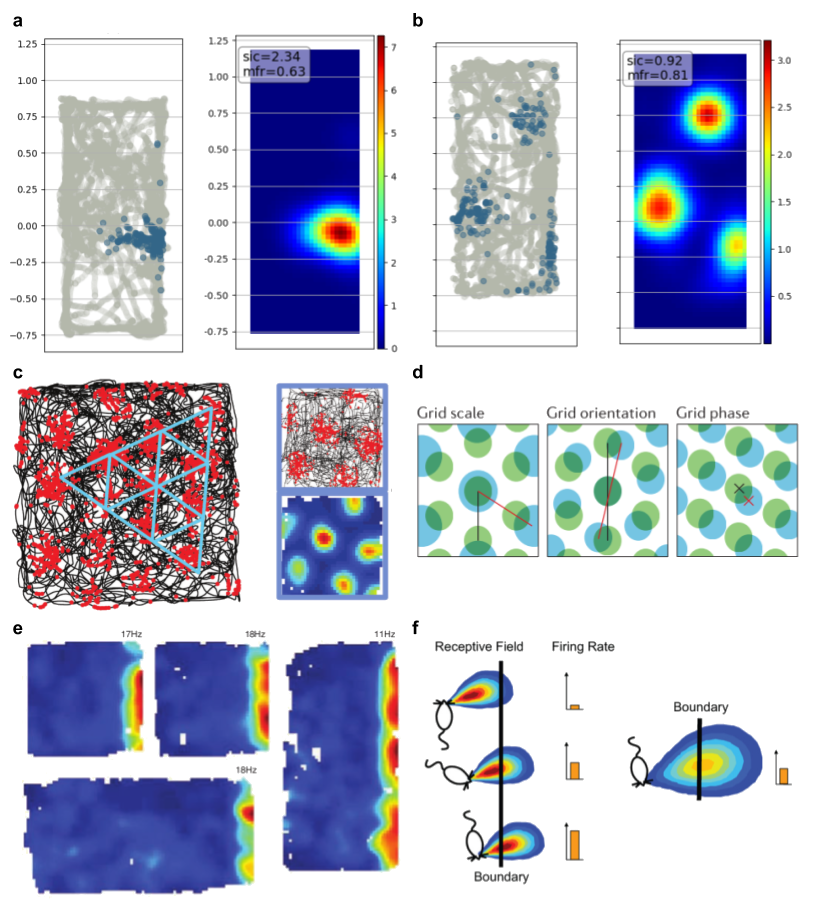
\includegraphics[width=150mm]{figures/F1_place_cells.png}}
\caption[Place and grid cells]{
Place, grid and border cells. \textbf{(a)} Firing rate map of an example hippocampal neuron that is active at a certain location in the rectangular environment - a “place” field. \textbf{(b)} another example neuron that has multiple place fields of different size (examples from the data used in the current study). \textbf{(c)} Firing rate map of an example mEC neuron that is active at certain locations of the environment, that form a hexagonal grid pattern (left). Place preference autocorrelograms reveal hexagonal structure (Adapted with permission from \cite{Moser2015}) \textbf{(d)} Examples of pairs of grid cells having different scale, orientation and phase (adapted with permission from \cite{Moser2014}). \textbf{(e)} Firing rate maps of an example neuron that is active near the right border of the environment, invariant of the environment type (adapted with permission from \cite{Solstad2008}) \textbf{(f)} schematic of the receptive field of an example neuron that is selective for a particular direction and distance to the environmental boundary (\cite{Lever2009}).
}
\label{fig:F1_place_cells}
\end{figure}


\subsection{Grid cells}

In addition to the discovery of the place cells, a few decades after, another important type of the place-selective cells were found in the brain’s entorhinal cortices. Particularly, in the layer II of the Medial Entorhinal Cortex (mEC) neurons, forming discrete regularly spaced firing fields were identified (\cite{Hafting2005}). Surprisingly, the firing fields of those neurons were organized in a grid of tessellating triangles evenly covering the corresponding space (Figure 1c). A simple autocorrelogram analysis revealed the rigid hexagonal structure (Figure 1c right). Key features of the newly discovered cells were, first - their different spacing between individual fields and phase shift relative to each other, with the increasing scale from dorsal to ventral mEC, and second - their anchoring to the boundaries, persistence between environments and independence on visual or olfactory landmarks. These facts suggest this type of cells is primarily based on self-motion and plays a main role in path integration, mixing idiothetic vestibular and proprioceptive signals.
Anatomically, mEC has a direct input to the Hippocampus. This led to the assumption that grid cells, sharing common peak and different spacing, might be a good basis to form place cells, taking grid cell inputs as a linear combination (\cite{OKeefe2005}). However, experimental evidence, based on studies on developing animals, shows that mechanisms are more sophisticated, as there is a delayed maturation of the grid fields relative to place cells. An alternative assumption, that place cells can be formed as a combination of the grid and other cell-type inputs - like border cells (see below), which are ready at the early stages of the development, looked to be more consistent. As suggested (\cite{Savelli2008}), specific place cells may arise as neurons integrating inputs from grid cells that provide proprioceptive-based distance information, and border cells that provide position relative to external boundaries. This putative idiothetic place cells will be named “boundary-driven” or “boundary-vector” cells later in the text.


\subsection{Head direction system}

One of the key components for successful navigation is maintenance of the proper allocentric orientation. Even before grid cells, neurons, which firing rates depend on the animal’s head orientation were found - originally in postsubiculum (\cite{Taube2007}), and later in other nearby areas (mEC, AdN etc.). Besides their primary feature of keeping the absolute directional preference, the “head-direction” cells were shown to maintain their relative directional preferences between each other; however, each cell by itself has no particular preference in absolute world coordinates - its directional preference can change between different environments. Importantly, in absence of light, head direction cells are able to integrate angular velocity of the head and maintain original directional preference, although for the cost of accumulation of directional error.

The presence of head direction cells is a necessary part to perform successful path integration, especially when light or external allocentric sensory cues are not present. The interaction of grid cells, providing distance estimation and a metric for space based on idiothetic inputs, and head direction cells supplying absolute orientation define the basis for position estimation based on path integration, which  is discussed more in one of the next sections of this chapter.


\subsection{Border and BVC cells}

While grid cells and head direction cells provide distance and orientation estimation, respectively, actual position should be estimated in relation to a certain point in space - usually relative to a physical boundary. Further research of the cell functions in the mEC lead to a discovery of the neurons representing geometric boundaries (\cite{Solstad2008}), and cells active at a particular distance to a certain boundary. These “border” and “boundary” cells are active when an animal is located near a certain physical boundary; their firing is independent of affine transformations (Figure 1e). A border cell, or more generally, a putative boundary vector cell (\cite{Barry2006}, \cite{Lever2009}), is another type of the neuronal encoding found in the mEC, that is involved in spatial representation. In a series of recordings these cells demonstrated preference to fire at a certain distance and direction to a particular object (Figure 1f) or, as a special case, to a certain boundary.

Border and boundary-vector cells (BVCs) may play an important role in updating positional signals of grid cells, as the latter tend to drift in open spaces. If the animal hits the boundary, any accumulated error in the grid cell positioning can be “reset” and appropriately corrected (\cite{Hardcastle2015}). Taken together, by defining the perimeter and stable physical objects relative to this perimeter inside, border and object-vector cells may represent an independent reference frame that can be used later by place cells to form correct space representations in the hippocampus.


\subsection{Landmark and object vector cells}

Besides environmental boundaries, stable visual landmarks can be used for building navigational strategies. In the visual sensory domain, cells, selective for certain spatial landmarks were discovered in the LEC (mEC) (\cite{Deshmukh2011}; \cite{Kinkhabwala2020}), and later in the CA1 and CA3 (\cite{Deshmukh2013}). These different selectivity types are ranging from an increase of neuron’s activity when passing a certain visual cue on the linear tracks (\cite{Kinkhabwala2020}), up to forming a stable firing field relative to a landmark at a certain distance and orientation. This discovery was further developed to a concept of general object vector cells found in the mEC, pointing to an idea that vector coding is a dominant form of position coding the entorhinal system (\cite{Hooydal2019}).


\subsection{Anatomy of the hippocampal-entorhinal system}

To establish meaningful conclusions about the mechanisms of the spatial navigation system, it’s important to explore the basic anatomical and functional connectivity of the underlying brain regions. Below we provide an essential extraction from the review of the anatomy of the hippocampal formation and the entorhinal cortex regions as the key areas involved in navigation, based on the rodent brain.

First we focus on the sagittal view of the rat’s right hemisphere, a horizontal brain slice in the middle of the hippocampal formation (Figure 2a). The hippocampal formation is presented by the key areas CA1, CA2 and CA3, as well as the DG and Subiculum. Darker areas show a density of pyramidal cell types (stratum pyramidale), where most of the place selective hippocampal neurons are found; lighter areas mostly contain dendrites and interneurons. The Parahippocampal region is represented by LEC, mEC, PrS and PaS areas. These regions contain the aforementioned grid cells and boundary-vector cells, as well as neurons selective to absolute orientations.

Pyramidal cells are excitatory cells that use Glutamate as a neurotransmitter. Different types of interneurons are all GABAergic (inhibitory), having their cell bodies distributed within all layers of the hippocampal formation (stratum radiatum, pyramidale, lacunosum-moleculare, oriens). Importantly, the activity of pyramidal cells are modulated by both external (e.g. mEC neurons) and internal (like CA3 principal cells and local inhibitory interneurons) inputs. One can distinguish principal cells and interneurons from electrophysiology. Principal cells have larger action potentials, have in average lower mean firing rate, and show noticeable bursty behavior.

The main cortical input to the hippocampus is the input from the entorhinal cortex that goes via the perforant pathway. Essentially this input conveys pre-processed information from higher-order sensory and association areas. In particular, most of the neurons of the layer 2 of the EC project to the DG and CA3, at the same time neurons in the layer 3 find their targets in the CA1 and Subiculum. CA1 and Subiculum provide feedback connections to the EC layer 5. There is a complex topography: all entorhinal layers are reciprocally connected (Figure 2b). In addition, there is also a mEC projection to the contralateral hippocampus with the same topography, although of a smaller density.

In essence, in the context of formation of place cells, the presented hippocampal-entorhinal connectivity allows for integration of the different mEC / LEC types of inputs with local CA3 inputs at the level of the CA1 pyramidal cells. This forms an anatomical basis for the assumption of the integration of grid, or boundary-vector cells, coming from the EC, with sensory driven cells - like visual landmark cells for the transient formation of the stable spatial representation in the form of place cells in the CA1 region.

\begin{figure}
\captionsetup{format=plain}
\makebox[\textwidth]{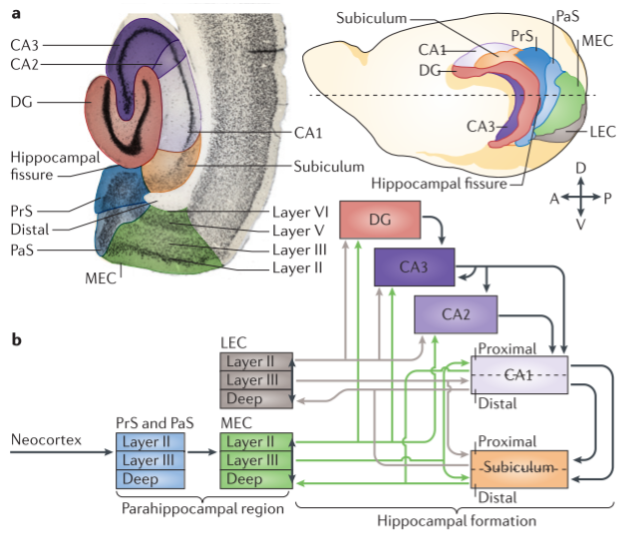
\includegraphics[width=150mm]{figures/F2_HPC_anatomy.png}}
\caption[Hippocampal-entorhinal Anatomy]{
(a) A slice of the right hemisphere of the rat brain (left). The focus is made on hippocampal and entorhinal regions. The same regions are shown located inside the rat brain (right). (b) Schematic of the connections within and between hippocampus and entorhinal cortex (adapted with permission from \cite{Moser2014})
}
\label{fig:F2_HPC_anatomy}
\end{figure}


\subsection{Sequence coding and theta phase precession in hippocampal cells}

As was established in the end of 1960x, hippocampal local field potential (LFP) activity provides oscillations of different modes and frequencies (\cite{Vanderwolf1969}). There are two main regimes - a prominent oscillation in a range between 7 to 12 Hz named Theta oscillation, and other irregular activity with broader spectrum of frequencies, including Gamma periods, Sharp-Wave Ripples (SWRs) and others. In rodents, theta oscillation highly correlates with animal actions and movements - running, jumping, grooming (\cite{OKeefe1993}). Here we focus on the theta regime and the corresponding animal behaviors, as they have an intrinsic connection with hippocampal cells.

Looking more detailed at these hippocampal place cells, an outstanding feature of the place cells behavior is their ability to lock their activity to a certain phase of the theta oscillation, when an animal runs through a place field (Figure 3a). While crossing a place field in one-dimensional or two-dimensional environment, place cell discharges in spiking bursts at progressively earlier phases of the theta rhythm, from spiking at peak of theta oscillation when entering a place field, having the highest firing rate (middle of the place field) on the trough to later spikes when exiting a place field on the ascending phase of theta oscillation (\cite{Jensen1996}, \cite{Skaggs1996}, \cite{Tsodyks1996}, \cite{Dragoi2006}).

This mechanism of spiking bursts within regular time windows is important for linking related path segments using the spike-timing dependent plasticity (\cite{Dan2004}). Importantly, the same mechanism might be useful for successful integration of the coherently incoming feature-extracted information of different modality, like the positional information relative to the spatial boundaries (boundary vector cells) and positional information relative to visual cues or landmarks (visual object vector cells), forming a unique spatial representation. More generally, the same mechanism, when used to integrate non-positional information like odors, sounds, or reward expectations, could be the basis of forming time-invariant memories, or episodes (\cite{Buzsaki2018}).


\begin{figure}
\captionsetup{format=plain}
\makebox[\textwidth]{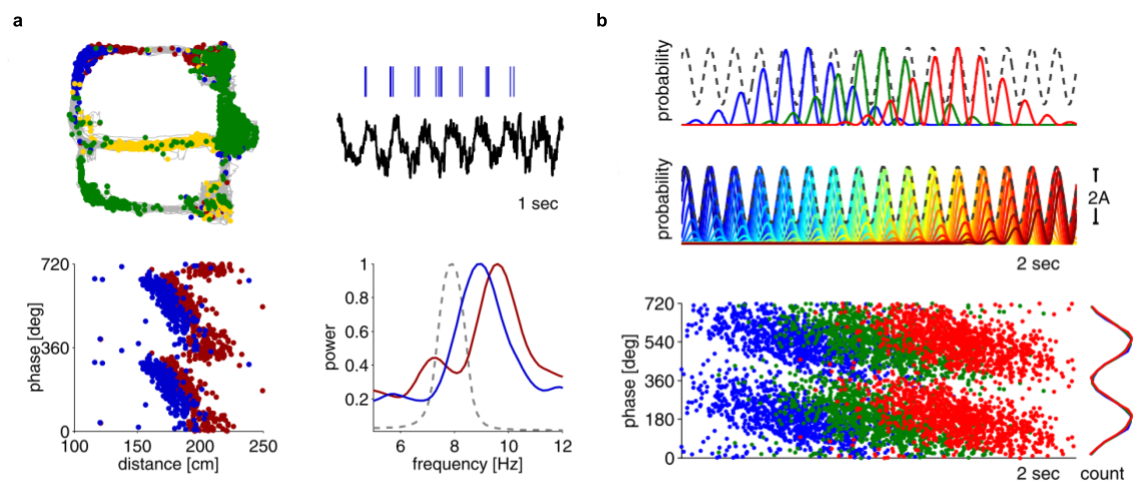
\includegraphics[width=150mm]{figures/F3_phase_precession.png}}
\caption[Theta phase precession]{
(a) A phenomena of the spiking precession of hippocampal neurons relative to the internal LFP theta oscillation. A neuron spiking is chunked by the oscillation and appears earlier in phase as a rat goes through a place field. (b) Sequences of memories and their interference (top), spiking phase relative to the theta oscillation (adapted from \cite{Geisler2010}; permission not required).
}
\label{fig:F3_phase_precession}
\end{figure}



\subsection{Formation of place fields}

Grid, border and head direction cells in the mEC together form one independent representation of space, stable between environments. The reciprocal representation is constructed by hippocampal place cells, that often fully remap between different environments, forming an unique representation of a particular space. These two spatial representations are complementary: one expresses the metric of a space independent of the specific landmarks or action-defined context, another is sensitive to the unique experiences in that space, location of objects or landmarks, building a number of context-dependent orthogonal representations.

The experimental evidence of the increased density of hippocampal place fields near corners and boundaries compared to the center of the environment (\cite{Wiener2737}) leads to a suggestion of a high level of a direct contribution of the border cells to the formation of place fields. Another fact supporting this hypothesis, is that border cells in the mEC are available in the early development - as do place cells when an animal explores an environment on the first day. This leads to an assumption that border cells might have a larger influence on place cells in youth, with the increasing role of grid and other types of mEC cells in adulthood.

Importantly, there is a bidirectional connectivity between hippocampus and entorhinal cortex (see - hippocampal anatomy), the latter receiving feedback from the hippocampus that may be essential for the formation or maintenance of entorhinal spatial maps. This is supported by the experimental evidence that the inactivation of the hippocampal inputs leads to the loss of hexagonal firing pattern of grid cells (\cite{Bonnevie2013}). These facts might be crucial for the explanation of the effects of place cell behavior presented in the results section.

To build experience-dependent representations, place cells need to interact with a variety of entorhinal cell assemblies, carrying distinct types of information. The efficiency and domination of different input types depends on intrinsic properties, like synaptic plasticity, but also on interaction with the environment - animal running speed, behavior, or environmental changes (\cite{Igarashi2014}). It is not yet clear if some of the input types dominate the other, and how place cells recruit synaptic inputs of a certain type to build stable spatial fields. In this work I try to address these questions and to demonstrate that in some particular conditions these inputs of allocentric and idiothetic nature are mixed, and try to further explore the dynamic balance between them.


\subsection{General questions}

The mechanisms that implement spatial navigation in the hippocampal-entorhinal system are not fully described and understood. Among open questions are the mystery behind the formation of the grid patterns, the phenomenon of theta phase precession, the role of gamma oscillations in memory consolidation, how and where the path integration is implemented and many others. Here in this study I focus on the phenomena of place cells in the CA1 region of the hippocampus, especially on the integration of the idiothetic, or precisely boundary-driven information and the visual, landmark driven information into a reliable space representation. The interaction between these allothetic and idiothetic inputs at the level of their postsynaptic influence, especially when they are in conflict, is not yet fully understood. Ultimately, these interactions may reveal, if described in detail, the more general mechanisms of episodic memory formation within the hippocampus which could be extended from navigation to a broad range of behavioral applications, including general action planning and abstract thinking.


%\section{The role of visual landmarks and physical boundaries in spatial navigation}
\section[The role of visual landmarks and physical boundaries in spatial navigation]{The role of visual landmarks and physical boundaries in spatial navigation%
              \sectionmark{The role of visual landmarks and physical boundaries}}
\sectionmark{The role of visual landmarks and physical boundaries}

\label{sec:role_of_landmarks}


\subsection{What is a place?}

A place in physical space can be uniquely defined by a set of reference points and landmarks, similar to it’s representative location on an allocentric map. Place is usually considered invariant of time and independent of the way how a subject gets there. This invariance connects the definition of place to the broader definition of semantic memory - invariant stable description of living things, facts or other knowledge (\cite{Buzsaki2013}). Repeated exploration of the environment allows subjects to revisit the same location multiple times, gradually building its representation from recurrent similar episodes - by linking together different (in time) episodes that share the same set of features, landmarks and relations between them.

High-level feature extraction is necessary to build a coherent representation of space, mainly because early sensory systems predominantly encode very simple stimulus modalities with very localized receptive fields. These would not be enough to build similar episodes sharing the same set of features, in case, for example, an animal reached the same location from opposite sides - and  experienced some different visual flow, experienced a set of new sounds, or made a different number of steps walking from the other boundary. Higher brain areas like hippocampus or cortical areas, involved in both memory and navigation, need to operate with higher order features like boundaries, objects of different shape, visual and olfactory landmarks, in order to be able to combine them as a set of similar combinations of sensory features (episodes) to an invariant representation of a particular location. As was shown in the first section, these operations of high-order feature selectivity might mainly reside in the mEC/LEC, being mostly implemented by boundary, object, and landmark vector cells. As anatomically hippocampus receives its major input from the entorhinal cortices, its role in navigation, shown by place cells, might be to orchestrate these incoming navigational information elements to either build and store a new place memory - a unique constellation of features, representing new location, or to update already existing place memory, if this set of features is similar to the already experienced number of stable objects, shapes and cues at a certain distance.

While external sensory information about distinctive and stable environmental features is necessary to build a stable allocentric map, the internal idiothetic information is required to both support this initial formation, as well as to maintain the constructed representation when the external information is partially or completely not available - for example, in total darkness. Our brains are able to maintain the allocentric position and navigate in space without external inputs, for the price of some error accumulation (\cite{Etienne1988}; \cite{Etienne2004a}). This is an indispensable function of the internal navigation system, essential for successful survival and evolution. The implementation of that feature requires an integration of the information coming from the internal idiothetic system into the circuits, encoding spatial maps. This aspect of establishing, recalling and maintaining the spatial map in absence of sensory inputs are discussed below in this chapter.


\subsection{Landmark and boundary vectors as reference frames to establish spatial map}

Overall, to build a spatial map one needs to define a set of related places (in the brain - place fields) having a certain position within a particular spatial reference frame. A reference frame can be defined as an independent coordinate system, having a definite distance and orientation to one or several reference points. Following this classical definition both environmental boundaries and a set of visually defined landmarks can serve as two independent reference frames, if they don’t change their relational stability between reference points within itself. When it is the case, the aforementioned landmark vector cells and boundary vector cells (\cite{Deshmukh2011}; \cite{Hooydal2019}) can be used to represent two reference frames of different modality in the brain.

While exploring the new environment, these inputs from the boundary vector cells and landmark vector cells (as well as other sensory modalities - olfactory, auditory etc.) are integrated to form coherent stable points, or recurrent episodes, which taken altogether, can be used to form a consistent allocentric representation of the surrounding environment. While moving from one place to another, animal revisits the places, formed of the similar set of environmental features, and reactivates the very similar sensory inputs which, with the help of some pattern completion mechanisms, updates and sharpens the CA1 ensemble representation of a particular physical location - place field in the hippocampal memory system. This movement from one place to another builds a trajectory - a set of connected physical places as an animal path, as well as the set of activated and connected places fields as a virtual path in the brain (\cite{Buzsaki2013}).


\subsection{Mechanisms of path integration to support navigation stability}


To maintain the navigational stability when allocentric cues are removed, the internal navigation system, including place cells, continues to track location using self-motion. Path integration is essentially a computation transforming a change in motion into a change in position. Having a current position estimate, one can derive a new allocentric position by tracking angular movements and distance travelled. Whether this system is based on continuous integration of angular or linear velocities, or on addition of a distance travelled vector to the current estimate - it is based on cues derived from the inputs from the self-motion systems (\cite{Etienne2004a}). These cues include vestibular, proprioceptive cues or motor efference copy (step counting). Additionally, a change in airflow (e.g. sensed by whiskers) or vibration from textures while moving can support speed calculation and resulting translation detection (\cite{Savelli2019}).

How can the path integration system be implemented in the brain circuits? While both distance and angular movement signals coming from grid and head direction cells tend to drift in open spaces without correction by particular cues or landmarks (\cite{Barry2007}), they are still the great candidates to support the path integration system. Boundary cells, or the tactile sensory inputs in the environmental corners, can episodically reset the grid and head direction inputs bringing the path integration system up to date with the environment position and orientation (\cite{Barry2007}; \cite{Cheung2012}). This leads to an assumption that path integration is mainly implemented in the cerebral cortex in a form of an attractor-network (\cite{Knierim2012}; \cite{McNaughton2006}), supported by the fact that the hippocampal upstream regions have all necessary components.

Another reported alternative is that the path integration computations are performed in lower regions, subcortically, reflecting the organization of the head direction system (\cite{Savelli2019}). As thalamic or other subcortical regions already receive vestibular and motor signals, they are able to compute and integrate angular and translational velocity signals, implementing basic path integration. The anatomical structure of the head direction system, for instance, with head direction cells found in anterior dorsal thalamic nucleus (\cite{Taube1995}) is another evidence to support this alternative.


\subsection{Impact on place cells}

Navigation at the level of hippocampal formation with its place cells are the main focus of this study. There is evidence showing that place cells follow visual cues (\cite{Muller1987}; \cite{Deshmukh2013}; \cite{Aronov2014}), suggesting that they receive incoming allocentric information. There is also a large evidence showing that place cells are able to maintain their place preference in case the sensory inputs are removed (\cite{Gothard2001}; \cite{Quirk1990}). In conflicting situations, as was shown in virtual reality (VR) studies (\cite{Gothard2001}; \cite{Haas2019}), cells are able to switch from one to another reference frame in their selective firing, suggesting integration of allothetic and idiothetic inputs. As described in the previous sections of this chapter, initial sensory processing and feature extraction, as well as path integration happens mainly outside the hippocampus. Taken together - how exactly these different pathways are integrated within the hippocampal neural circuits? This question is still not well understood. Below I review a few model studies exploring potential mechanisms of this integration (see modelling section).


\section{Research on interaction of allothetic and idiothetic inputs}
\label{sec:interaction_allo_idio}

One of the first seminal research studies of the effect of the allothetic environmental changes on place cells was done in 1987. Muller and Kubie (\cite{Muller1987}) showed that the rotation of a visual cue card, but not its width or shape, produces rotation of the place fields in a cylindrical arena. Removing the card led to a randomized angular representation of the arena. These recordings demonstrated direct dependence of the place field orientation on the visual information, implicating that cells in the hippocampus are modulated by allothetic visual inputs.

Getting more detailed, several years later, it was shown that objects located near the center of the arena could not control the orientation of the place fields in the environment, but do that with a help of a cue card on the wall (\cite{Cressant1997}). Same objects, placed near the walls enable control over the fields orientation, indicating that involvement of the head direction system, that potentially resets angular orientation relative to the unique objects, located close to the environmental borders.

The question of interaction of allocentric and idiothetic representations got more specificity in later studies by Bures and Zahalka (\cite{Bures1998}), where they experimentally trained animals to avoid foot shocks using either room landmarks or using idiothetically defined area on the floor. The ability of rats to avoid shock locations defined in both reference frames showed credible independence of the allocentric and idiothetic mechanisms, encoding two reference frames. However, a question of how these two systems are intermixed remained unclear.

Gothard and McNaughton proposed that place cells, mainly driven by internal “path integrator” - accumulated internally-driven translational information about a movement in space together with head direction cells - form a preconfigured network of a two-dimensional space. This network is updated by the visually-specific landmark information using associative learning (\cite{Mcnaughton1996}). They performed a series of experiments with rats on the linear track where two separate reference frames were used by a rat to track self position. By gradually moving these reference frames (a reward site and a starting box), they found both cells fired at fixed distances from the origin and cells fired at proximity to the destination. The same neuron was able to shift its spatial preference from being aligned to the origin to an alignment to the destination. They postulate that when mismatches between the visual and the idiothetic information occur, path integration and sensory cues competitively interact to affect place field preference (\cite{Gothard1996}). Their further recordings in light and dark conditions, showing that the box-referenced cells tend to keep their firing preference longer even without light, supported that idea. Ultimately, based on their moving-box-reward experimental data they suggest that interaction between internal dynamics and path integration and external sensory cues happens before both CA1 and CA3 areas, possibly in the entorhinal cortex or subiculum.

However the question of exact mechanism of position computation based on actual or path integrated information remained unclear. A new set of tools including virtual reality was introduced to continue the research of dynamics and circuitry implementing allocentric- and idiothetic- based navigation.


\begin{figure}
\captionsetup{format=plain}
\makebox[\textwidth]{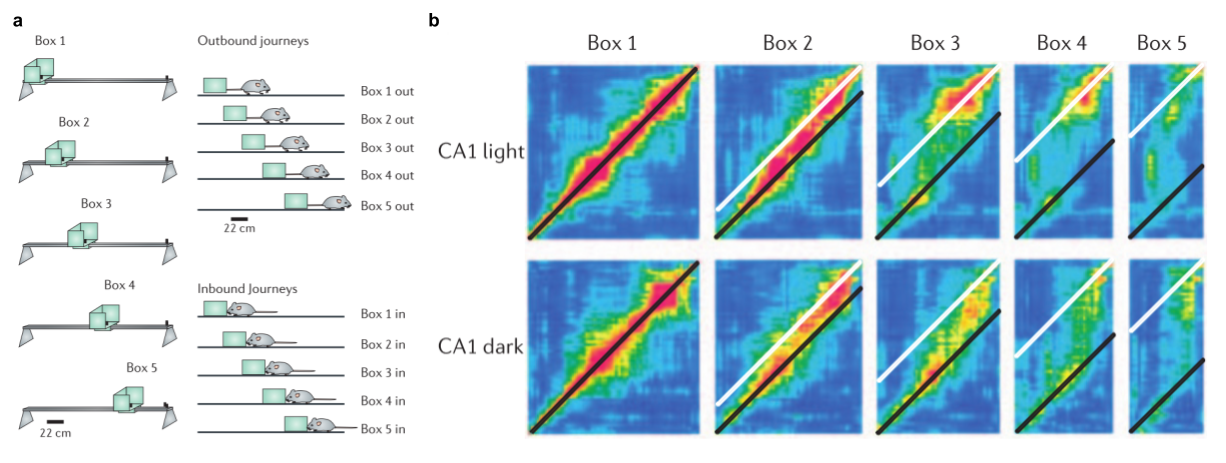
\includegraphics[width=150mm]{figures/F4_moving_box.png}}
\caption[Moving shelter as a reference frame]{
(a) A schematic of the experiment with a moving box. A starting box together with a reward location at the end of the track act as two independent reference frames. By gradually moving the box one can investigate the change of the spatial encoding relative to either of the frames. (b) The resulting place cell firing in light and dark establish gradual shift in encoding position (adapted with permission from \cite{McNaughton2006})
}
\label{fig:F4_moving_box}
\end{figure}


%\section{Optimal combination of environmental cues and path integration during navigation}
\section[Optimal combination of environmental cues and path integration during navigation]{Optimal combination of environmental cues and path integration during navigation%
              \sectionmark{Optimal combination of environmental cues}}
\sectionmark{Optimal combination of environmental cues}
\label{sec:optimal_comb_for_spat_nav}

How algorithmically do the allocentric and idiothetic inputs merge at the level of the hippocampal place cells? When the brain needs to integrate information of different sensory modalities it often uses “optimal” combination - a weighted sum of the inputs with weights proportional to their reliability. This has been established in many behavioral and theoretical studies for humans (\cite{Ernst2002}; \cite{Alais2004}; \cite{Knill2003}; \cite{Hillis2004}) for combinations of different sensory modalities (visual / auditory, visual / haptic, stereo / texture, environmental geometry / path integration etc.). The optimal coding theory is also applicable for spatial navigation. In a series of behavioral studies position estimation based on Bayesian decoding was established and predicted. In particular, optimal cue integration is demonstrated in ants (\cite{Wystrach2015}), rats  (\cite{Shettleworth2005}) or humans (\cite{Zhao2015}; \cite{Chen2017}; \cite{Sjolund2018}). However, while real-world navigation normally implies redundant integration of external, allocentric, cues and internal, idiothetic or path-integration based position estimations, is that combination always optimal?


\begin{figure}
\captionsetup{format=plain}
\makebox[\textwidth]{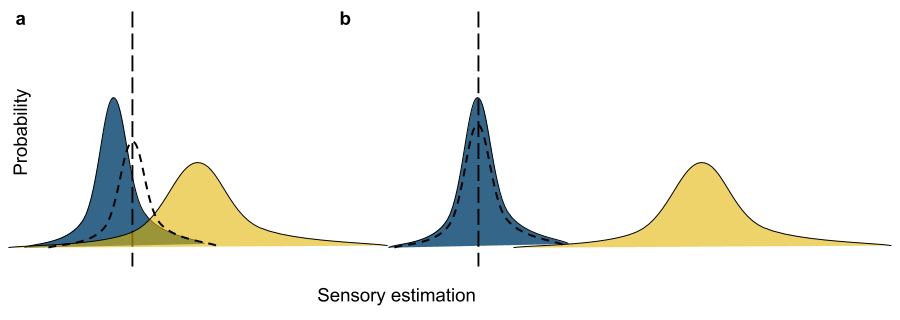
\includegraphics[width=150mm]{figures/F5_larger_smaller_conflicts.png}}
\caption[Sensory conflicts of different size]{
Sensory integration at larger and smaller conflicts. (a) In a situation of a small conflict between estimations it is beneficial to use optimal coding - a weighted combination of the estimation with weights proportional to their reliability (variance). Also named Bayesian decoding, or maximum likelihood estimation (MLE). (b) In a situation of a large conflict between estimations a strategy of abandonment of a less reliable information source will have higher chances to end with a better precision.
}
\label{fig:F5_larger_smaller_conflicts}
\end{figure}


Intuitively, when the conflict between two given estimations is small, weighted integration and resulting averaging makes sense. Especially if performed in an optimal, Bayesian way, it allows for a maximization of the precision of the resulting estimate, attributing a conflict to a sensory noise (Figure 5a). On the other hand, situations of a large conflict might be caused by misidentification of an object identity, incorrect memory retrieval or in general - failure in estimation based on a particular sensory source. In that case Bayesian integration might lead to large errors relative to both information sources, while full abandonment of one, ideally less reliable, source of estimate might be a logical choice (Figure 5b). This abandonment of one source, or cue, in favor of the other has been demonstrated in animal and human navigation studies. For instance, when humans were presented with a large > 115 degrees conflict between landmark and path integration cues they prefered path integration (\cite{ZHAO201596}). Rats in large spatial conflicts also prefer to rely on path integration in favor of a single landmark (\cite{Shettleworth2005}).

While the ability of a brain to implement optimal coding is well known, however it has not been thoroughly explored at the physiological level. Different potential schemes, including gain field theory, convolutional encoding, doubly distributional population coding were introduced (see review in \cite{Pouget2003}), however it is still not clear which scheme is used by the neurons or whether neurons actually encode continuous distributions at the population level. In this work, we address this question and make an attempt to show on the cellular level how these mechanisms of estimation integration at small conflicts and estimation abandonment at large conflicts could be implemented by a population of hippocampal neurons. We hypothesize that attractor dynamics in the hippocampal circuits might implement nearly-optimal coding for spatial and potentially non-spatial estimations, predicted earlier in other sensory systems (\cite{Jeffery2016}) and how the abandonment of less reliable estimation could be implemented at the level of a single neuron.


\section{Modelling multisensory integration at the level of place cells}
\label{sec:modelling}

“…Each place cell receives two different inputs, one conveying information about a large number of environmental stimuli or events, and the other from a navigational system which calculates where an animal is in an environment independently of the stimuli impinging on it at that moment. The input from the navigational system gates the environmental input, allowing only those stimuli occurring when the animal is in a particular place to excite a particular cell…” - an original sentence by O’Keefe led to a general proposal that the place cells might integrate idiothetic information coming from the different cell groups from the entorhinal cortex with some other sensory information.

Initially, a discovery of grid cells led to a model proposed by Solstad and Einevoll, which assumed formation of place cells via linear summation of weighted inputs from the grid cells (\cite{Solstad2006}). It was suggested that irregularly spaced place fields can appear as a result of summing inputs from entorhinal cells with different spacing and orientation, and relatively similar grid phases. However, this model was free from complex network interactions and required having place cells integrating grid cell inputs with overlapping vertices. This issue was fixed later by demonstrating that adding fast hebbian plasticity may result in the careful selection of appropriate inputs, without the need for specific network wiring (\cite{Savelli2010}).

The discovery of border cells and boundary vector cells led to another approach, assuming that environmental boundaries can serve as determinants of the hippocampal place fields. The boundary vector cell model (\cite{Barry2006}) describes place fields emerging from a combination of cells active at a certain direction and orientation relative to the environmental boundaries.

However, both of these approaches were focused on feed-forward type of information transfer, uni-directional communication between cortex and hippocampus. Recently, a novel approach connecting feed-forward information flow from the entorhinal layers to the hippocampus with feedback flow to the entorhinal areas, was proposed (\cite{Li2020}). It is a model that assumes continuous interaction between grid and place cells, with plasticity mechanisms enabling balance in control over place definition between vision and self-motion, allocentric and idiothetic inputs. In this model, self-motion is represented by multiple layers of grid cells that integrate angular and translational movement velocities (see grid cells). Visual input is modelled using a retina-like grid with Gabor filters, applied to the incoming stream of camera images. It is also assumed that it gets input from the head direction system such that the resulting visual information in particular location is independent from head orientation, similar to the non-grid cell in the LEC (see object-vector cells). Competitive organization of the network outputs establishes two different populations of place-selective cells - purely self-motion (or boundary) driven (motion place cells - MPCs), and purely visually driven (visual place cells - VPCs). These cells are assumed to be present in the CA3 regions of the hippocampus and together provide informative inputs to CA1 place cells. Having hebbian plasticity mechanisms and feedback connections back to the self-motion grid cells (MPCs), these latter CA1 cell are classified into 3 major groups - visually driven, self-motion or boundary driven and multisensory cells, that combine both of the allothetic and idiothetic inputs. These simulation results are very similar to the previously reported results (\cite{Haas2019}), as well as they highly correlate to the new electrophysiological data from the current study. Here I found very similar groups of neurons, having similar spatial firing properties (see Results). However, the disadvantage of the model is that it does not account for border-defined inputs which, as we also find in the neural data, might play an important role in correcting self-motion vectors and modulating the dynamics of the network as a whole.

Ultimately, considering models of the underlying neural dynamics, the current work is attempting to provide additional evidence for the modern loop-based approach to describe hippocampal-entorhinal networks implementing principles of spatial navigation. Based on the collected data, we hypothesize that hippocampal neurons implement a weighted combination of position estimation based on allocentric and idiothetic inputs in a nearly-optimal fashion. We show that the resulting position estimation influences self-motion based place representation, possibly via backprojections from the hippocampus to the entorhinal cortex. Overall this makes a step towards bringing evidence based on the neurophysiological data for the proposed model in situations, when place definitions are conflicting.


\section{Aim of the thesis}
\label{sec:aim_of_thesis}

For many years hippocampus has been identified as a brain structure, critical for spatial learning and navigation. The spatial domain extends beyond the traditional navigation in physical spaces - to many abstract spaces humans need to operate daily, not only to be partially efficient, but also to be successful in survival. Hippocampus, having specially tuned neurons - place fields - that rely on external sensory inputs and self-motion cues, mainly coming from the cortical areas, is able to implement high-level context-dependent representation of the environment. However it is still not known how exactly these different information flows interact to build a consistent and stable map of connected place fields.

Existing studies suggest that both proprioceptive and idiothetic types of information are continuously integrated to update the self-position (e.g. implementing “path integration”) while other stable sensory cues provide references to periodically update the allocentric position of self and correct it for the collected integration-related errors. It was shown that both allocentric and idiothetic types of information influence positional cell firing, however in most of the studies these inputs were firmly coupled. The use of virtual reality setups (\cite{Thurley2016}) made it possible to separate the influence of vision and proprioception for the price of not keeping natural conditions - the animal is usually head- or body-fixed (\cite{Holscher2005}; \cite{RavassardA.2013}; \cite{Jayakumar2018}), which introduces vestibular motor- and visual- conflicts, providing a bias for space encoding. Here we use the novel CAVE Virtual Reality system for freely-moving rodents (\cite{DelGrosso2018}) that allows to investigate the effect of visual- and positional- (vestibular) manipulation on the hippocampal space code while keeping natural behaving conditions.

Particularly, the current research is aimed at studying the impact of visual and vestibular (passive translation) manipulations on the hippocampal code using this novel freely-moving ratCAVE system. With the ability to manipulate the projected virtual environment and to unidirectionally move the physical arena depending on animal’s position, the following questions are addressed:

\begin{itemize}
  \item how would the stable visually-defined spatial reference frame impact the hippocampal place code when put in conflict with the moving space reference frame, defined by the physical boundaries
  \item would the passive physical move in space, locked to the physical boundaries and supported with vestibular inputs, differently impact the place code in contrast to the opposite situation when the move of the reference frame is just visual and not supported by the vestibular inputs - addressing the question of the role of vestibular information in coding the preference to one or another reference frame
	\item whether an instant mismatch between the visual and proprioceptive inputs (gain) would distort the hippocampal place map and at which threshold
	\item what types of the hippocampal place cells could be separated by their sensory and / or feedback inputs (visual, self-motion or boundary-driven or their combinations) and how strong is the path integration component
	\item whether a single instant conflict between information coming from the internal path integration system and the visual information can influence the current place code or lead to any remapping
\end{itemize}

In summary, we focus on the dynamic representation of space when the visual-cue-defined and physical-boundary-defined reference frames are in conflict. We confirm the dominance of one reference frame on the other on the level of place fields, when the information about one reference frame is absent (\cite{Gothard2001}). We show that the hippocampal cells form distinct categories by their input preference - surprisingly, not only that they are being driven either by visual / allocentric information or by the distance to the physical boundaries and path integration, but also by a specific combination of both. I found a large category of units integrating inputs from both allocentric and idiothetic pathways that are able to represent an average location between two reference frames, when they are in conflict. The use of virtual reality allowed me to demonstrate that these units become only path integrator driven when they lose their visual inputs. Based on the recorded information about these single cell theta phase-modulation, I propose a model how these units can integrate allocentric and idiothetic inputs to form this independent category of place representation.

Ultimately, the aim of the current work is to try to provide more support in linking the view over the hippocampus from the other side - to consider it not only as a spatial machine, but as a common generator of sequences of episodic memories (\cite{Buzsaki2013}), having place cells as examples of a particular recurrent episode - an integrated internal and external feature-processed sensory information at a particular moment of time, shaped by brain theta rhythms.


\chapter{Experimental Design and Procedures}
\label{ch:design}

\section{Using Virtual Reality to study navigation}
\label{sec:using_vr_navigation}


An efficient strategy that advances understanding of the complex spatial representation system is based on perturbation of one of its components. Experimental approaches using Virtual Reality systems (VR) allow to selectively perturb and manipulate visual cues. In recent years these systems have been widely used to study navigation (\cite{Holscher2005}; \cite{RavassardA.2013}; \cite{Aronov2014}; \cite{Thurley2016}).

The development of virtual reality (VR) systems for rodents (\cite{Holscher2005}) enabled scientists to manipulate environmentals properties, such as visual cues and landmarks in a fast and accurate way. It was shown that, despite the absence of the normal vestibular motion signals or tactile border inputs, animals are able to navigate in virtual coordinates, as well as their similar spatial neuronal metrics like place cells in the hippocampus are preserved. Chen and O’Keefe demonstrated that in VR, similar to the real environment, movement and visual information are combined nonlinearly in the place cell activity; the influence of one (visual) or another (proprioceptive) component varied significantly across cell population (\cite{Chen2013}). However, while being a good tool for sensory manipulation, body-fixed VR systems cannot fully model navigational processes in the brain - they do not only reduce theta frequency and speed dependence, but also reduce the number of active place cells and affect their directionality (\cite{RavassardA.2013}).

Although only simulating real environments and spatial navigation, VR systems opened a large door to the investigation of the neural behaviors when sensory inputs of different types are in an instant conflict. By introducing a gain-like difference between the speed of the visual projection and self-motion, one could establish a distinct population of neurons that either were locked to the salient visual cues or were strongly influenced by animal’s locomotion (\cite{Jayakumar2018}, \cite{Haas2019}). A set of experiments with continuous conflict between path integration and visual landmarks resulted in demonstrating stable and prolonged recalibration of the path integrator by the external information. This evidence supports the idea that visual cues do not only correct accumulated path integration errors, but can quickly reset the sense of position and update appropriate path integrator computation (\cite{Jayakumar2018}). The very recent work exploring hippocampal CA1 - CA3 regions shows highly context-dependent spatial coding in these regions (\cite{Zhao2020}), suggesting a high level of pre-processing of environmental features before they reach hippocampal formation.

Looking outside the hippocampus to the entorhinal cortex, gain experiments in VR revealed that border cells are mainly locked to the visual landmarks, while grid cells are modulated by both locomotion and optic flow. In the same set of experiments it was shown that the visual optic flow becomes more influential if it’s faster than expected (\cite{Campbell2018}). The recent mEC recordings show a new class of visual cue cells - neurons exhibiting firing fields near visual cues, consistently across different environments (\cite{Kinkhabwala2020}). This is another evidence that the entorhinal cortex contains both representation of landmarks and physical boundaries, - enough information to perform proper path integration.

However, while enabling outstanding opportunities for visual sensory input manipulations, conventional VR systems require animals to be body- or head-fixed. This poses a series of difficulties with animal training, imposing a different animal state (e.g. fear, aversion), as well as keeping some of the sensory information sources (e.g. vestibular, or olfactory) in a non-natural condition. These head- or body behavioral restrictions distort partially the vestibular and proprioceptive inputs and may lead to differential effects on place cell maps (\cite{Stackman2002}). Altogether this significantly impacts the navigation - both behavior and neural code.

To address these issues a freely-moving VR system ratCAVE was built (\cite{DelGrosso2018}). In contrast to conventional VR systems (\cite{Thurley2016}), ratCAVE allows for a natural animal movement and exploration in a rectangular arena, while retaining the possibility to manipulate distal and proximal (virtual) visual cues to influence animal navigation. It avoids vestibular motor and vestibular visual sensory conflict during locomotion, while constantly updating the surrounding virtual environment via the subject’s own freely-moving head movements, supporting natural perception and behavior. In addition, the ratCAVE setup (see Methods) enables to physically move the arena, partially distorting vestibular and proprioceptive inputs and changing the allocentric position of the animal.


\section{Experimental protocols}
\label{sec:protocols}

To study the role of different components of the allothetic and idiothetic systems on the hippocampal place code we introduce a conflict between different sensory inputs using Virtual Reality. We manipulate visual (virtual, projected) relative to the physical (defined by arena boundaries, tactile) reference frames as a key instrument to implement this mismatch while recording hippocampal CA1 neurons. By comparing the original condition, where both visual and boundary-defined reference frames are aligned, with the non-matching condition, where these frames are in conflict, one could study the dependency of the place cell activity on the navigation relative to one or another frame, as well as how intrinsic path integration would influence single unit activity.

\begin{figure}
\captionsetup{format=plain}
\makebox[\textwidth]{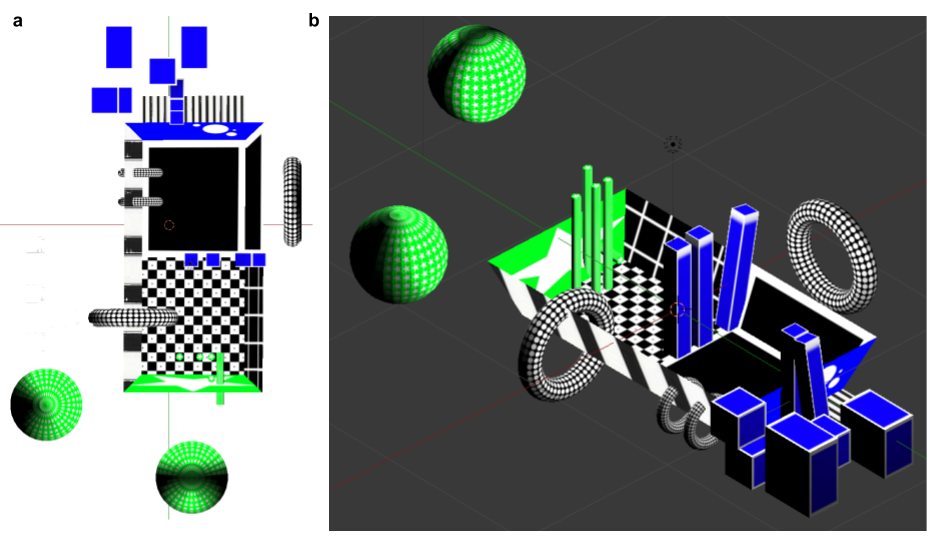
\includegraphics[width=150mm]{figures/F6_virtual_scene.png}}
\caption[Design of the Virtual environment]{
Model of the virtual environment for the ratCAVE Virtual Reality setup. (a) Top view of the Virtual environment for vSHIFT and vGAIN experiments (b) Same virtual environment viewed from the Blender modelling software to better see virtual objects and separation in three visually-distinct compartments.
}
\label{fig:F6_virtual_scene}
\end{figure}

The virtual environment consisted of the proximal and distal elements. Distal landmarks were unreachable, they consisted of two green spheres and several blue bricks located at some distance around the arena. The proximal landmarks are represented by landmarks on the arena walls - black and white stripes, black and white plaid, a grey star on a green background, together with distinct visual patterns on the floor - checkerboard pattern, black square pattern, stripes pattern, and virtual objects inside the arena - torus of several sizes, blue and green tall vertical bars. These objects and patterns supported the split of the virtual environment in three distinct “compartments”, which were chosen specifically to induce maximum visual influence on the animal visual perception system and engage more neurons in coding the visual reference frame (see Figure 6). For example, the “stripes” compartment in the vSHIFT -physical experiment is hidden in the original position of the arena, but is available to the animal in the shifted position. At the same time salient green bars on the other end are not reachable, which overall might induce visually-driven cells to more prominently react on the change.

For all shift and gain experiments animals were kept on the light food diet (about 90\% of ad libitum weight); animals were randomly foraging for food pellets inside the ratCAVE arena (see methods). Experimental time and movement protocols are described in detail in the following sections.


\section{Introducing mismatch between stable reference frames}
\label{sec:mismath_frames}

The aim of this experimental series is to identify the distribution of a subset of external sensory inputs (visual, tactile or boundary-defined) to the hippocampal place cells and the interaction of these inputs with the internal self-motion (proprioceptive, vestibular) signals, crucial for path integration. By probing whether the place fields would follow the 3D virtual visual reference frame or the physical boundary-defined arena frame one could split the influence of visual versus tactile (corner- or boundary- related) stimulus and determine how much they are influenced by path integration.

\begin{figure}
\captionsetup{format=plain}
\makebox[\textwidth]{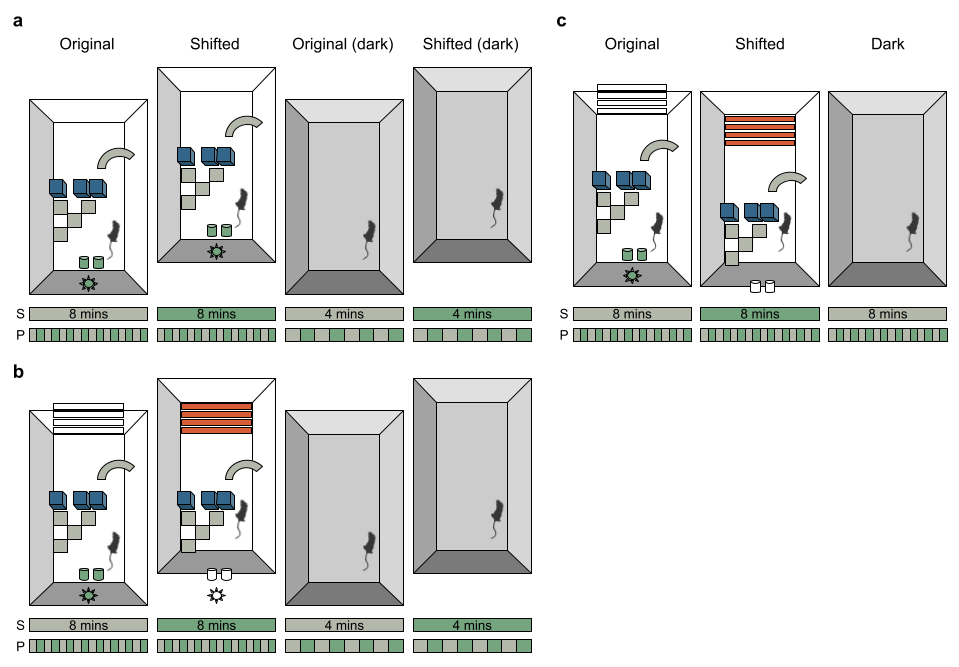
\includegraphics[width=150mm]{figures/F7_vSHIFT.png}}
\caption[vSHIFT experiment]{
Schematic of the concept of the vSHIFT experiment. For all plots: the green/gray bars on the bottom determine the protocol of the arena movement between original and shifted positions. S (single) - a single move, P (periodic) - translation every 30s. (a) vSHIFT - coherent. ratCAVE arena is translated together with the projected virtual objects and visual cues  back and forth along one axis, while the animal is randomly foraging inside. (b) vSHIFT-physical. The arena is periodically translated back and forth while the visual projection (virtual environment) is kept stable in room coordinates. (c) During vSHIFT-visual the arena is kept stable while the visual projection is translated further and back at the same protocol as in (b).
}
\label{fig:F7_vSHIFT}
\end{figure}


\subsection{vSHIFT-coherent - no conflict between reference frames}

To provide an evidence, that the external room cues (e.g. a projector and a mirror) do not play a role in formation of the spatial map, we designed an experiment where the both the arena and the visual scene were moving congruently together in the same time and spatial order as in the previous experiments. As these cues are subtle and hardly seen it is expected that they are ignored by the sensory inputs and do not influence spatial information in the hippocampus as well as the mechanisms of path integration. More precisely, it is expected that none of the units are able to fixate their spatial firing to the room reference frame, and all place fields would move together with the arena and the aligned visual scene. In addition to the experimental evidence of reference frame preference, the resulting distribution of the shift of the place fields could provide statistical metrics (e.g. standard deviation) for these particular conditions (arena length, animal size and behavior), useful for future analysis of other experimental conditions.

In this experiment both the arena and the visual projection were physically moved every 30 seconds in a longitudinal direction for 0.3 meters forth (shifted position, B) and back (original position, A), using the linear actuators located below the arena, like in the physical shift experiment. This action kept visual and border-defined reference frames aligned, while passively moving an animal in allocentric room coordinates (Figure 7a).


\subsection{vSHIFT-physical - conflict between vision and path integration}

In this experiment, a stable visual projection of the 3D virtual environment, containing proximal (virtual bars, torus and pillars) and distal (spheres) landmarks, was projected on the walls of the physical ratCAVE arena. This projection was stable in room coordinates for the whole experiment. To implement a shift, the arena was physically moved once or every 30 seconds in a longitudinal direction for 0.3 meters forth (shifted position, B) and back (original position, A), using the linear actuators located below the arena. The acceleration of the move was above the detection of the vestibular system, supporting the animal feeling of "being moved". As the projection was stable in room coordinates, it appeared to “shift” inside (relative to) the arena because of the arena move. This introduced a shift between the spatial reference frame, defined by the physical arena boundaries, relative to the visual virtually-defined VR reference frame (see Figure 7b). Neuronal activity was recorded during the whole session, and later only the times when the arena was stationary were analysed. For condition analysis, all periods when arena was in either original (A) or shifted (B) position were integrated to form two separate conditions A and B. For all animals, the session duration was ranging from 12 to 16 minutes, resulting in approx. 6 to 8 minutes of recording in condition A (12-16 arena moves) and 6 to 8 minutes in condition B (12-16 arena moves back).

For some sessions a 8 minutes period of an animal foraging in total darkness was recorded. These result in approx. 4 minutes of recording of the same neuronal units in position A and 4 mins in position B in darkness.

The shift of the arena to position (B) allowed an animal to enter a new virtual area, not available previously in original position (A). This area is marked by horizontal stripes (see Figure 7b, orange). Simultaneously, a virtual area at the end of the virtual scene (with green pillars), was no longer available in position (B) as the physical arena wall prevented an animal from going there. The salient visual landmarks (stripes, pillars) were specifically designed to be present in these areas to engage more place cells to change their activity in two shift conditions.

It is expected that this experiment allows to classify cells by their visual and/or self-motion or boundary-defined selectivity, thus suggesting their possible upstream input types. By studying the way the two different reference frames are represented by place fields may indicate the way the integration of these pathways is processed in the CA1 pyramidal layer.


\subsection{vSHIFT-visual - alternative way for a conflicting condition}

To probe whether the passive physical movement in space, supported by vestibular signals, is crucial for physical or visual reference frame encoding, it was asked if the shift of the visual scene alone could induce the shift in the encoding of the spatial map. Opposite to the previous physical shift experiment, here the visual projection, containing all distal and proximal virtual landmarks, was moved relative to the stable arena. In original position, the projected virtual scene matched the arena walls similar to the previous experiment, condition A. To introduce a shift, the visual projection was moved every 30 seconds in a longitudinal direction for 0.3 meters forth and back with the same timing, as it would take the physical arena to move. As the physical arena was stationary during the whole experiment, this move introduced a shift between the spatial reference frame, defined by the stationary physical arena boundaries, relative to the changing visual reference frame, with the exception that the animal was not physically moved in room coordinates and the vestibular input pathways were not stimulated (see Figure 7c).

This experimental condition is similar to the physical shift condition but without the translation of the animal and the arena in space. As the physical move engages vestibular inputs, this might influence the encoding of one or another reference frame in the hippocampus and might be interesting for a separate research.


\section{Introducing mismatch between vision and proprioception}
\label{sec:mismatch_gain}

The invention of different types of virtual reality setups for rodents (\cite{Thurley2016}) allowed to study the activity of the hippocampal cells when visual flow and self-motion are in continuous conflict. Tracking the position of the animal at high frequency enabled instant manipulation of the incoming visual flow inducing permanent gain mismatch between the actual translation (e.g. a real number of steps travelled) and the translation in the virtual space (e.g. the distance in virtual coordinates). Many studies claimed the ability of the hippocampal place cells to encode visual landmarks (\cite{Chen2013}; \cite{Aronov2014}; \cite{Jayakumar2018}) as well as the distance travelled (\cite{Haas2019}) in both gain and no gain conditions. However, as mentioned previously (see - using virtual reality to study navigation) in the head- or body-fixed VR systems some signals from the vestibular system (e.g. otoliths) are not present, while is has been shown that the vestibular system has a significant impact on the formation and stability of the place cells in general (\cite{Stackman2002}). Additionally, the ball-VR setups do not provide any real boundaries, making complex to bind position encoding based on self-motion to the environmental geometry. This series of VR experiments in freely-moving condition targeted to investigate effects on the hippocampal CA1 activity when there is either an instant or spontaneously induced mismatch between visual landmark-defined information and the self-motion, path integration defined information.


\subsection{vGAIN - shift via introducing a gain mismatch between visual flow and proprioception}

Another way of studying the preference for visual versus boundary-defined reference frames for spatial navigation is to introduce a gain mismatch between actual animal movement and the visual flow. Using the VR system, this can be implemented as essentially letting the animal move for a certain distance while moving the visual scene for the same distance multiplied by a coefficient.

To keep all the series of experiments compliant and comparable, we introduced the linear longitudinal gain of the visual flow of 1.2 and 1.5 between the virtual scene and the animal physical translation in a series of 3 stages: original no gain condition, gain condition (when an animal can access extended environment in VR coordinates) and again the no gain condition, when the virtual scene is shifted relative to the arena reference frame (see Figure 8a). Intuitively this experiment is similar to the physical or visual shift experiments (above), with the difference that the shift is performed with the transition via the gain period, when there is a mismatch between the animal longitudinal translation in physical and virtual coordinates.

Each period consisted of 6 minutes recording in every condition with 1 minute between periods, when the gain was linearly increased or decreased. This smooth increase of the gain was required to avoid instant change of the animal position in virtual coordinates and, as a consequence, potential remapping. For some sessions the dark period of 6 minutes was recorded. Recording cell activity in darkness can help in analysis and definition of cells, dependent on visual inputs and their firing behavior after the visual input is cut.

\begin{figure}
\captionsetup{format=plain}
\makebox[\textwidth]{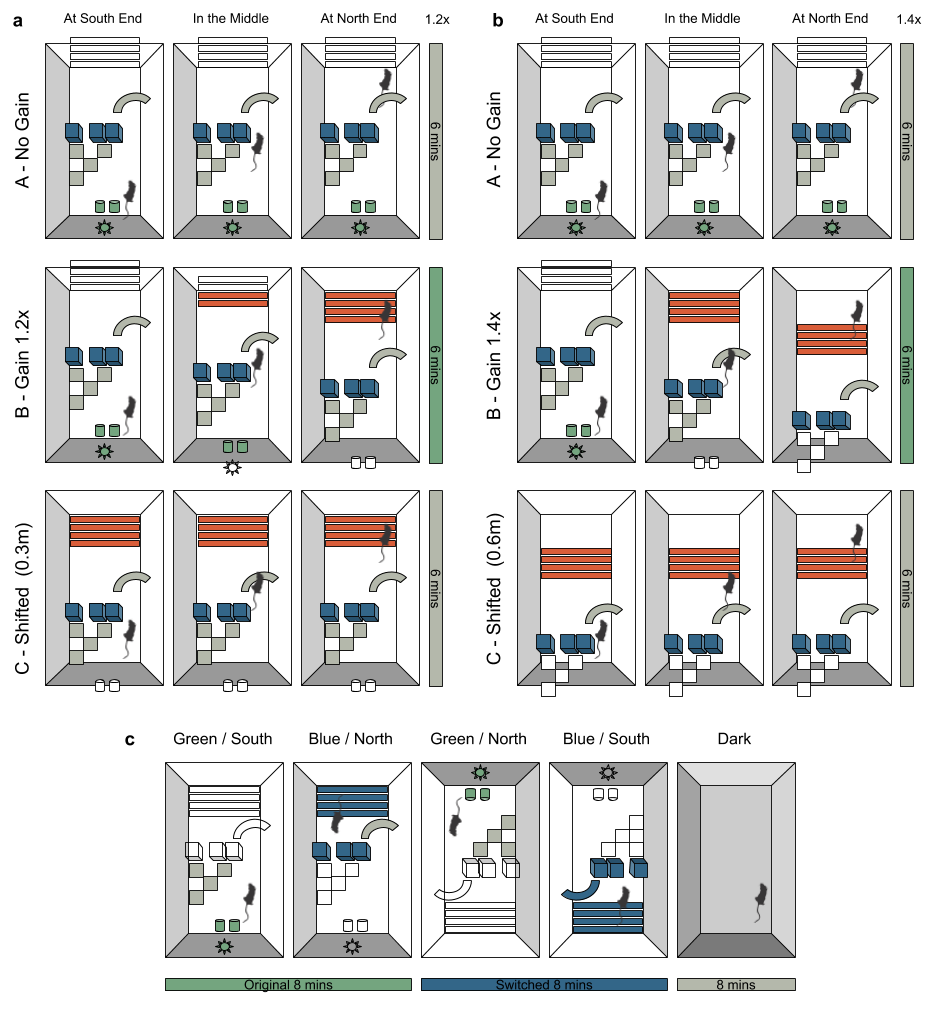
\includegraphics[width=150mm]{figures/F8_vGAIN.png}}
\caption[vGAIN experiment]{
(a) Schematic representation of the vGAIN experiment. Experimental session has 4 periods of original position condition when the animal learns the environment (top row), followed by a gain condition with the extended visual environment fit inside the same physical environment (middle row), and a shifted position condition, where there is no gain but the visual projection is shifted 0.3m relative to the original condition (bottom row). Some sessions followed by a navigation dark (4th period, not shown). Note the visuo-idiothetic spatial conflict between original (A) and gain (B) conditions depends on the position inside the arena (middle row, the conflict is largest at the north of the arena, while there is no conflict on the south of the arena). (b) The same protocol for the vGAIN 1.4x. The difference is the amount of instant (middle row) and resulting (bottom row) conflict ranging from 0 to 0.6m. (c) Schematic representation of the vTELEPORT experiment. Animals learn the environment where the green room is located on the south, and the blue room on the north. Note the projection for only one room where the animal currently is, is active at the same time (left two columns). After an exploration period, green and blue rooms are switched (green room goes north) bringing the conflict between visual cues and path integrator (middle columns). The main conditions are followed by a period of foraging in the dark.
}
\label{fig:F8_vGAIN}
\end{figure}


\subsection{Teleport experiment}

Place cells build spatial maps based on coherent sensory and self-motion-based representations. According to the accumulating evidence (\cite{Gothard1996}, \cite{Samsonovich1997}, \cite{Derdikman2009}) these maps are discrete for distinct environments, associated with unique experiences. Inconsistency between the actual sensory inputs and the recent position history, defined by self-motion and path integration, may introduce a specific type of remapping of the active place representation, referring to one or another discrete spatial map or having a mixture of components (\cite{Jezek2011}).

To study these effects on the level of hippocampal place cells, I designed a virtual teleport experiment. Using the freely-moving virtual reality setup, I designed an environment containing two visually distinct rooms of the same size, that fit the physical VR arena (rooms A and B). While an animal explores room A, the room B was not rendered, so only one room was visually available at a time. Crossing the midline of the arena allowed an animal to move between the rooms. Each room had a hidden circular spot, defined by the proximal visual cues, where an animal could trigger a reward if it stayed within the spot for more than 2 seconds. The rewards were continuously altered between rooms A and B to enforce an animal to navigate between rooms. After the initial learning of the environment for 8 minutes, rooms were switched at the earliest midline crossing, such that it appeared to the animal that it was entering the same room. The switch of the rooms was the central point to investigate whether the mismatch between the previous trajectory (path integration) and a newly imposed visual sensory cues would result in a map substitution or any other type of change in the corresponding place field representation (see Figure 8c).

Due to the time limitations only behavior, but not physiology was recorded with two animals. Behavior recordings demonstrate the ability of animals to learn the reward locations before the switch, as well as quick adaptation to the new orientation of the virtual environment after the room switch (see Figure 8c). This shows the significance of the visual-based virtual representation in original and switched versions and its very probable impact on the spatial map in the brain. However how this teleportation affects the place field maps remains to be investigated.


%\section{Comparison of hippocampal spatial activity between ball- and freely-moving VR systems}
\section[Comparison of ball- and freely-moving VR]{Comparison of hippocampal spatial activity between ball- and freely-moving VR systems%
              \sectionmark{Comparison of ball- and freely-moving VR}}
\sectionmark{Comparison of ball- and freely-moving VR}
\label{sec:comparison_ball_vr}

Previous research on the influence of sensory conditions on the hippocampal place code shows that inactivation of the vestibular system, which severely disrupts the head-direction system, was able to disrupt spatial maps in the hippocampus (\cite{Stackman2002}). While conventional ball-virtual reality systems impose behavioral restrictions such as head- or body fixation they distort parts of the vestibular and proprioceptive inputs, which may result in deformation effects on place cell maps. Understanding the levels of these distortions might be crucial to understand the contribution of self-motion cues to the expression of place fields. The presence of both types of virtual reality setups (ball-VR and ratCAVE VR, see methods and also \cite{Thurley2014}) on-site provided an opportunity to design experiments that compare neuronal activity involved in navigation between the setups, even in the same animal. By recording simple random foraging in the same virtual environment in body-fixed and freely-moving conditions, one could compare neuronal activation patterns, detect differences in place field firing and ultimately better understand the contribution of the vestibular inputs and physical boundaries on the hippocampal place map.

\begin{figure}
\captionsetup{format=plain}
\makebox[\textwidth]{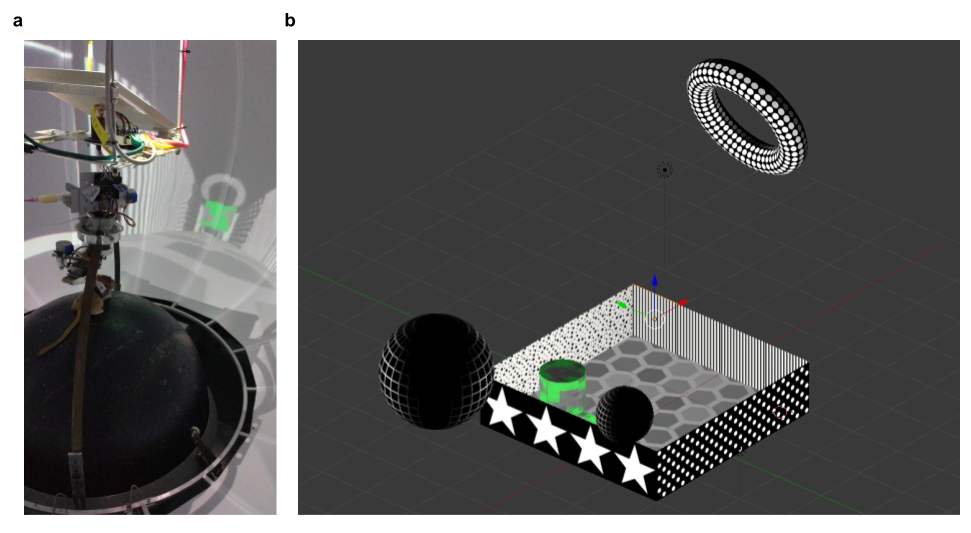
\includegraphics[width=150mm]{figures/F9_ball_VR.png}}
\caption[Ball virtual reality setup]{
Body-fixed virtual reality system. (a) A photo providing an overview of the setup with an animal inside. Animal is held in a harness fixed to the commutator that allows for a 360 degrees rotation. Running on a ball treadmill implements movement in the virtual environment, projected on the screen around the animal. (b) Schematic of the 2D virtual environment used in the beacon navigation task.
}
\label{fig:F9_ball_VR}
\end{figure}

To implement this experiment, I adopted the rendering engine and wrote experimental control software that enables the rendering of the same virtual environment in both VR setups (see methods). I designed a simple 2D environment and a beacon foraging task where gerbils need to navigate to a green beacon, which was changing its position every trial, to get a reward (20mg sucrose pellets in the ratCAVE setup, a 0.1ml dose of sweet milk in the ball setup).

While a freely-moving situation does not require any specific pre-conditioning, ball-virtual reality requires extensive handling and animal adaptation to being restricted by a harness. In gerbils, this restriction does not always lead to a successful animal adaptation and, empirically, depends on animal age, personal character and status in the cohort. As a result, many animals do not feel comfortable in the harness or even build aversion to both harness and setup. Practically this results in either animal freezing while being in the setup on the styrofoam ball, or a periodic running in a single direction, supposedly ignoring the visual projection, with an appearance aimed at escaping. Overall, such animal behavior even after extensive training and adaptation (4-5 weeks) does not always allow for navigation in a 360 virtual 2D environment. Actual training results show on average one out of four animals capable of adapting to the harness and setup, learning the 360 rotation, reward system and 2D navigation for a salient green beacon (not shown in this work). This imposes restrictions on the timing for the surgery: first - one has to train animals to select the right candidate, and second - it increases the risk of an overall wasted time, in case the surgery or recovery does not go well. Ultimately there was a decision to freeze this type of experiment until there is a better and more stable solution for animal training and harness adaptation.


\chapter{Results}
\label{ch:results}

\section{Example units and their conditional place firing}
\label{sec:example_units}

To get an intuition of place cell activity in different experimental conditions below I provide a series of examples of single cells. This is a qualitative, not quantitative visual analysis to get an overview of the types of place fields and their spatial preference in current experimental conditions. Quantitative analysis follows in subsequent sections.

In all 3 experimental conditions of a shift experiment (see introducing mismatch between stable reference frames) I recorded putative pyramidal cells from the hippocampal CA1 region from 9 animals; 521 of these cells were classified as spatially selective (see identification of single units). As some cells had multiple place fields, for the purpose of this study I’m going to focus on individual place fields instead of single cells as more relevant for the data analysis.

\subsection{Visually-driven place cells (VPCs)}

A total number of 176 place fields showed preference for the visual reference frame. Below we provide examples of a single unit firing, selective for particular features of the visual virtual scene, like:
\begin{itemize}
  \item a dark compartment of the scene (Figure 10a)
  \item an initially invisible part of the scene (Figure 10b)
  \item virtual pillars located in the middle of two compartments (Figure 10c)
  \item several virtual boundaries (Figure 10d)
\end{itemize}

\begin{figure}
\captionsetup{format=plain}
\makebox[\textwidth]{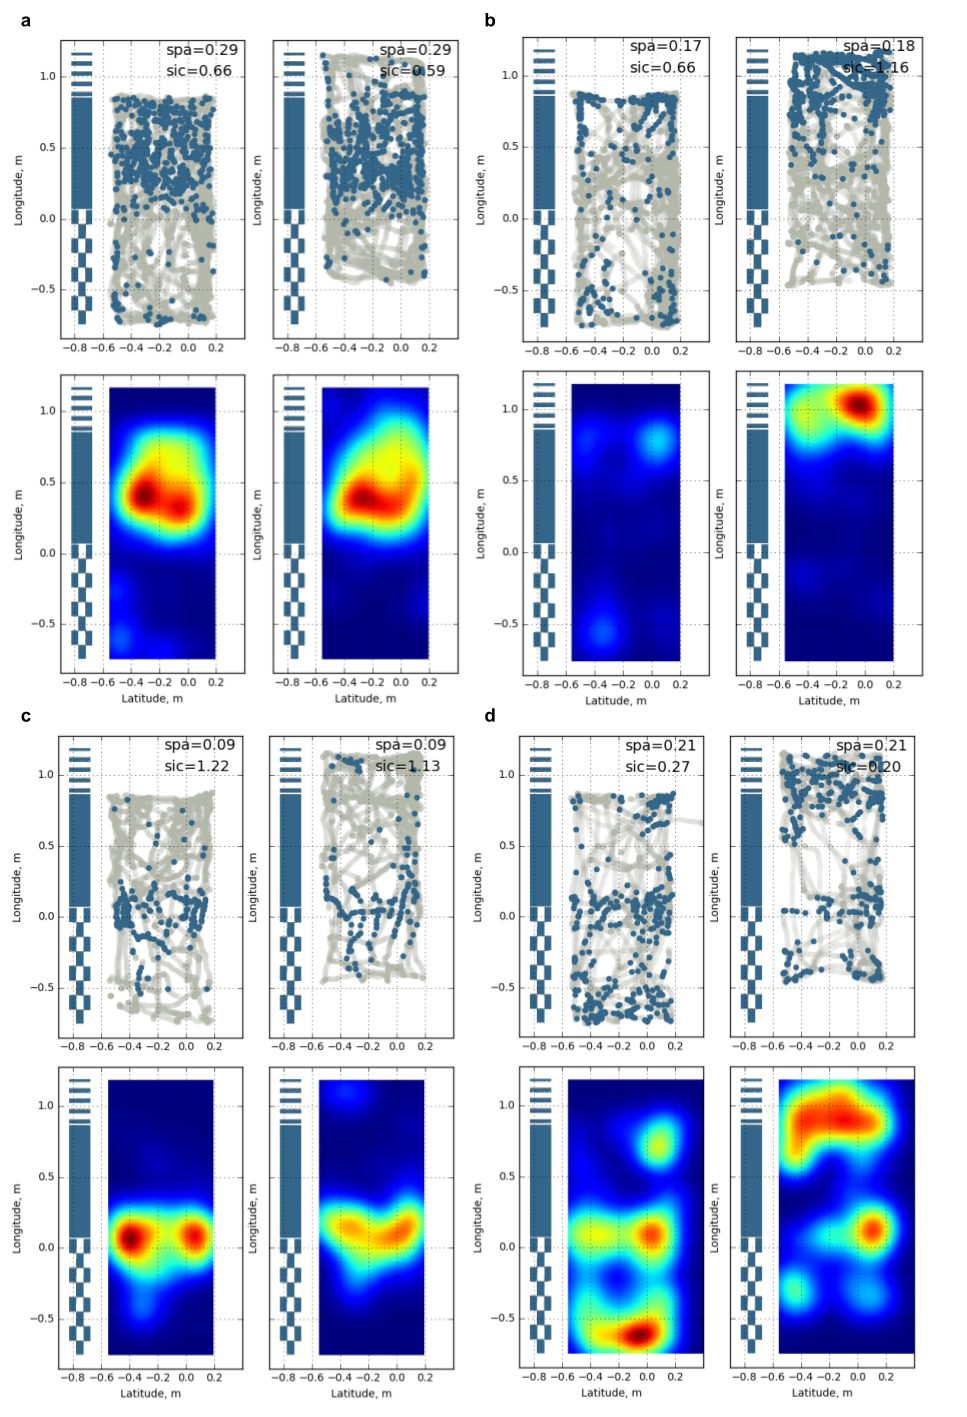
\includegraphics[width=100mm]{figures/F10_VPCs.png}}
\caption[Visually-driven place cells]{
Examples of visually-driven place cells. Each plot shows spiking (top) and firing rate maps (bottom) of a single neuron in the original and shifted arena positions. A ruler bar on the left shows schematic representation of the compartments of the (stable) virtual environment. \textbf{(a)} Cell selective for a dark compartment of the virtual environment. \textbf{(b)} Cell showing firing preference only for the initially invisible compartment, available only in the shifted position. \textbf{(c)} Cell selective for the virtual bars that make a virtual boundary inside the arena. \textbf{(d)} Cell showing preference to be active near physical and virtual borders.
}
\label{fig:F10_VPCs}
\end{figure}


\subsection{Self-motion or boundary-driven place cells (MPCs)}

A significant fraction (n=213, 29\%) of the recorded place fields showed preference for the arena reference frame. The Figure 11 demonstrates examples of the single units and their fields selective for physical arena boundaries:
\begin{itemize}
  \item for a particular corner of the arena
  \item for a particular arena boundary
\end{itemize}

\begin{figure}
\captionsetup{format=plain}
\makebox[\textwidth]{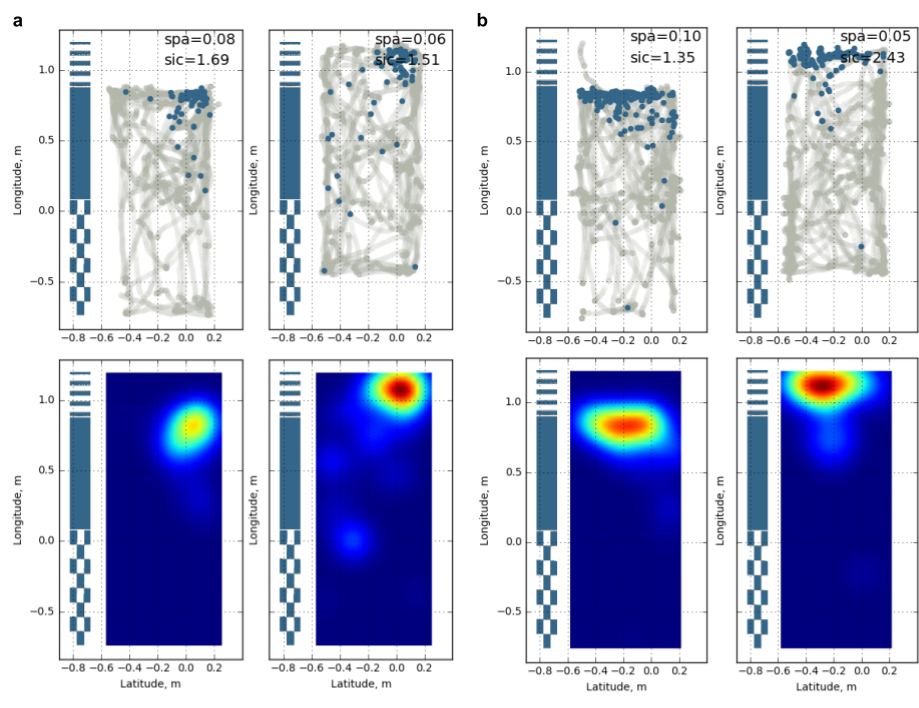
\includegraphics[width=100mm]{figures/F11_MPCs.png}}
\caption[Self-motion or boundary-driven place cells]{
Examples of boundary-driven place cells (2 cells). Each plot shows spiking (top) and firing rate maps (bottom) of a single neuron in the original and shifted arena positions. A ruler bar on the left shows schematic representation of the compartments of the (stable) virtual environment. (a) Cell active in a particular corner of the physical arena only. (b) Place cell showing preference for the upper arena boundary.
}
\label{fig:F11_MPCs}
\end{figure}


\subsection{Multi-field place cells}

On the Figure 12 I provide a couple of example cells that have multiple place fields.

\begin{figure}
\captionsetup{format=plain}
\makebox[\textwidth]{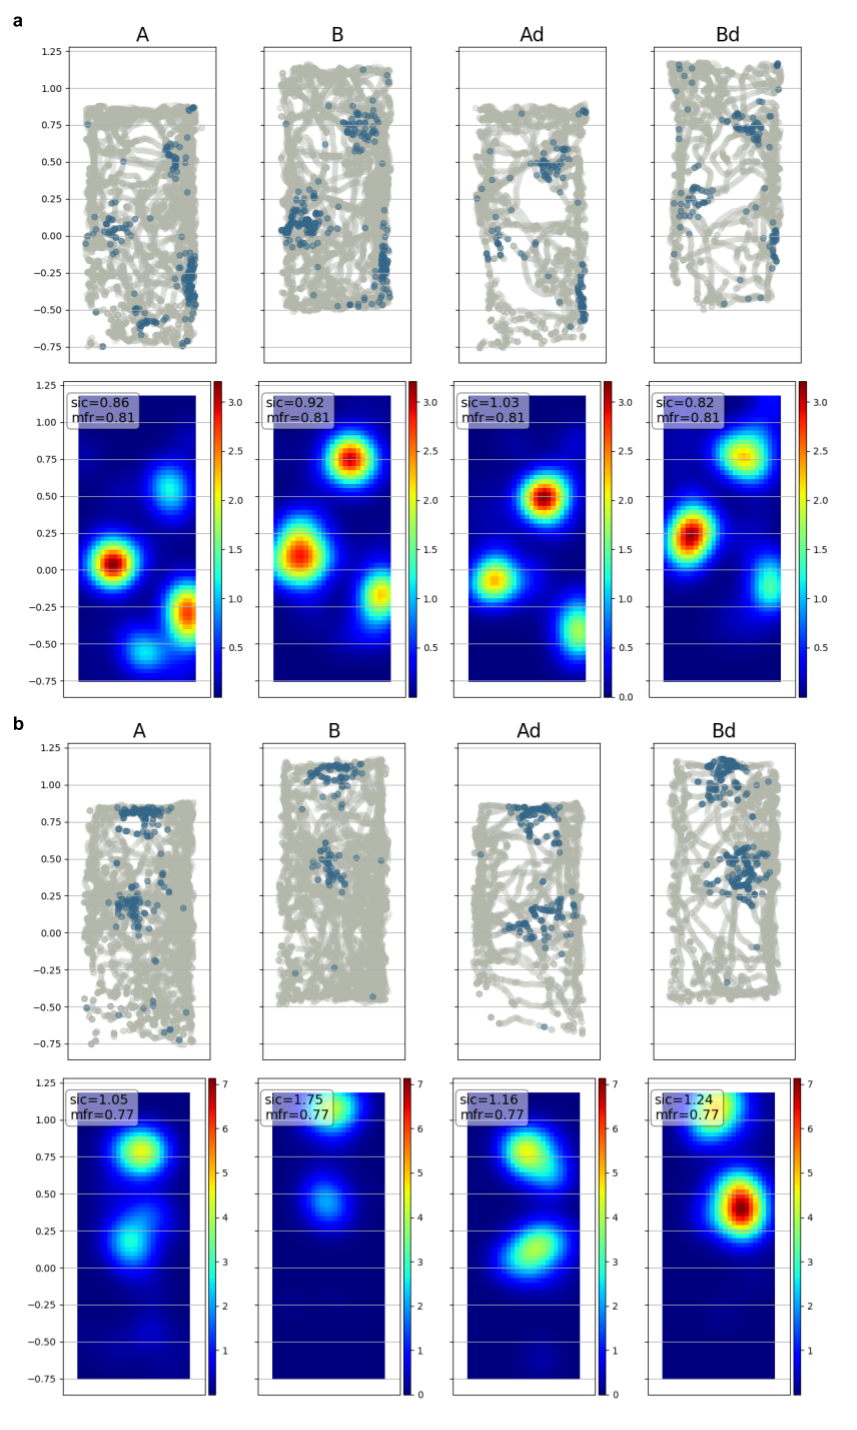
\includegraphics[width=150mm]{figures/F12_multi_field_cells.png}}
\caption[Multi-field place cells]{
Examples of multi-field place cells (2 cells). Each plot shows the schematic of the experiment (top), spiking (middle) and firing rate maps (bottom) of a single neuron in the original and shifted arena positions in light (A - B) and dark (Ad - Bd) respectively. (a) Example cell having three stable place fields. (b) Example cell having 2 fields locked to the arena reference frame.
}
\label{fig:F12_multi_field_cells}
\end{figure}


\subsection{Place cells integrating visual and self-motion components}

Recordings in conflicting sensory conditions revealed a non-bimodal distribution of place selectivity relative to the idiothetic and allocentric inputs. Many of the cells show weighted integration of both information pathways, encoding an average position. On Figure 13 is an example cell recorded in light and dark, original and shifted conditions. Note, the place field shift in light (left two columns) shows encoding of the average position defined by visual and boundary defined reference frames, while the shift gets bigger when the visual influence is lost (right column), illustrating integration of both information pathways.

\begin{figure}
\captionsetup{format=plain}
\makebox[\textwidth]{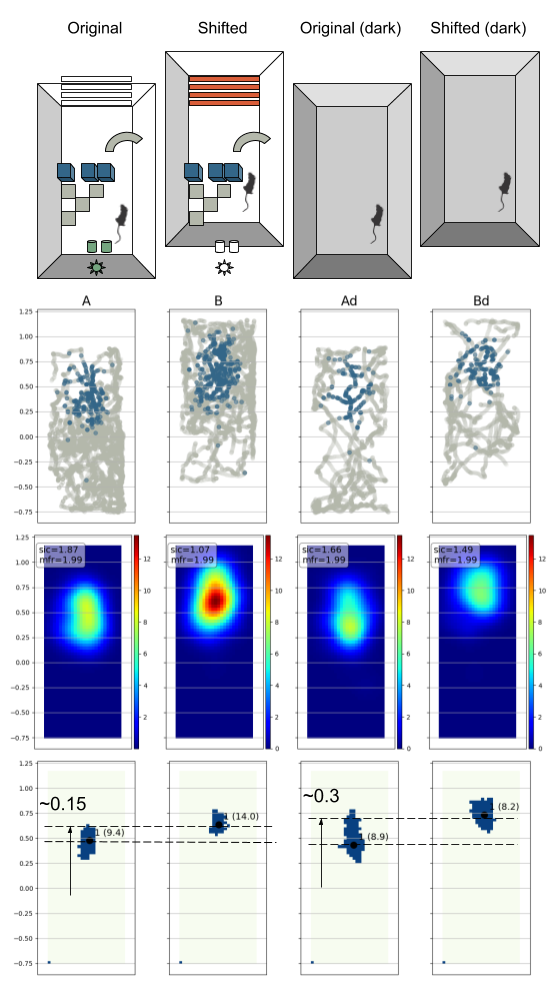
\includegraphics[width=100mm]{figures/F13_multisensory_cells.png}}
\caption[Multisensory Cells]{
Example of a multisensory place cell. Each plot shows the schematic of the experiment (top), cell spiking (second row), firing rate maps (third row) and place fields (bottom) of a single neuron in the original and shifted arena positions for light (left two columns) and dark (right two columns) positions. Dashed lines on bottom plots indicate the difference in place field shift between light and dark periods, indicating an influence of the visual information on spatial selectivity. Stability in dark shows integration of the self-motion inputs.
}
\label{fig:F13_multisensory_cells}
\end{figure}


\subsection{Multi-modal place cells}

A small portion (n=44, 6\%) of the recorded units is particularly interesting because these cells demonstrate two different types of place fields in both conditions, one encoding a particular visual landmark and another being selective for arena boundaries. Cells of this type can be identified by having one field stable between arena shifts, while the other field shifting together with the arena. These examples demonstrate an ability of a particular unit to simultaneously encode two reference frames of different type - visual and boundary-driven.

\begin{figure}
\captionsetup{format=plain}
\makebox[\textwidth]{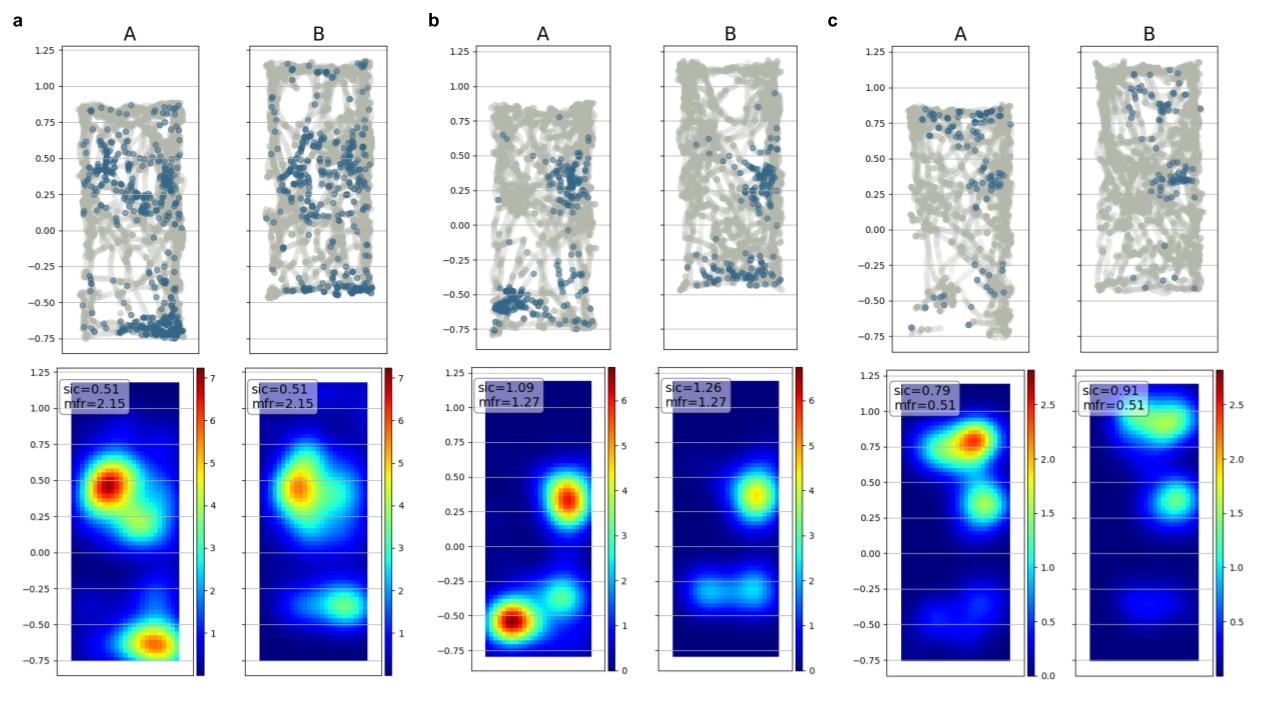
\includegraphics[width=150mm]{figures/F14_multi_modal_cells.png}}
\caption[Multimodal place cells]{
Examples of multisensory cells simultaneously encoding two reference frames. Each plot shows the schematic of the experiment (top), neuron spiking (middle) and firing rate maps of a single neuron in the original and shifted arena positions. (a) Place cell selective for the dark virtual compartment and the lower arena boundary. (b) Cell showing firing preference for the lower arena boundary and some location in the middle of the virtual environment. (c) Place cell selective for the upper arena boundary and also for some virtual location.
}
\label{fig:F14_multi_modal_cells}
\end{figure}


\subsection{Place cells expressing selectivity to specific virtual landmarks and visual features}

Several recorded units exposed specific place or domain selectivity. Figure 15 illustrates cells selective for both physical and virtual boundaries, or a cell selective for any place except a dark compartment of a virtual reference frame. These high-level encoding cells were mostly unique and cannot be statistically classified to a particular category.

\begin{figure}
\captionsetup{format=plain}
\makebox[\textwidth]{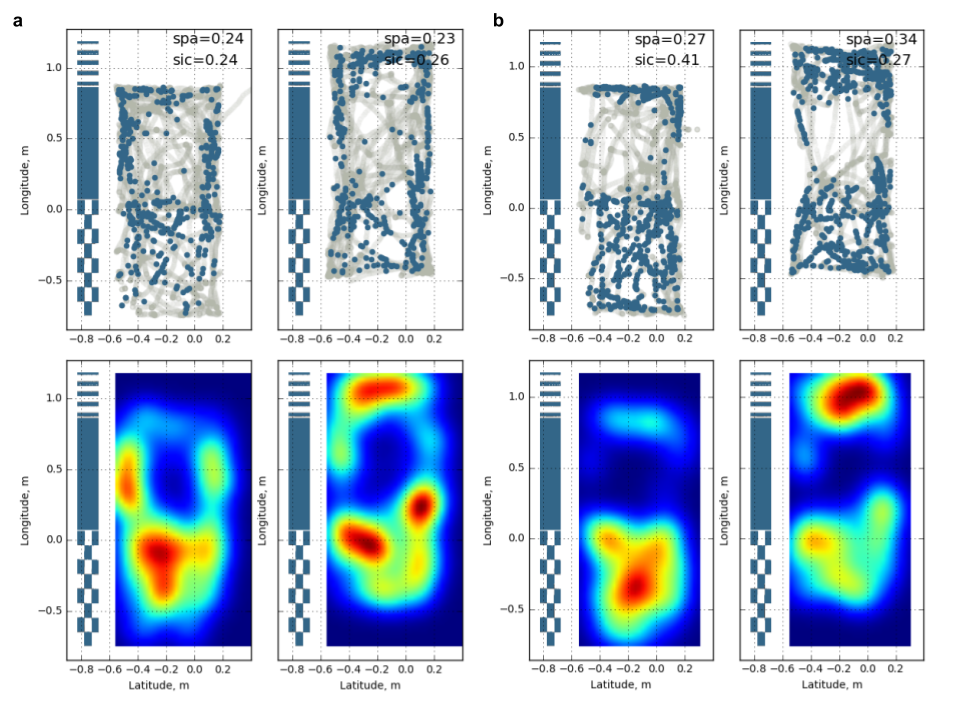
\includegraphics[width=100mm]{figures/F15_specific_cells.png}}
\caption[Specific place cells]{
Example units showing selectivity to specific virtual landmarks and visual features. Each plot shows firing rate maps of a single neuron in the original and shifted arena positions. (a) Cell representing a mixture of physical and virtual boundaries. Spiking activity near the middle of the arena corresponds to the virtual bars that make a virtual boundary. (b) Cell selective for any place in the virtual environment except a dark compartment.
}
\label{fig:F15_specific_cells}
\end{figure}


%\section{Place representation is based on enclosure geometry and proximal visual landmarks in VR arena}
\section[Geometry and visual landmarks forming place representation]{Place representation is based on enclosure geometry and proximal visual landmarks in VR arena%
              \sectionmark{Geometry and visual landmarks forming place representation}}
\sectionmark{Geometry and visual landmarks forming place representation}
\label{sec:env_geometry}

First, to establish a baseline of the behavior of the place cells and their navigational map in the non-conflicting allothetic and idiothetic conditions in the ratCAVE arena, I conducted the shift experiment with a coherently moving arena and the virtual scene (see vSHIFT - coherent). In this experiment, we expect CA1 cells to encode local visual cues and arena boundaries, ignoring global room coordinates. In fact, position in the global coordinates could only be derived from either the only visible cue in the experimental room - the mirror on the ceiling, or from the vestibular stimulation, coming from the moving arena, carrying a feeling of being passively moved. We assume that neither of the two options should be applicable as the mirror is located far from the animal and is almost not visible, as well as it’s been reported that animals hardly able to update their absolute position during passive shifts (\cite{Mittelstaedt1980}; \cite{Etienne1988}).

In total 119 spatially selective cells from 4 animals (see spatial firing maps and place field detection) were recorded and then analysed using the shift detection procedure (see place field shift detection). The shift detection procedure returns the position of each place field in the two different conditions - original and shifted. For this coherent translation case, if a particular place field has a shift between original and shifted conditions similar to the translation of the arena, this would indicate the field is moving “together” with the arena (and VR scene in this coherent case) and is locked to the non-conflicting arena/VR reference frame. Conversely, if the field has no shift between conditions that would display either its preference towards some globally positioned landmark, or its ability to compute  position estimation in global coordinates based on vestibular inputs.

The mean of the resulting place field distribution appeared at the shift of 0.28m in the global (room) reference frame given arena translation of 0.3m (see Figure 16). The absence of any distribution bias towards zero shows general preference for all place cells to encode arena / virtual scene reference frames, as expected. Although from these data one cannot make a full statement, one can assure that the total majority of hippocampal place cells in these conditions ignore any external stimuli (distal cues or vestibular inputs associated with arena displacement), encoding position inside the arena based on the arena boundaries and projected visual cues only. This allows to ignore any influence of these factors for future experiments. In the meanwhile, the statistics of these sessions (mean, SD) could be very practical for the subsequent analysis to quantitatively characterize the place field shift detection method for the recorded place field data.

\begin{figure}
\captionsetup{format=plain}
\makebox[\textwidth]{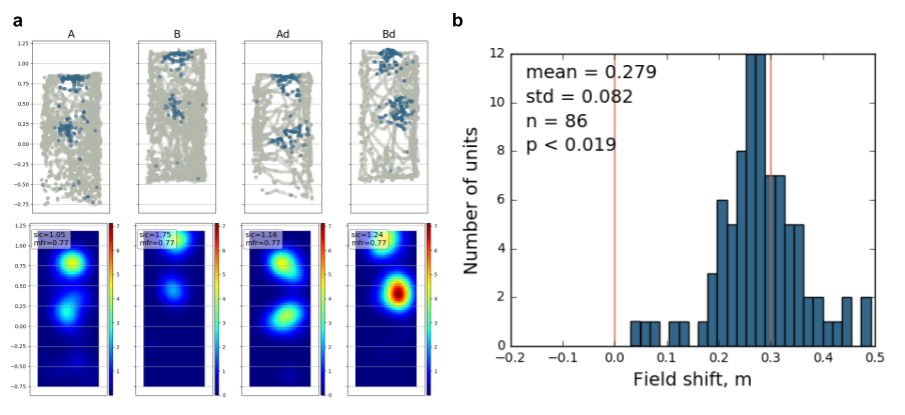
\includegraphics[width=150mm]{figures/F16_proximal_cues_geometry.png}}
\caption[Spatial orientation relative to proximal cues]{
Passive coherent movement of the whole environment (arena + visual projection) does not affect place fields firing. (a) example place cell with 2 place fields. (b) The distribution of the place fields shift between original (A) and shifted (B) conditions is centered near the actual shift of the whole environment, indicating spatial encoding based on the proximal visual cues and arena boundaries. A fraction of outliers might be due to mismatches in the shift detection procedure related with occasional low arena occupancy resulting in inaccurate place field centers.
}
\label{fig:F16_proximal_cues_geometry}
\end{figure}


%\section{Place field stability in darkness can be attributed to integration of self-motion inputs}
\section[Integration of self-motion inputs in darkness]{Place field stability in darkness can be attributed to integration of self-motion inputs%
              \sectionmark{Integration of self-motion inputs in darkness}}
\sectionmark{Integration of self-motion inputs in darkness}
\label{sec:integration_of_sm_imputs}

Assuming animals can only use local boundaries and projected virtual visual cues for self-localisation in the VR arena (see previous chapter), the only possibility to encode position in absence of visual cues (darkness) is to rely on integration of self-motion (path integration). If a particular place cell continues to fire in the same location in darkness indicates that it is driven either purely by self-motion, or by a combination of vision and self-motion when visual inputs are available (exceptions might be the place fields in the corners of the arena or in places where animal had left its feces, where the tactile or olfactory cues alone could define the absolute position within the arena). By quantifying the amount of place cells that keep their location preference between light and dark conditions one can build an assumption on how much of the self-motion component is integrated by the place cells in the non-conflicting (vision versus boundaries) sensory situation.

Using the field matching procedure (see place field shift detection), we split detected place fields (if a place field in original condition $F_a$ that has a pair in shifted condition $F_b$ it is one detected field F) into four categories. If a field $F_a$ has a corresponding field $F_a^{dark}$ in darkness, as well as its corresponding field $F_b$ has a pair $F_b^{dark}$ in darkness we classify this field as “stable”. If we cannot detect a corresponding pair field in dark condition for either $F_a$ or $F_b$, we classify this as “B-stable” or “A-stable” field, respectively. If neither of the fields $F_a$ or $F_b$ have a corresponding pair after the lights were turned off we classify this field F as “remapping”. The example on Figure 16 a) is a place cell with two “stable” fields.

\begin{figure}
\captionsetup{format=plain}
\makebox[\textwidth]{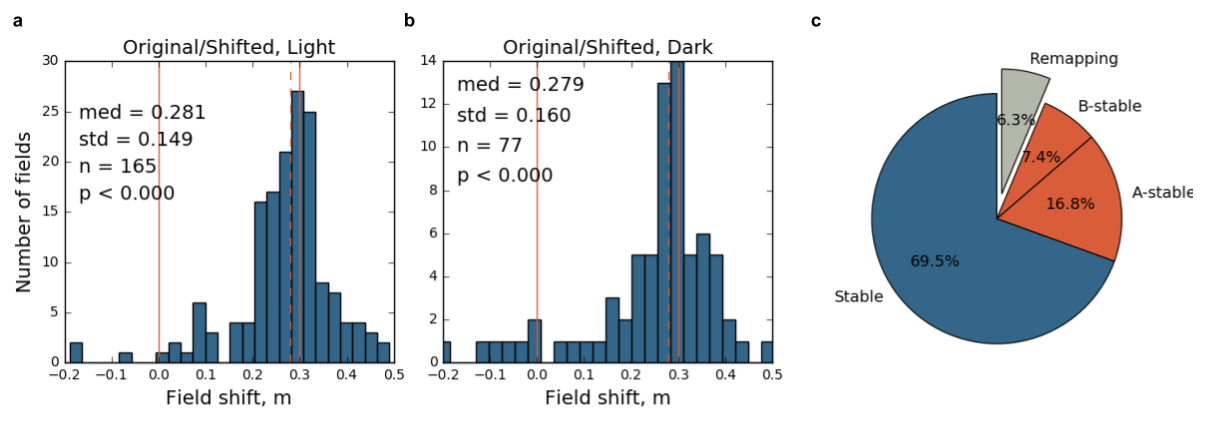
\includegraphics[width=150mm]{figures/F17_integration_of_sm_inputs.png}}
\caption[Widespread integration of self-motion inputs]{
The majority of place cells integrate self-motion inputs. Distribution of place field shifts in darkness (b) is similar to the light periods (a) in non-conflicting sensory conditions. (c) Fractions of place fields that can be tracked between light and dark periods. Only a small percentage of place fields (6.3\%) experience full remapping in darkness, indicating a high probability of integration of self-motion component for single cells, in line with previous reports (\cite{Allen6245}).
}
\label{fig:F17_integration_of_sm_inputs}
\end{figure}

A small percentage of place fields (6.3\%) experience full remapping in darkness, which could be attributed to the impaired path integration (\cite{Allen6245}). The relatively large (7.4 + 16.8 = 24.2\%) percentage of A- or B- only stable cells might be due to the decreased occupancy in the darkness condition (less running time, 4 versus 8 minutes in light) which led to the reduced quality in identification of place fields and false negatives in detection of place fields. Overall, the total domination of stable or partially-stable place fields between light and dark conditions (93.7\%) indicate that the majority of the place cells integrate position estimates based on self-motion inputs given non-conflicting sensory conditions (Figure 17c) and are not affected by the displacement of the arena with respect to the room coordinate system and are not controlled by the room-bound landmarks (mirror, projector, cameras etc).


\section{Simultaneous encoding of different reference frames}
\label{sec:integration_of_sm_imputs}

To investigate place cell behavior relative to the allocentric and idiothetic inputs we introduced a conflict between visually-defined and boundary-defined reference frames while an animal was randomly foraging inside the arena. A fraction (55\%) from the total recorded neurons (n = 521) in the vSHIFT-physical experiment demonstrate preference to either boundary-defined or visually-defined (examples in the section above) reference frame (see Figure 18a). This separation of place encoding in categories goes in line with already reported data (\cite{Mcnaughton1996}; \cite{Aronov2014}; \cite{Chen2013}; \cite{Haas2019}), however so far it’s been only shown for the cases of animal running on real track bound by reward-containing start/stop boxes or virtual linear tracks with VR-space contingent reward where it could be influenced by the reward bias. In contrast, here animals are freely-foraging  2D arena  for randomly scattered reward. Surprisingly, we found a significant number of cells (n=44, 6\%) having multiple place fields where each field was encoding a different reference frame (see Units encoding multiple reference frames). The ability of single hippocampal cells to simultaneously encode different categories of the same type of information (e.g. distal and proximal visual cues) was already presented (\cite{Knierim2002}), however this does not account for distinct types of information - visual and non-visual (self-motion or direct tactile and olfactory), presented in the current experiment. This suggests that hippocampal cells might pre-synaptically combine distinct types of sensory afferents and can be equally engaged in encoding different sensory modalities.

\begin{figure}
\captionsetup{format=plain}
\makebox[\textwidth]{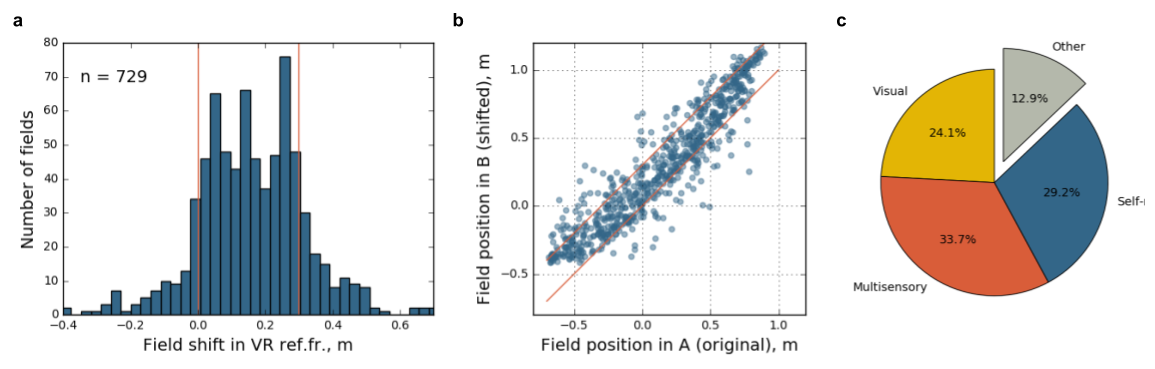
\includegraphics[width=150mm]{figures/F18_shift_distribution.png}}
\caption[Place field shift distribution in conflict]{
Place field shift enables classification of the CA1 cells into categories depending on their inputs. (a) Distribution of place field shifts between original (A) and shifted (B) conditions in the VR reference frame. Peak near zero denotes a group of place fields locked to the visual reference frame. Another peak near 0.3m defines fields encoding stable locations relative to the arena reference frame. A peak in the middle shows non-bimodal distribution of spatial selectivity in favor of a weighted integration of sensory inputs. (b) The same distribution as in (a) plotted against the position of the field in the arena in original (A) and shifted (B) conditions. Note the higher concentration of the 0.3 values near arena boundaries (bottom left and top right). (c) Overall classification of all place fields into 4 categories by their shift in conflicting sensory conditions.
}
\label{fig:F18_shift_distribution}
\end{figure}

Using the same shift detection procedure (see methods), the shifts in global (=VR) coordinates of a total of n=729 place fields from 6 animals were obtained from the recorded neural data (see Electrophysiology). The resulting place field shift distribution demonstrates place preference relative to the visual or boundary reference frames along the longitudinal axis, as well as the distribution of place fields along the arena (see Figure 18a). The distribution of place field shifts has 3 peaks around 0, 0.15 and 0.3 meters. On one hand, a non-uniformity of the resulting distribution suggests categorical structure of the underlying firing fields and corresponding neuronal mechanisms. On the other hand, a presence of the large group of place fields (n=246, 33\%) encoding average between reference frames suggests possible continuous weighted integration of visual and self-motion sensory components (see discussion about weighted integration).
A light domination of the boundary-driven over the visual place representation preference (29\% versus 24\%, cells attributed to each group by having a place field shift of 0.3m (+- ~1 SD = 0.075m) or 0.0m (+- ~1 SD = 0.075m)) can be explained by the initial larger influence of the boundaries while initially exploring the environment (\cite{Keinath2018}). Another reason can be that the recordings were made from mainly distal, not proximal CA1, which is known to get more input from the mEC representing idiothetic inputs, rather than LEC, better known to provide allothetic sensory information (\cite{Knierim2014}).

According to our analysis, a place field shift near 0 m defines a group of place fields, stable relative to the landmarks in the virtual scene during physical arena displacement (24\% cells). This allocentric stability in virtual space could be explained by a profound drive of the hippocampal cells by visual inputs. This type of neurons having fields mainly driven by vision was already established (\cite{Muller1987}; \cite{Chen2013}, \cite{Haas2019}). Another possibility would be that this group of cells receives both visual and self-motion inputs, but the self-motion component is weak and is fully reset by visual landmarks every time the animal appears to be navigating near virtual cues away from the borders. The appropriate evidence for that hypothesis still needs to be found and it is being discussed later in the following chapters.

A place field shift near 0.3 m includes a number of place fields that move together with the boundary-defined reference frame. A presence of this type of location encoding can be explained if either cells would be driven by self-motion inputs away from arena boundaries (the idiothetic path integrator, trajectory integration relative to the arena walls) or by a direct tactile contact with borders (e.g. inputs from border cells).

Similar results of separating groups of place fields into visually- and boundary-driven categories was reported in several studies (\cite{Chen2013}, \cite{Haas2019}). However a third category of place fields, representing an average location between visual-landmark- and boundary-defined reference frames, was not yet explicitly found and investigated.

To test if this category of place fields appeared by chance the random simulation procedure as there would be only two visual- and boundary- cell categories was performed. Assuming there is no average position encoding, the overall distribution of the field shifts could be represented by a sum of two gaussian distributions (visual and boundary categories) with means of 0, 0.28 and SD of 0.82 (values taken from the original vSHIFT - coherent experiment) having sample proportions as the ratio of the actual peaks around these means (1:1.2). The random simulation of such a sum of distributions reveals a 0.00001 chance of 0.33\% of all samples (246 out of 634 fields) falling between 0.075 and 0.225 (middle shift range). This is a strong evidence that this category is not a result of a chance coming from experimental recordings.


%\section{Balance in availability of a certain sensory modality determines position encoding at the population level}
\section[Sensory availability determines position encoding at the population level]{Balance in availability of a certain sensory modality determines position encoding at the population level%
              \sectionmark{Sensory availability determines position encoding at the population level}}
\label{sec:balance_sm_vs_vision}

According to the previous reports (\cite{Mcnaughton1996}; \cite{Gothard2001}) and subsequent reviews (\cite{Maaswinkel1999}) it is hypothesised that in conditions, where different spatial reference frames are in conflict with each other the place code shows a hierarchy of preferences (\cite{Maaswinkel1999}). In particular, in absence of immediate boundaries or away from the boundaries visual cues can take over. In the vSHIFT-physical experiment, the distribution of the place field shifts reveals the higher concentration of the visually-driven fields in the center of the arena (e.g. away from the northern and southern arena boundaries), while having a higher concentration of boundary- or self-motion driven fields near the borders (see Figure 19a, b). This could be explained by a competition of boundary-driven self-motion and visual inputs. Close to the environmental boundaries the direct tactile contact engages additional sensory modalities, while the quality of visual projection decreases. Away from the boundaries all the visual cues are instantly available while the precision of the self-motion based inputs decays with time and distance travelled since the last boundary, although not that fast to be very distorted in current experimental conditions (\cite{Hardcastle2015}). This allows to hypothesize, that if a place cell encodes a combination of the self-motion and visual components, the contribution of the visual one would be larger in the center of the arena, setting a higher weight for that type of an input. Opposite, near the boundaries the contribution of tactile / self-motion component would overtake the vision and a place field input weights would be more balanced towards self-motion. More of the interpretation of these findings in the discussion.

\begin{figure}
\captionsetup{format=plain}
\makebox[\textwidth]{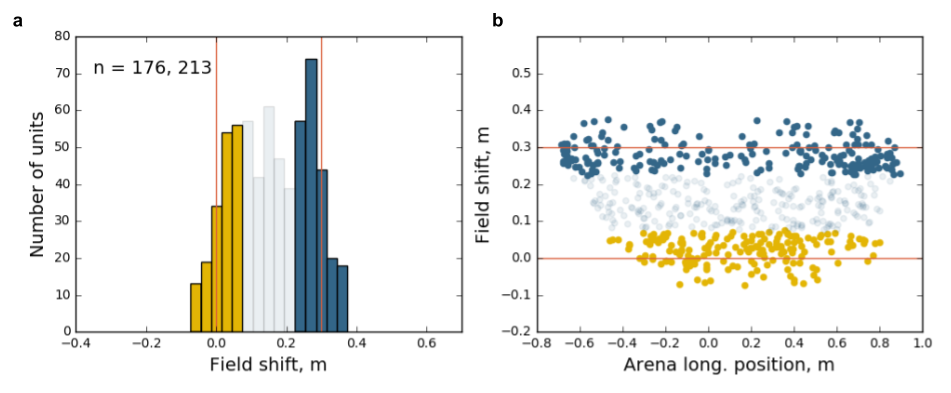
\includegraphics[width=150mm]{figures/F19_balance_field_concentration.png}}
\caption[Balance between vision and self-motion]{
Balance in concentration of fields of different types (vision versus self-motion) in the center versus near the boundaries of the arena demonstrates a tendency to prefer more available sensory input for spatial encoding, potentially implementing optimal coding at the population level. (a) Distribution of place field shifts between original (A) and shifted (B) conditions with visual (yellow) and self-motion (blue) groups highlighted. (b) Place field shift plotted against position in the arena. Visual and self-motion groups highlighted as in (a).
}
\label{fig:F19_balance_field_concentration}
\end{figure}


%\section{Removal of allocentric information reveals a group of multisensory CA1 cells to be driven by a combination of vision and self-motion}
\section[Multisensory cells driven by a combination of vision and self-motion]{Removal of allocentric information reveals a group of multisensory CA1 cells to be driven by a combination of vision and self-motion%
              \sectionmark{Multisensory cells driven by a combination of vision and self-motion}}
\sectionmark{Multisensory cells driven by a combination of vision and self-motion}
\label{sec:multisensory_integration}

To further investigate the interaction of the hippocampal place cell afferents, we recorded several sessions of the original vSHIFT-physical experiment having a darkness period after the main session time. This allowed to analyse the change in spatial selectivity for place fields, especially the fields driven by a combination of visual- and self-motion inputs, when the visual input together with the whole virtual reference frame are absent. Essentially by looking at the change in cell activity - change in firing rate, field size, field shift or complete re-mapping - we can hypothesize how the reduction of sensory input, in particular, visual information influences place cell binding to a specific reference frame.

For the light periods, place field shift distribution for sessions with darkness is equivalent to the regular shift experiment sessions (see Figure 20a). However, taking the darkness periods alone, all identified place field shifts are centered around 0.28m with no substantial amount of fields near 0.0m, showing their preference to encode the boundary-defined reference frame (Figure 20b). Intuitively, this is logical: the only way to encode the position in the global (or visual, when the projection is on) reference frame in darkness is to integrate the vestibular information about the arena translation and keep this information intact in relation to the arena borders. This would be unexpected, first, because the information about the passive move is normally not used by the animal to represent the local environment (see the results from vSHIFT - coherent), and second, because there is no clear evidence that path integrator can ever maintain absolute positional information during passive translations based on the vestibular inputs only.

Likewise, the distribution of the place field shifts along the arena in light shows equivalence to the regular experimental sessions, having higher concentration of the visually-driven (shift 0.0m) place fields in the middle of the environment and higher concentration of the boundary-driven fields (shift 0.3m) near the boundaries. The distribution of the fields in darkness confirms absence of visually-driven cells, and additionally displays higher shift variance (not shown) for fields in the middle of the arena, pointing to a reduced precision of position encoding. As most of the cells in dark are driven by self-motion or boundary-defined cues, this could be taken as another light evidence of error accumulation by path integrator away from the reference point.

\begin{figure}
\captionsetup{format=plain}
\makebox[\textwidth]{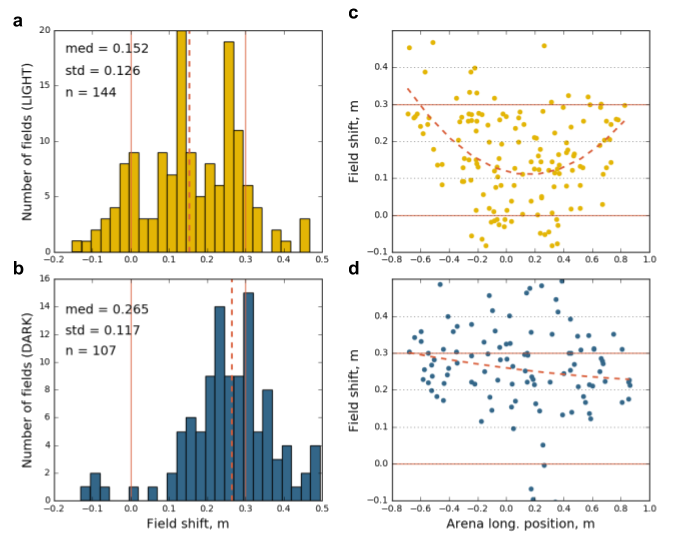
\includegraphics[width=150mm]{figures/F20_light_versus_dark.png}}
\caption[Place fields in light and in dark]{
Change in place field shift distribution for the vSHIFT-physical experiment between light and dark conditions. (a) Distribution of place field shifts in light. Similar to Figure 18a. (b) Distribution of place field shifts in the dark shows that most of the cells rely on path integration in absence of visual input (average shift near 0.3m). Distribution of the place fields of different types inside the arena in light (c) and in dark (d) confirms higher concentration of the visually-driven cells away from the arena boundaries (see next section).
}
\label{fig:F20_light_versus_dark}
\end{figure}

Overall, the dark period is characterized by the reduction in the mean firing rate (by 10\% average, t(146)=-4.38, p<.00002) and decrease in sparsity (by average 15\%, t(146)=-7.85, p<.00001). This might be explained that the loss of visual input, that decreases the overall amount of incoming excitatory activity to the hippocampal circuit, also leads to the reduction in the spiking probability of the place cells in the pyramidal layer. The overall increase in information content (by average 9\%, t(146)=5.21, p<.00001) might be explained by the increased proportion of fields near the boundaries in darkness which are in general more precise (see fine position calibration near the boundaries).

Looking at the place field maps and visually analysing changes of the field locations and place cell activity between light and dark conditions a number of typical cases show up: a) place field firing is completely abolished (see Figure 21a), place field stays in the same location with no substantial change in firing rate (see Figure 21b), place field loses spatial selectivity, changes its firing rate or remaps to a new location within the arena (see Figure 21c). For a more detailed analysis, we separate the resulting fields in 4 groups using the field matching procedure (same as for vSHIFT - coherent, see place field shift detection). If a field $F_a$ has a corresponding field $F_a^{dark}$ in dark, as well as its corresponding field $F_b$ has a pair $F_b^{dark}$ in dark we classify this field as “stable” - these fields keep firing along the whole session in corresponding light and dark periods. If we cannot detect a corresponding pair field in dark condition for either $F_a$ or $F_b$ , we classify this as “B-stable” or “A-stable” field, respectively. If neither of the fields $F_a$ or $F_b$ have a corresponding pair after the lights were turned off we classify this field F as “remapping”.

\begin{figure}
\captionsetup{format=plain}
\makebox[\textwidth]{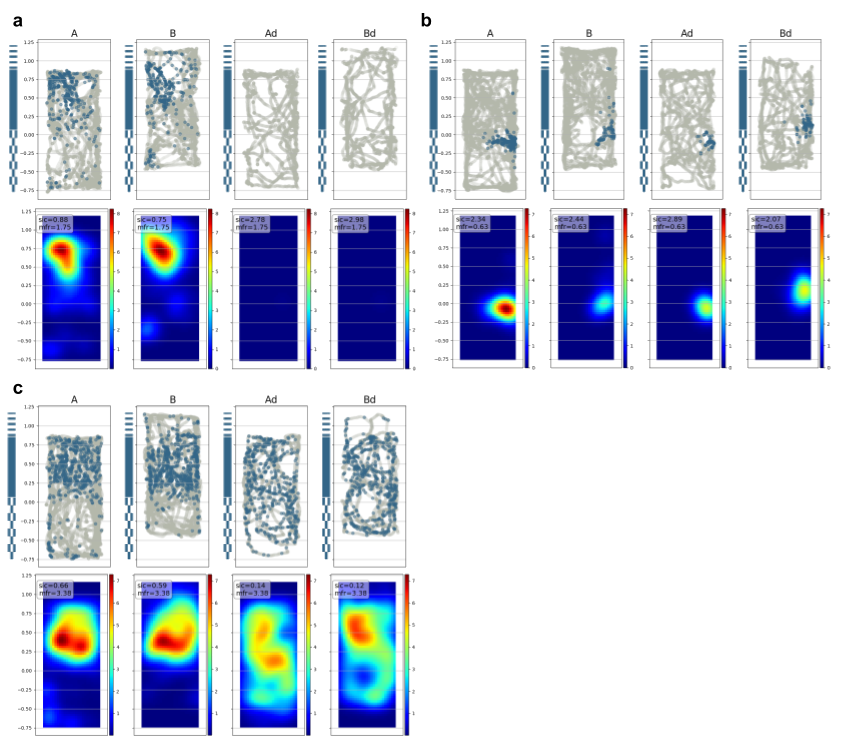
\includegraphics[width=150mm]{figures/F21_remapping_types.png}}
\caption[Remapping in darkness]{
Different types of changes in place cell behavior after the lights are off. (a) An example place cell that goes fully silent in dark. (b) An example place cell with stable location and mean firing rate between light and dark condition shows independence of the visual reference frame. (c) An example cell showing preference for a particular visual part of the environment exposes complete remapping in dark.
}
\label{fig:F21_remapping_types}
\end{figure}

A bit more than a half of the population of fields goes to the stable group (see Figure 21a). Their stability might be due to these cells getting strong self-motion inputs which do not reduce their sharpness (\cite{Allen2016}) and which enable them to keep their stability in darkness. The unstable group, comprising partially stable (place field can’t be detected in both original and shifted positions in dark) and fully remapped fields, react by a significant amount of change to the loss of the visual input and the virtual reference frame.  The contrast between the groups is of  particular interest for investigation relative to their shift preference, which could be attributed to the amount of allocentric and idiothetic information that drive their activity.

The place field shift distribution for the stable group contains a substantial amount of field shifts centered at 0.15 and at 0.3, which correlates with the assumption that these fields are mostly self-motion / boundary-driven and the underlying place cells receive a strong input of information from the self-motion (see Figure 22a). In contrast, all cells in unstable groups are balanced towards 0.0m shift, having field shifts centered at 0.0m and 0.15m and less around 0.3m. This distribution could be explained by assuming that many place fields, driven by visual allocentric information (field shift around 0.0m), when they lose their main driving input, remap or go unstable, thus belong to unstable groups. The correlation between the amount of self-motion input and cell firing stability can be also illustrated by the normalized difference of these field shift distributions (see Figure 22e), which shows negative peak around 0.0m (unstable fields having 0.0m field shift) and positive around 0.3m (more stable field shifts near 0.3m), putatively separating the groups to mostly allocentric- and mostly idiothetic- driven units. Besides field shifts, there is no significant change in mean firing rates for the stable but not for the unstable groups, accordingly. The reduction in mean firing rate might be explained by the loss of visual inputs.

\begin{figure}
\captionsetup{format=plain}
\makebox[\textwidth]{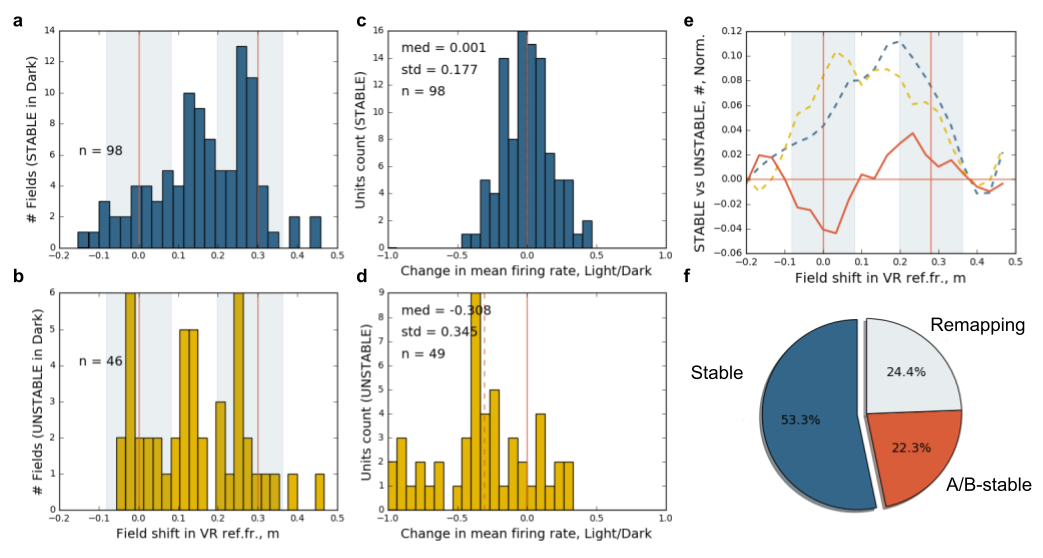
\includegraphics[width=150mm]{figures/F22_stable_unstable.png}}
\caption[Stability explained by self-motion inputs]{
The stability of the cell activity in darkness is correlated with the balance between its visual and self-motion afferents. Distribution of the place field shift (a-b) and change in mean firing rate (c-d) for the stable (cell continues to fire in darkness, top row) and unstable (cell remaps in dark, bottom row) groups. Note that significant reduction in mean firing rate for the unstable group (bottom right) suggests dependency of these cells on the visual inputs. (e) Difference between normalized distributions of place field shifts between stable and unstable groups. The plot shows more visually-driven fields (0m-shift) go to the unstable group, while more self-motion fields (0.3m-shift) go to the stable group, showing a correlation between an amount of shift in light (dependency on the visual reference frame) and firing stability in darkness. (f) Overall classification of all place fields into 3 categories by their stability between light and dark conditions.
}
\label{fig:F22_stable_unstable}
\end{figure}

More intriguing result shows up when analysing the change in place field shift distribution of the stable group between the light and dark conditions. The 0.3m boundary-driven group, assumed to be composed of units mostly driven by self-motion inputs, does not show any change in its shift preference (see Figure 23a, stars). The group of fields near 0.0m, putatively mostly driven by visual cues, loses their 0.0m shift preference and gets a high variance (not shown). Importantly, the middle “multisensory” 0.15m unit group change their shift preference from encoding an average between self-motion and visually given distances (0.15m) to an average shift of 0.3m, indicating the visual input can no longer influence the path integrator for these units and these cells stay driven by the idiothetic inputs only.

Furthermore, the detailed analysis of the place field position shifts for the multisensory 0.15m unit group reveals that in both original and shifted conditions the shift is directed towards the middle between their corresponding place field locations in dark (see Figure 23b). To be more precise, in the original arena position the place field in light is “ahead” of its corresponding field in dark (when it’s self-motion driven only), as the same time for the shifted position the field is “behind” its corresponding field in dark. This direction of the shift is unique to the multisensory group as, for instance, this is not the case for the pure self-motion driven group of cells (see Figure 23c). Altogether this points to the special type of integration of visual with self-motion information. The possible underlying mechanisms are provided in the discussion.

In summary, the change of the place cell firing in darkness confirms the different amount of visual- and self-motion inputs distributed among the 0.0m, 0.15m, and 0.3m shift groups. This suggests the continuous connection between the amount of influence of an allocentric input versus idiothetic inputs and a cell behavior in darkness, ranging from the remapping, if the cell is more visually-driven, to the stable place field in case the self-motion inputs are dominating. The substantial amount of units having 0.15m shift demonstrate the ability of the hippocampal circuitry to use weighted combination of inputs and represent places centered at the average between visual-landmark- and self-motion or boundary-defined distances.

\begin{figure}
\captionsetup{format=plain}
\makebox[\textwidth]{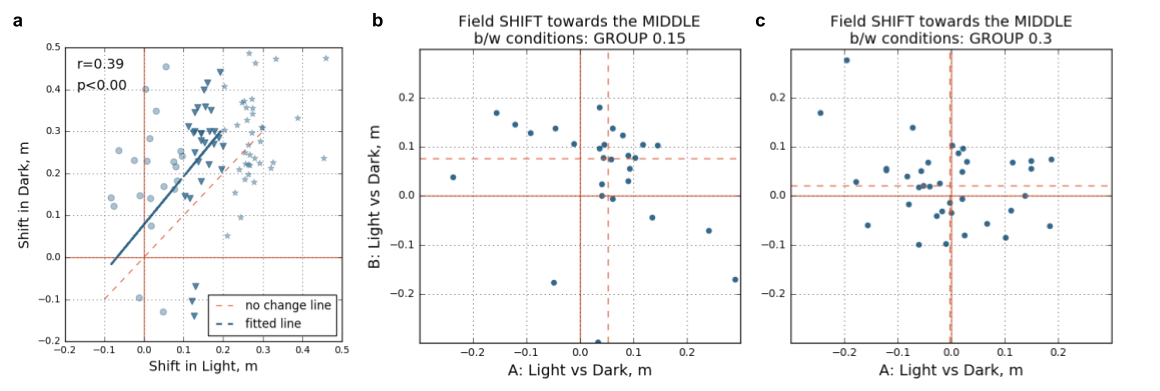
\includegraphics[width=150mm]{figures/F23_shift_to_middle.png}}
\caption[Weigthed combination of the inputs]{
A detailed analysis of place field shifts of the multisensory cells shows the integration of the visual and the self-motion components as a weighted combination. (a) For the stable group, the plot shows place field shift in light versus shift in dark. For the 0.3m fields (stars) place field shift is not different between conditions showing their independence from the visual reference frame. Note that the 0.15m group (triangles) the shift in dark grows to 0.3m showing a switch to the purely self-motion based navigation. (b) Relative shifts in the same arena positions for the 0.15m group show that visual information calibrates the spatial representation towards the middle between the reference frames. For the 0.3m group (c) relative shifts in the same arena positions are not significant probably because of visual independance (right plot).
}
\label{fig:F23_shift_to_middle}
\end{figure}


\section{Fine position calibration near the environmental boundaries}
\label{sec:fine_position_calib}

In the vSHIFT - physical experiment the distribution of place field sizes relative to their arena locations points to a more precise (smaller fields) place encoding near the arena boundaries, rather than in the center of the arena (larger fields, Figure 24a). One explanation of the observed effect might be due to the cells that are getting self-motion inputs tend to be less precise away from the boundaries due to error accumulation in the underlying path integration (\cite{Etienne1996}). Cells closer to the boundaries can easier reset their self-motion dependent component due to the wall proximity, thus being able to more precisely encode actual location. However, this could be also attributed to the increased sensory information due to the direct contact with boundaries (boundary cells). This change in field size, converted to position encoding reliability, was used in the study demonstrating bayesian inference for position encoding by the hippocampal place cells (\cite{Madl2014}).

\begin{figure}
\captionsetup{format=plain}
\makebox[\textwidth]{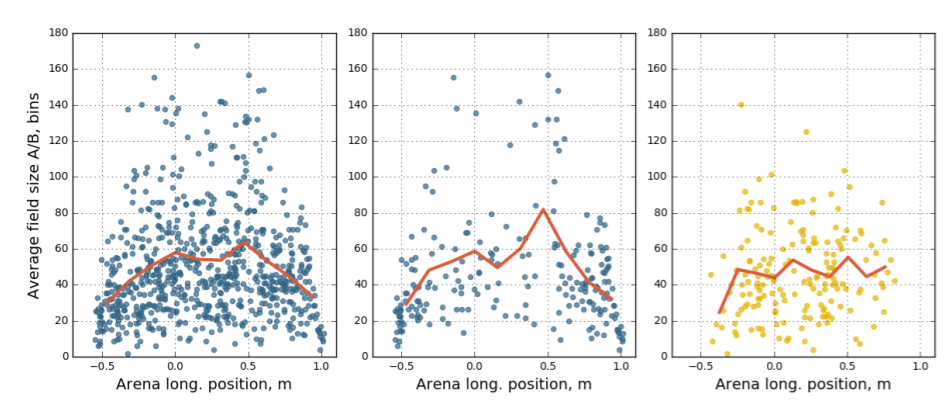
\includegraphics[width=150mm]{figures/F24_field_sizes.png}}
\caption[Position accuracy based on fields sizes]{
The distribution of place field sizes inside the arena. All place fields (left plot) and two groups of self-motion (middle) and visually (right plot) driven fields, classified as in vSHIFT -physical. Smaller sizes of place fields near the boundaries suggest higher quality of spatial orientation.
}
\label{fig:F24_field_sizes}
\end{figure}


%\section{Conflict induced by physical arena translation is comparable to the translation of the visual reference frame}
\section[Conflict induced by visual versus physical translation]{Conflict induced by physical arena translation is comparable to the translation of the visual reference frame%
              \sectionmark{Conflict induced by visual versus physical translation}}
\sectionmark{Conflict induced by visual versus physical translation}
\label{sec:visual_physical_equal}

In order to verify whether the information about the passive move during arena translation and the propagation of this information to the brain circuits through vestibular system is required for the successful encoding of either of the visual- or boundary- reference frames, we conducted visual shift experiment (vSHIFT - visual, Figure 25a). The protocol for the visual shift experiment was exactly matching the physical shift experiment, with the only difference that instead of the arena move for 0.3m, the visual projection was moved 0.3m keeping the same speed, such that from inside the arena the only possibility to distinguish whether the physical arena or the virtual projection is moved is to attend to the vestibular system informing about the start and the end of the passive move, or possibly to the tactile receptors informing about the vibrations during the physical arena move (Figure 25a).

In total 209 place fields were recorded in visual shift condition. Analysis of the place field shift distribution demonstrates presence of field shifts around 0.0m, 0.15m and 0.3m, showing the ability to use both visual and boundary defined reference frames for position encoding (see Figure 25c). High concentration of field shift in the middle of the distribution near 0.15m confirms the tendency of the hippocampal cells to encode the location centered at average between the visual and boundary defined estimates, similar to the physical arena shift condition. The comparison of the place field shift probability distributions between the physical and visual experiments (Figure 25d) demonstrates that even without the vestibular or tactile information about the passive move the visual information alone, when stable for at least 30s periods of time, can influence the positioning of the place fields and overall has very similar impact on formation of the hippocampal place code.

\begin{figure}
\captionsetup{format=plain}
\makebox[\textwidth]{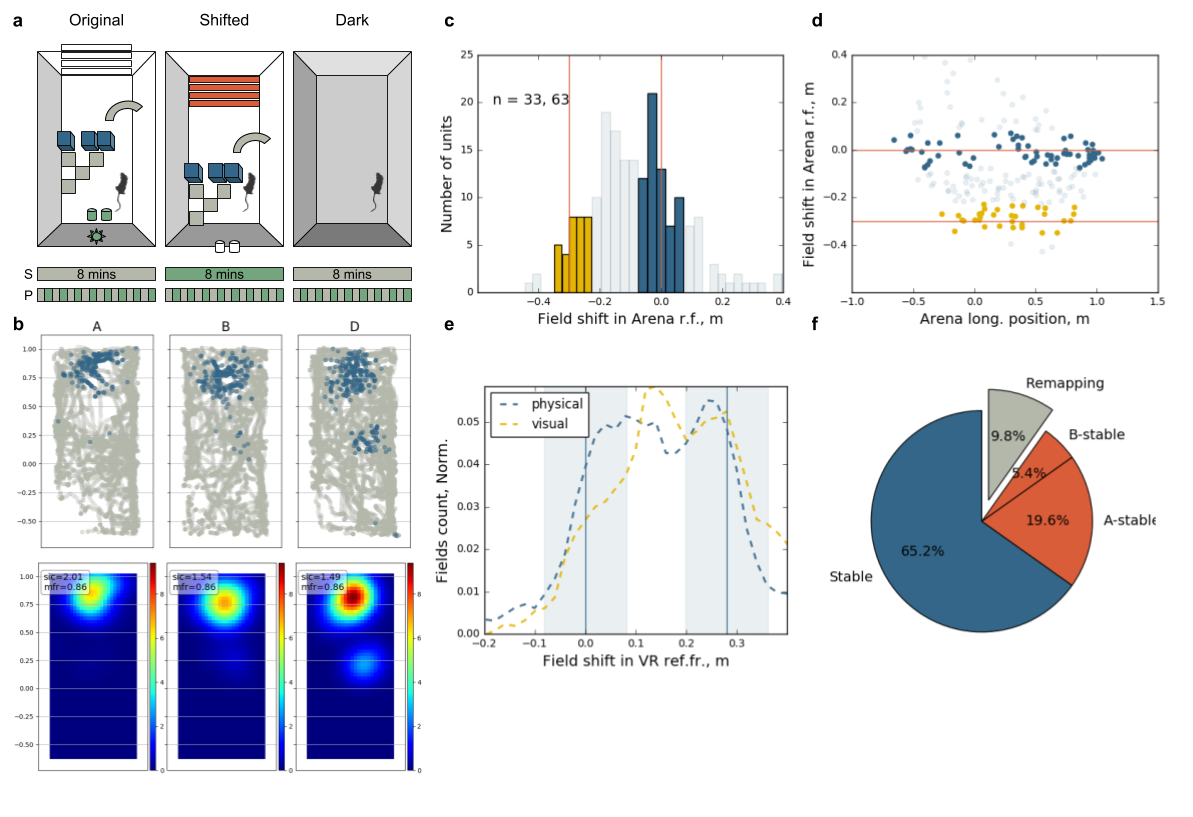
\includegraphics[width=150mm]{figures/F25_visual_equals_physical.png}}
\caption[Visual shift induces sensory conflict]{
vSHIFT-visual. (a) Schematic of the experimental protocol. (b) Example place cell spiking (top) and firing rate maps (bottom) for original, shifted and dark conditions. (c) Distribution of place field shifts is similar to the vSHIFT-physical experiment. (d) Same as in the vSHIFT-physical, there is a higher concentration of the visually-driven fields in the center of the arena, confirming the tendency to rely on the more available reference frame at the population level. (e) Comparison of normalized place field shift distributions between physical (arena moves) and visual (projection moves) types of experiments. (f) A substantial (90.2\%) amount of cells continue to be active in the dark showing widespread integration of the self-motion component.
}
\label{fig:F25_visual_equals_physical}
\end{figure}


\section{Visual conflict induces recalibration of the self-motion based place map}
\label{sec:recalibration}

Similar to the vSHIFT-physical, for several sessions in vSHIFT-visual we recorded navigation in the dark after the shifted condition. This allowed us to analyze the contribution of the induced visual mismatch to the self-motion based representation of the environment. At first, as many place cells integrate both self-motion and visual inputs, we assumed that turning the light off after “shifted” (B) condition would just cut off the visual part and bring the overall place representation into the “original” (A) learned state. In other words, for place fields that are active in dark we expect that place field would shift back to match the original position in A, because of the loss of the visual influence.

\begin{figure}
\captionsetup{format=plain}
\makebox[\textwidth]{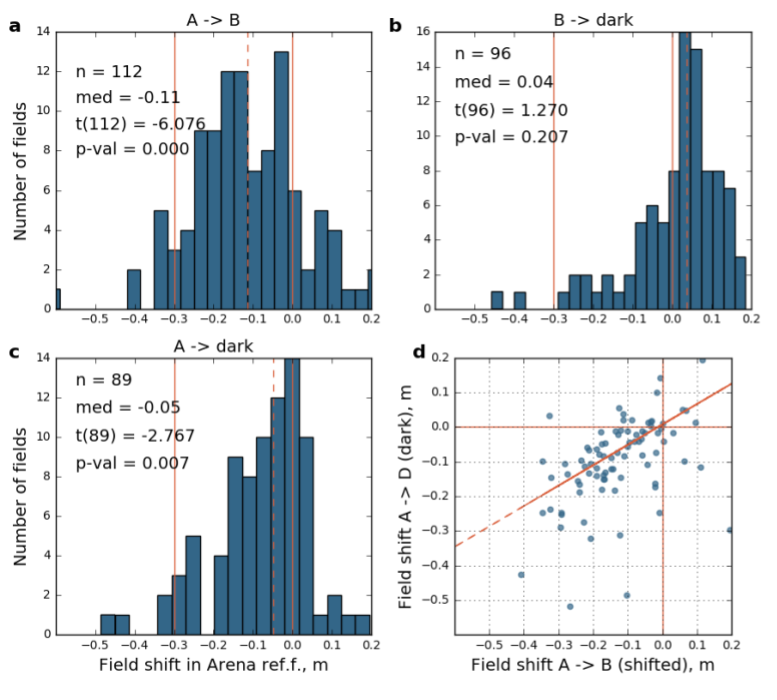
\includegraphics[width=110mm]{figures/F26_recalibration.png}}
\caption[Recalibration of the self-motion map]{
Visual conflict induces recalibration of the idiothetic self-motion based place map. (a) Distribution of the place field shift in light (A -> B) shows the influence of the conflicting visual reference frame and suggests encoding in a weighted combination manner. (b) a very little place field shift back after the lights are off (non-significant) shows that the overall spatial representation was recalibrated during conflicting condition. (c) Direct comparison of original (A) and dark (D) conditions confirms the recalibration of the spatial map as in (b). (d) A correlation between the field shift in light (e.g. its dependency on vision) and the resulting shift of the field (A -> Dark) demonstrates the connection between the amount of visual input and its influence on recalibration.
}
\label{fig:F26_recalibration}
\end{figure}

Surprisingly, this appears not to happen. As described in the previous chapter, on the population level there is indeed a place fields shift between original A and shifted B conditions (Figure 26a, n is smaller comparing to 25c as only sessions with dark periods are taken into account) due to the conflict induced by a shifted visual reference frame (by -0.11m average, t(112)=-6.07, p<.00002, Figure 26a). However, the shift “back” to the original representation is not significant (0.04m average, t(96)=1.27, p=0.2, Figure 26b). The same is confirmed by looking at the place field shift distribution between original A and dark D conditions (-0.05m average, t(89)=-2.76, p=0.007, Figure 26c). Taking individual fields and their shift induced by a visual-to-self-motion conflict versus the shift between original condition and darkness one can see, that cells that have a larger shift in conflicting conditions (more influenced by vision) tend to recalibrate more relative to their original position (Figure 26d). The interference of two reference frames led to a new state of the spatial map, where place code represents the weighted combination of them.

The results demonstrate that the self-motion based and visual landmark-based spatial representations are interconnected. Conflict induced by the shifted visual reference frame leads to recalibration of the whole spatial representation system, including the self-motion based representation. How can the change in place representation in the upstream CA1 area influence the self-motion based representation, located hypothetically in the downstream cortical areas (e.g. head-direction, speed, grid cells)? Theoretically, this recalibration could be implemented via backprojections from the hippocampal CA1 to the entorhinal system via subicular pathways. This has been already hypothesized and similar results were collected in the modelling study (\cite{Li2020}).


%\section{Gradual mismatch between sensory inputs confirms weighted position estimation at smaller conflicts}
\section[Weighted position estimation at smaller sensory conflicts]{Gradual mismatch between sensory inputs confirms weighted position estimation at smaller conflicts%
              \sectionmark{Weighted position estimation at smaller sensory conflicts}}
\sectionmark{Weighted position estimation at smaller sensory conflicts}
\label{sec:gain_12}

To further investigate the change in spatial selectivity of hippocampal cells in an continuously growing sensory conflict we designed an experiment with gradually increasing mismatch between position estimations coming from two different reference frames. By inducing a visual to self-motion instantaneous gain difference along the longest dimension of the arena in an asymmetric way we assume that the gain mismatch between self-motion and visual flow would affect path integration, providing a way to test its contribution to the CA1 place code, as well as allowing to test whether place fields would gradually follow the mismatch estimating position as a weighted combination of both types of sensory inputs.

\begin{figure}
\captionsetup{format=plain}
\makebox[\textwidth]{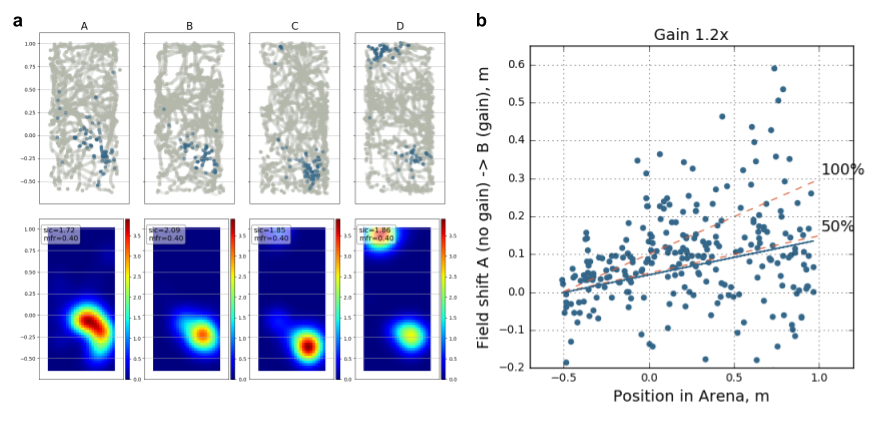
\includegraphics[width=150mm]{figures/F27_gain_12x.png}}
\caption[Sensory integration in gradual mismatch in vGAIN 1.2x]{
vGAIN 1.2x experiment. (a) An example place cell with a field active in all conditions. The gradual shift of the field along the shift of the visual reference frame (north -> south) shows influence of visual objects and cues. (b) Place field shifts between no-gain (A) and gain (B) conditions plotted against  the position in the arena. Dashed lines indicate the amount of conflict between visual and boundary-defined reference frames (100\% reflects the amount of conflict at the Y-axis). Note neurons encode the weighted average between two reference frames (blue linear regression bar), that linearly grows with the amount of conflict, on the population level.
}
\label{fig:F27_gain_12x}
\end{figure}

In the first phase (A) of the vGAIN experimental session animals were learning the stable virtual environment, coherent with environmental borders. The slow transition to the vGAIN 1.2x phase (B) introduced a visual to boundary-defined conflict in self-location ranging from no conflict near the southern arena wall to the 0.3m conflict near the northern arena wall. In line with previous vSHIFT experiments, we expect no place field shift at the southern wall followed by a gradual increase in the shift towards the northern arena wall up to a 0.3m, when comparing the initial (no-gain) and gain conditions.

In total, 275, 316 and 253 place fields from 4 animals were recorded in the vGAIN 1.2x experiment for each condition (no gain - gain - no gain shifted), respectively. An example place field, showing an influence of the conflicting visual inputs is presented in Figure 27a. Although we encounter a variance of place field shifts for different parts of the arena between no-gain and gain conditions, on the population level, we see that there is a gradual influence of the visual- to self-motion conflict along the arena, as expected. Specifically, cells tend to encode the average between the estimations given by two conflicting reference frames, positively correlated with the gradually increasing conflict (Figure 27b), providing more evidence for the hypothesis regarding the weighted combination of sensory inputs by hippocampal cells.


\section{Abandonment of a sensory estimate at larger sensory conflicts}
\label{sec:gain_12}

It has been shown for different sensory modalities and different animal species and also humans, that information from the internal body and environmental cues are integrated at small sensory conflicts to increase response precision (see Optimal combination of environmental cues). However, as proposed in several studies, it is reasonable to abandon less reliable sensory input in case of large conflicts  (\cite{Sjolund2018}; \cite{Cheng2007}). To test whether there is a change in place cells behaviour at larger conflicts we conducted an asymmetric vGAIN 1.4x experiment following the same vGAIN protocol, which enabled to record 1.4 gain mismatch between vision and self-motion, as well as to analyze the gradual increase of conflicting position estimation ranging from 0 to 0.6m.

Similar to the vGAIN 1.2x, the first, exploratory phase, followed by a gain condition where we induced an asymmetric 1.4x gain between self-motion and visual flow. The asymmetry enabled it to build a gradual conflict along the arena, from northern (0 conflict) to southern (0.6m conflict) wall. Taking into account an average place field size of 0.42m within these experimental conditions, the smaller gain of 1.2x and the conflict of 0.3m would still keep the incoming pre-synaptic inputs, defined by different reference frames, overlap, potentially bringing a situation to a smaller sensory conflict category, where the integration of sensory inputs makes sense. In contrast, the gain of 1.4x would build larger conflicts exceeding the average place field size, making self-motion and visual inputs completely uncorrelated in space and time. This conflicting condition might bring many place fields to the larger conflict category, where it makes sense to abandon one of the inputs. In that case, we would expect cells to prefer self-motion or path integration relative to the visual cues, as reported previously for human and rat studies (\cite{Sjolund2018}; \cite{Zhao2015}; \cite{Shettleworth2005}).

\begin{figure}
\captionsetup{format=plain}
\makebox[\textwidth]{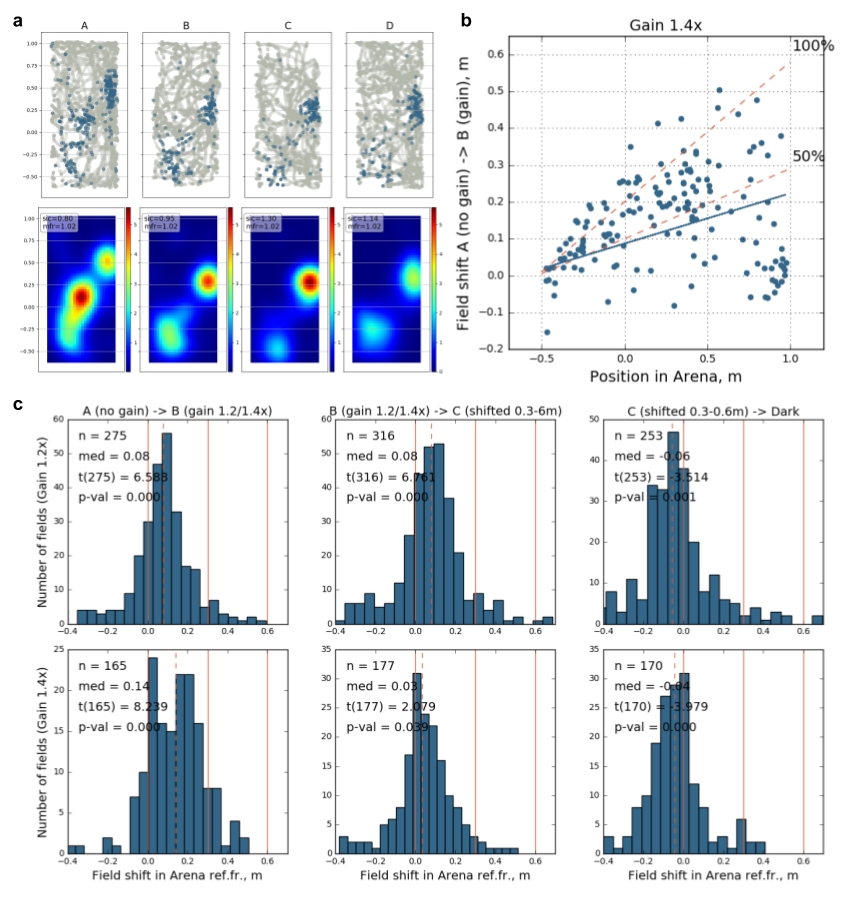
\includegraphics[width=150mm]{figures/F28_gain_14x.png}}
\caption[Sensory alternation in gradual mismatch in vGAIN 1.4x]{
vGAIN 1.4x and analysis of GAIN experiments. (a) An example place cell with a field active in all conditions. The gradual shift of the field along the shift of the visual reference frame (north -> south) shows influence of visual objects and cues. Note that in contrast to the gain 1.2x condition, a field is no longer influenced by vision when conflict is too large (B -> C). (b) Place field shifts between no-gain (A) and gain (B) conditions plotted against  the position in the arena. Dashed lines indicate the amount of conflict between visual and boundary-defined reference frames (100\% reflects the amount of conflict at the Y-axis). Note neurons encode the weighted average between two reference frames (blue linear regression bar), that linearly grows with the amount of conflict, until the conflict does not exceed ~0.4m. At larger conflicts > 0.4m there is a significant drop in the fraction of cells influenced by the visual reference frame. (c) Distribution of place field shifts for no gain (A) - gain (B) and gain (B) - no gain shifted (C) conditions shows continuous influence of the visual reference frame at smaller conflicts, similar to the vSHIFT experiment (top row, left and middle). A small shift back after the lights are off (top right plot) shows the overall recalibration of the spatial map between original and shifted conditions, similar to vSHIFT - visual. In contrast, the initial influence of the visual reference frame (bottom left) stops when the conflict becomes too large (bottom middle).
}
\label{fig:F28_gain_14x}
\end{figure}

A typical example of the place field shift is shown on Figure 28a. At first, a place field follows the visual projection and shifts in the direction of the conflict, encoding a weighted combination of the estimations (A -> B). However, after we asymmetrically reduce back the gain to no gain condition (B -> C) bringing two reference frames in a larger 0.6m conflict relative to the original condition, the place field tends to ignore further visual shift and keeps its spatial preference relative to the arena boundaries. This ignorance of the visual but not self-motion, or path integration driven spatial preference is confirmed by the stable spatial in darkness after the shifted condition (C -> D).

In total, 165, 177 and 170 place fields from 2 animals were recorded in the vGAIN 1.4x experiment for each condition (no gain - gain - no gain shifted), respectively. On the population level, as expected from the multisensory integration, cells tend to follow the visual reference frame in a weighted combination manner (Figure 28b, left part of the plot) at arena south, where the conflict between reference frames is relatively small (0 - 0.3m). However, at an arena north where the conflict exceeds a certain threshold, there is a decrease in the concentration of place fields following the visual projection in favor of the self-motion, boundary-defined input (Figure 28b, right part of the plot). This would be in line with an assumption, that cells tend to abandon one of the inputs at larger sensory conflicts.

Similar to the vSHIFT - visual experiment, the distributions of the place cell shift for the vGAIN 1.2x show overall shift of 0.17m between original (A) and shifted (C) conditions (e.g. “shift via gain”, Figure 28c top left plots). Interestingly, that turning the lights off at the end of the session led to a significant, but relatively small shift back of the overall spatial representation (Figure 28c top right plot), but not to the original position, which again supports the hypothesis of the recalibration of the self-motion based spatial representation by inducing a visual conflict (see visual conflict induces recalibration of the self-motion based map). For the 1.4x gain, enabling gain with asymmetric conflict leads to an overall significant shift of 0.14m at the population level (Figure 28c bottom left plot), smaller that the average between estimations given two reference frames, probably because cells tend to ignore visual reference frame at larger conflicts at the northern part of the arena. Further conflict from gain to no gain shifted (B -> C) does not have any further influence on the place cell location (Figure 28c bottom middle plot), potentially because of an overall larger conflict between original and shifted conditions (A -> C, 0.6m). Similar to the gain 1.2x, a small shift back is detected after the lights are off (Figure 28c bottom right plot), contributing to the recalibration hypothesis.


\chapter{Materials and Methods}
\label{ch:methods}

\section{Electrophysiology}
\label{sec:ephys}

\subsection{Subjects}

All experiments were conducted with Mongolian gerbils (Meriones unguiculatus). Gerbils were selected as an experimental animal for a number of reasons. First, gerbils were shown to have a good visual acuity (~ 1.75 cycles/deg grating acuity at 70 cd/m2; \cite{Baker1983}) and visual alertness (\cite{Ingle1981}). Second, gerbils are more active in the light part of the day cycle (\cite{Naumov1975}), suitable for experimental recordings. Finally, gerbils show better exploration of novel contexts and less dependency on moving along the boundaries (thigmotaxis) (\cite{STUERMER2003249}), which is highly important to reach high levels of arena occupancy across all experimental conditions.

In total, 9 wild-type animals from the local breeding facility were used. Among those, all 9 were used in the shift experiment, and 4 were recorded in the gain experiments, so some animals took part in both experimental paradigms. After the implantation of microelectrodes, animals were housed individually with a maintenance of the 12 hours light/dark cycle. A few days after the surgery and before the start of the experiments animals had ad libitum access to food and water. During the recordings, animals were kept on a food diet to maintain 90-95\% of their original ad libitum weight to increase the interest in random foraging for food pellets during the recording. All experiments were approved according to national and European guidelines on animal welfare (Reg. von Oberbayern, license number AZ 55.2-1-54-2532-70-2016).


\section{Implant design}
\label{sec:implant_design}

In the beginning, we used 4- or 8-tetrode Axona microdrives (Axona Ltd., U.K. http://www.axona.com/) to record from the dorsal CA1 region of the hippocampus. Later in the project, aimed at increasing the density of the recording sites in the brain area of interest as well as to have a possibility to reuse recording devices we chose the 32- and 64-channel Buzsaki H64 silicon probes as candidates for electrophysiological recordings. In order to support implantation, maintenance and successful recovery of the probe after the end of the experiment, a set of custom components was designed. These include the microdrive, the base plate, the protecting box and a set of components supporting the implantation procedure.

\subsection{Microdrive}

The industrial microdrives (e.g. nano-Drives from Cambridge NeuroTech) are usually very expensive and do not allow reusing the recording device. The recent advances in 3D-printing allowed for custom design of the small components, necessary to build reliable microdrives within a short period of time. To be able to change to the procedure to using silicon probes instead of tetrode drives I designed a custom microdrive that meet the following characteristics:

\begin{itemize}
    \item the bottom size of the microdrive should not exceed 20 $mm^2$ to be able to be cemented on the gerbil skull, as well as the body of the microdrive should be fully contained inside the protecting box
    \item the weight of the microdrive should not exceed 2g to be able to carry by small animals
    \item the smallest stable movement of the shuttle of the microdrive should be in the range of 30 to 50 um
    \item the microdrive should be resistant to vibrations and stable enough to allow up to 24 hours of recordings from the same units
    \item the microdrive can be (partially) recovered together with the recording device to be able to be fully reused in the next implantation
\end{itemize}

\begin{figure}
\captionsetup{format=plain}
\makebox[\textwidth]{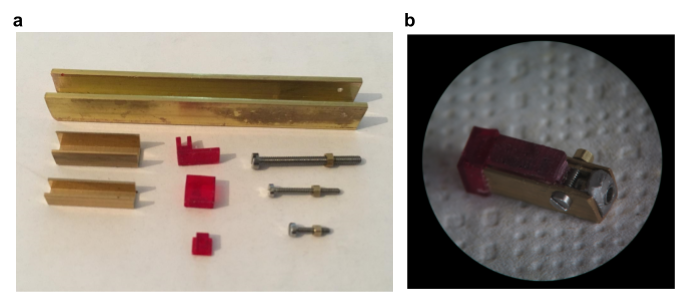
\includegraphics[width=150mm]{figures/F29_microdrive.png}}
\caption[Microdrive]{
Pictures of the custom-made microdrive. (a) 3D-printed and pre-cut brass parts, required to build the microdrive. (b) A picture of the assembled microdrive.
}
\label{fig:F29_microdrive}
\end{figure}

In the beginning of the project, I invested time to design the custom microdrive that meets these criteria (Figure 29 a and b). The major parts needed to assemble the microdrive are the U-shaped rails (commercially available), the M1 and M1.4 10mm screws (also commercially available) and the custom designed plastic parts. The Asiga Pico2 3D printer (https://www.asiga.com/) was used to print the plastic parts. The M1 driving screw having 250um height change per full turn allowed for the 31.25um single movement precision when rotated at 1/8 of a turn per adjustment. The total price of the required parts does not exceed 5 euros, the assemble time does not exceed 1 hour if the printed parts are ready. The drive was successfully implanted to 12 gerbils and proved it’s stability during the recordings. Most of the silicon probes were fully recovered after the end of the experiment, although some had to be trashed due to the surgical issues (recording shanks were clogged by cerebro-spinal fluid or some bleeding and the probe was not recoverable).

\subsection{Protecting box}

In contrast to the different designs of the tetrode drives, which are typically cemented to the skull together with the connector and protection for moving parts, the reusable microdrive with the recording device should be placed in a separate protective enclosure, disconnected from the drive itself. The standard procedure is to build this exclosure from copper mesh during the surgery, gradually building the shielding walls with cement. This method requires careful manipulation of the mesh parts with close proximity to the implanted probe and takes a long time, increasing the duration of the surgery and reducing the chances for successful recovery. The availability of high-precision 3D-printing in house allowed to design a custom protective box that can be assembled directly on the head of the animal during the surgery in a matter of a few minutes (figure 30a). The box has the following properties:

\begin{itemize}
    \item it is fast and easy to assemble during the surgery, easy to dismount at the end of the experiment
    \item it has a quickly removable cover for a) adjustments of electrode’s position, and b) changing the type of the cover from the simple protecting cover to the recording cover that has infra-red sensitive markers, required for tracking system
    \item it’s length and width do not exceed 18x18 mm to not interfere with gerbil eyes and ears position
    \item it is lighter than 3g to not exceed 5g of the total implant weight together with the microdrive
    \item it protects the recording device from dust (while animal is in cage) and light (during recording)
    \item it is strong and can last for long time (up to several months)
\end{itemize}

\begin{figure}
\captionsetup{format=plain}
\makebox[\textwidth]{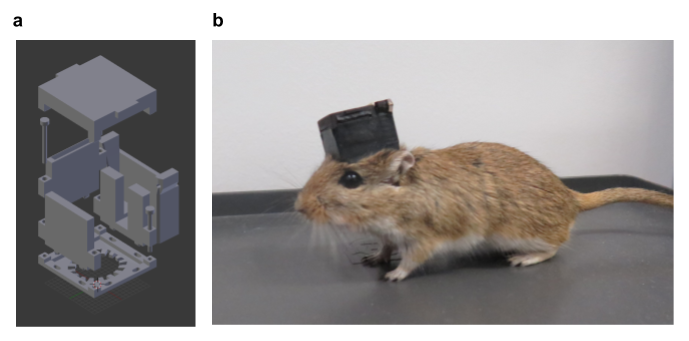
\includegraphics[width=150mm]{figures/F30_crown.png}}
\caption[Protecting box]{
(a) A 3D-model of the protecting box with the connector pocket. (b) A picture of the implant on the animal.
}
\label{fig:F30_crown}
\end{figure}

I designed the corresponding protecting box for 3D printing. I used 1x1.5x5 mm magnets, glued inside both the walls of the box and the top cover, to implement easy access inside for electrode adjustments. The M1 10mm screws were used to hold the walls together. As a result, the overall surgical time decreased and the new implant design allowed for the recovery of the recording device with the connector at the end of the experiment.

The designed protective box was successfully used in 12 animals (figure 30b), 4 of them for the duration of more than 2.5 months. Despite the light accumulation of dust inside the box, due to an imperfect connection between the top cover and the wall with the connector, the box was stable and reliable and didn’t show any failure in all of the animals.


\subsection{Surgery}

Standard stereotaxic surgical procedures of implantation of microelectrodes in the rodent hippocampal area CA1 were performed. Before the surgery, a 3D model prototyping the stages of the implantation was designed to ensure the correct placement of the microdrive and the protecting box, as well as the later fixation of the connector (figure 4.3 a-c). A 3-component solution with medetomidine-midazolam-fentanyl (0.15mg/kg, 7.5mg/kg, 0.03mg/kg) was used to anesthetize animals and keep the anesthesia for the duration of the surgery, by re-injecting the solution every 2 hours if the animal showed foot reflexes. During the surgery, animals were head-fixed in a stereotaxic frame (Stoelting Co.) placed on the heating pad with the termometer to maintain the body temperature of 36°C. All animals were implanted in the right hippocampus. A silicon probe oriented 15\% to the vertical plane attached to a microdrive was inserted into a 2mm wide craniotomy window (AP 3.0mm, ML 3.3mm, DV 0.9mm, averaged using the lambda-bregma distance according to the \cite{Radtke-Schuller2016}). Sealing wax was used to protect the electrodes and to cover the craniotomy window.

\begin{figure}
\captionsetup{format=plain}
\makebox[\textwidth]{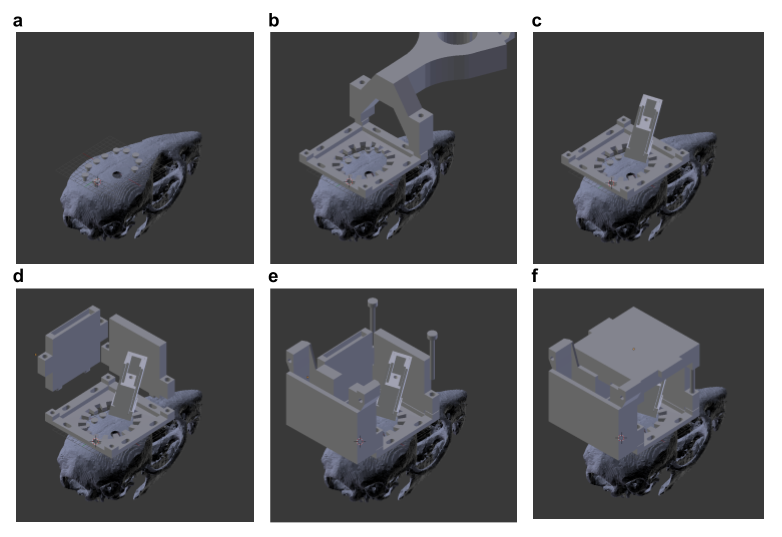
\includegraphics[width=150mm]{figures/F31_surgery.png}}
\caption[Surgical procedures]{
3D-modelled stages of the microdrive insertion and implant assembly during the surgery. (a) Insertion of the grounding screws to the skull. (b) Fixation of the base plate on top of the grounding screws. (c) Placement of the microdrive with the electrodes under the required angle and fixation of the drive with the cement. (d-e) Assembly of the protecting box using M1 10mm screws on top of the base plate. (f) The resulting implant assembled.
}
\label{fig:F31_surgery}
\end{figure}

The base plate, necessary to hold the protecting box, was cemented to the skull together with 10 M1 1mm screws, anchored to the frontal, left parietal and occipital bones (Dental cement, Paladur). Two screws inserted in the occipital bone above the cerebellum served as electrical ground. The surgery finished with the 3-component antagonist atipamezole-flumazenil-naloxone (0.4mg/kg, 0.4mg/kg, 0.5mg/kg). The post-surgical treatment included 5 days of daily injections of antibiotics (Baytril, 10mg/kg) and 3 days of analgesics (meloxicam, 0.2 mg/kg). The recordings started only after complete animal recovery.


\subsection{Recording procedures}

After the successful animal recovery the electrodes were adjusted daily to lower the probe tips with recording channels to the pyramidal layer of hippocampal CA1. Lowering of the electrodes was done in small increments of 1/8 to 1/4 of a turn (31.25 to 62.5um) not exceeding 125um per day to avoid damaging neural tissue and missing the right hippocampal layer. To make a proper adjustment, an animal was connected to the acquisition system before the move of the electrodes and the LFP signal was monitored. The correct placement of the electrodes was defined by several factors, including the presence of sharp waves (\cite{Buzsaki1986}) and ripples (\cite{OKeefe1978}) in the LFP signal during immobility periods, as well as the presence of simultaneous bursts of spikes pointing to the putative pyramidal cell activity in this region. If these factors were not observed within a reasonable time (approx. half an hour) the electrodes were adjusted and an animal was left for another half a day. Otherwise, an experimental session was recorded.


\subsection{Histology}

To confirm the correct electrodes location, a histology on the animal’s brain tissue was performed. Animals were deeply anesthetized with pentobarbital and perfused with 4\% paraformaldehyde. After the perfusion, brains were extracted and stored in paraformaldehyde for at least one day. Brains were sliced coronally in 60um slices and the slices near the craniotomy were stained with neutral red. Pictures of the slices were taken using the 10x microscope (see examples on figure 32).

\begin{figure}
\captionsetup{format=plain}
\makebox[\textwidth]{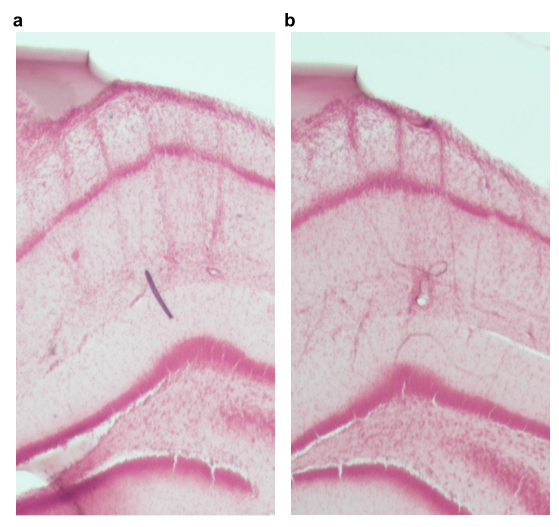
\includegraphics[width=100mm]{figures/F32_histology.png}}
\caption[Histology]{
Example pictures of histological slices. (a) Example picture from animal 00908 slide 6 slice 4 - 2x (b) Example picture from 003281 slide 6 slice 5 - 2x. Note multi-shank tracks of electrodes penetrating the CA1 pyramidal layer (top).
}
\label{fig:F32_histology}
\end{figure}


\section{Virtual reality setup}
\label{sec:vr_setup}

\subsection{RatCAVE system}

All experiments were designed to be conducted in a 3D virtual reality setup named ratCAVE (\cite{DelGrosso2018}). The setup consists of a large rectangular arena (floor area 162 cm × 72 cm and walls of 60 cm height, placed with a 70 degrees angle to accommodate the visual projection),a set of 7 infra-red tracking cameras (Prime 13W 240 fps, OptiTrack, NaturalPoint Inc., United States) located above the arena, and a high-frequency projector (Prime 13W 120 fps, OptiTrack, NaturalPoint Inc., United States), used to project a 3D virtual environment on the walls of the arena. Each experimental session a 3D-printed set of three spherical reflective markers was magnetically attached to the head of the animal, on top of the implant to not interfere with the headstage. These markers were tracked in a closed-loop by the cameras  to be able to adjust the projection depending on the animal's position. Blender (https://www.blender.org/) package was used to design the virtual environment and export it to .obj files, used by the custom-written 3D graphics python software (\cite{Grosso2019}) for rendering.

Two standard linear actuators and a bearing rail system were installed below the arena to physically move the arena ialong one coordinate axis. The maximum move was 30cm, limited by the borders of the projection. The actuators were controlled by an arduino with a motor shield, connected via USB / serial port to the computer with the experiment control software.

\begin{figure}
\captionsetup{format=plain}
\makebox[\textwidth]{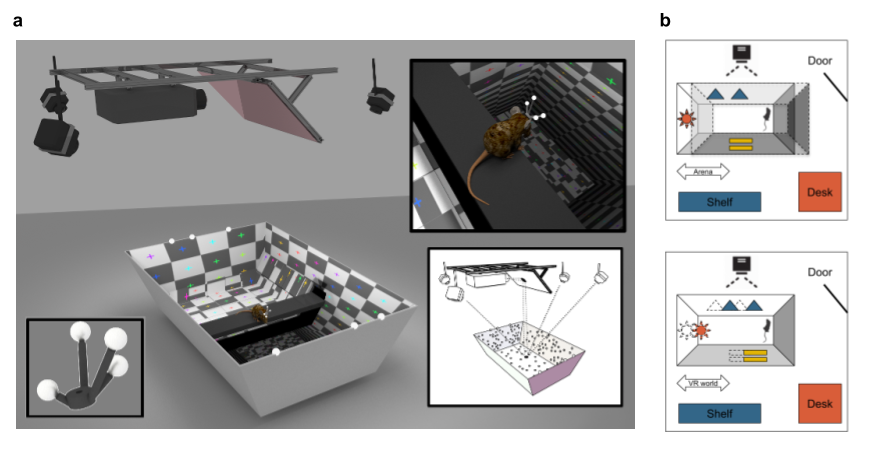
\includegraphics[width=150mm]{figures/F33_VR_setup.png}}
\caption[Virtual Reality Setup]{
The ratCAVE freely-moving virtual reality system for rodents used in experiments. (a) A 3D-model of the arena, position tracking and the projection systems. Left inset (left) shows the reflective markers placed on the animal's head, which is used by the tracking system to locate the animal (adapted from \cite{DelGrosso2018}). (b) Location of the arena in the experimental room and a schematic of the potential experiments: linear translation of the arena using linear actuators (top) or manipulation of the virtual projection (bottom).
}
\label{fig:F33_VR_setup}
\end{figure}


\subsection{Rewarding system}

A food dispenser (Campden Instruments Ltd.), positioned above the arena served for automatic reward administration. As most of the experiments were designed for random foraging, a food dispenser was triggered for dropping a food pellet (20 mg, TestDiet LabTab AIN-76A) at a random location within the arena at 1 minute intervals.


\subsection{Acquisition system}

An Open Ephys acquisition system (www.open-ephys.org , \cite{Siegle2017}) driven by an Opal Kelly XEM-6310 FPGA module was used to acquire neuronal data at a 30kHz sampling rate. The 32 or 64-channel Buzsaki H64 silicon probes were connected via the Intan RHD2000 series headstage to the acquisition box, which transmitted the raw data to the Open Ephys GUI for saving and visualization. The synchronization between the electrophysiology and virtual reality systems was done using the “Network Events” plugin, essentially implemented by periodic sending of TCP packets using python ZeroMQ package from the VR computer to the Open Ephys acquisition socket on the Ephys computer, connected directly via ethernet cable.


\subsection{Automatic experiment control}

A custom experimental control software was written to asynchronously manage the virtual projection, information from the tracking system, linear actuators, food dispenser, visualization of the animal position, video- and position logging and synchronization with the acquisition system. The non-blocking transmission of the information between components was implemented using the PUB/SUB communication scheme based on the ZeroMQ messaging system (https://zeromq.org/). Rendering of the virtual projection was performed by the ratCAVE package (\cite{Grosso2019}), food dispenser and linear actuators were connected and operated via USB serial ports, OpenCV (https://opencv.org/) was used for both video recording and animal position visualization, and built-in python components for metadata and logging.


\section{Data analysis}

Data analysis was primarily done in Python 3.5 with the standard math packages numpy and scipy, as well as scikit-learn, matplotlib and other utility packages. Partially the analysis was done in Matlab R2018b using standard libraries (detection of local minima, detection of center of mass of place fields). Significant amount of analysis was written in Jupyter notebooks for better visualisation. Analysis scripts, jupyter notebooks and the code implementing the data processing workflow are available in the project repository.


\subsection{Data processing workflow}

To increase efficiency and consistency working with large amounts of heterogeneous neuroscience data I developed a custom software automating the data processing workflow. A python package named “stapler” (https://gitlab.lrz.de/asobolev/stapler) was written to implement a pipeline consisting of the following steps:
\begin{itemize}
    \item collecting recording session data about animal positioning, animal electrophysiology and session configuration from the local PCs to the central storage
    \item merging corresponding data into a single folder
    \item converting OpenEphys files to binary formats, creating LFP files, compressing video files
    \item running spike sorting workflow on the raw data (high pass filtering, extracting spikes, PCA on spikes, running KlustaKwik, cleaning up)
    \item backing up unit clusters, syncing position and unit firing data, saving optimized data to HDF5
    \item performing post-processing steps required for final analysis (building place fields, calculate unit metrics, computing center of masses of place fields, running bootstrapping on the spiking data, running density based clustering, calculating place field shift matrixes, creating place field figures for every epoch)
\end{itemize}

The program allowed to change the running configuration for each step independently, enabling having custom processing parameters for different types of experimental sessions.


\subsection{Identification of single units}

Klusta (https://github.com/klusta-team/) software was used to perform spike clustering. The NeuroSuite (http://neurosuite.sourceforge.net/) was used to visualize raw data and to manually filter out noise clusters, as well as to merge similar clusters according to their burstiness and waveform shapes on corresponding channels. Clusters, representing interneurons by their spike width and average firing rate, were not taken into further analysis.
I used cluster isolation distance as a parameter to assess spike sorting quality (\cite{SCHMITZERTORBERT20051}). Clusters having isolation distance < 15 were excluded from further analysis.

\begin{figure}
\captionsetup{format=plain}
\makebox[\textwidth]{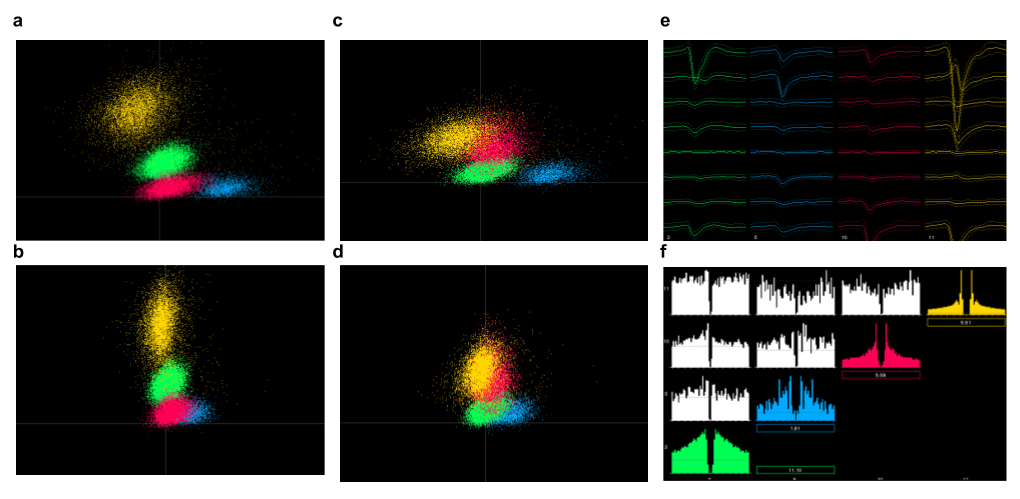
\includegraphics[width=150mm]{figures/F34_spikesorting.png}}
\caption[Spikesorting]{
Spike clustering. (a-d) Example cluster projections in pairs of principal components. Spike belonging to the same cell share the same color. (e) Example waveforms (mean) and (f) cross-correlograms of spiking of the same cells as in (a-d).
}
\label{fig:F34_spikesorting}
\end{figure}


\subsection{Spatial firing maps and place fields}

For every recording session and subsequent experimental condition I calculated spatial firing maps, mainly to visualize the conditional spatial selectivity - the change of the unit firing rate depending on the animal’s and arena position. The space was binned in 0.5 x 0.5 cm squares and the number of spikes for each bin was accumulated. The spiking map was computed by dividing the number of spikes in each square bin by the total time spent in the bin. The resulting firing rate maps were created by applying smoothing with 2D gaussian filter with sigma = 3 cm.

To define the precise analytical locations of place fields, I calculated the areas above the 0.5 * peak firing rate (threshold) of each firing rate map, and each connected area was taken as a putative place field. For each place field the center of mass (COM, Cx; Cy) was calculated:

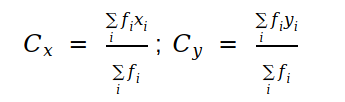
\includegraphics[width=70mm]{assets/formula.png}

where fi  is the firing rate and xi  yi  are the coordinates of the spatial bin. For each place field these centers of masses were not used as a final location of the field but used to further refine the position by bootstrapping.

To reach better precision on defining the place field locations, as well as to exclude noisy fields I used bootstrapping on the original spiking data. First, I split each spike train into several experimental conditions. For each condition I bin the timelapse of the spike train in chunks of 10-15 s and build a new spike train by randomly taking chunks with replacement. As a result of performing this operation 1000 times I get 1000 re-sampled place fields for each experimental condition. Second, for each new re-sampled spike train I compute individual place field locations using the thresholding / center-of-mass method, described above. This resulted in the number of bootstrapped locations of putative place field centers for each unit / condition. By design of the bootstrapping method, the centers of these individual fields tend to cluster together across all resamples if the field is stable, and tend to spread if the field is just noise. To get the actual fields, I used density-based spatial clustering with noise to separate well-connected clusters of bootstrapped field centers. The density-based clustering procedure allows to ignore noisy resamples (less than 100 field centers in the cluster from 1000 resamples), as well as to rank resulting clusters by the number of points (field centers) in the cluster. By taking the clusters with the highest rank I separate the most stable fields from the ones that hardly survive bootstrapping (practically I take the best 2 clusters, e.g taking 2 fields per unit maximum). Finally, the center of each cluster given by the density-based clustering was taken as a final place field location (figure 34 a-c).

\begin{figure}
\captionsetup{format=plain}
\makebox[\textwidth]{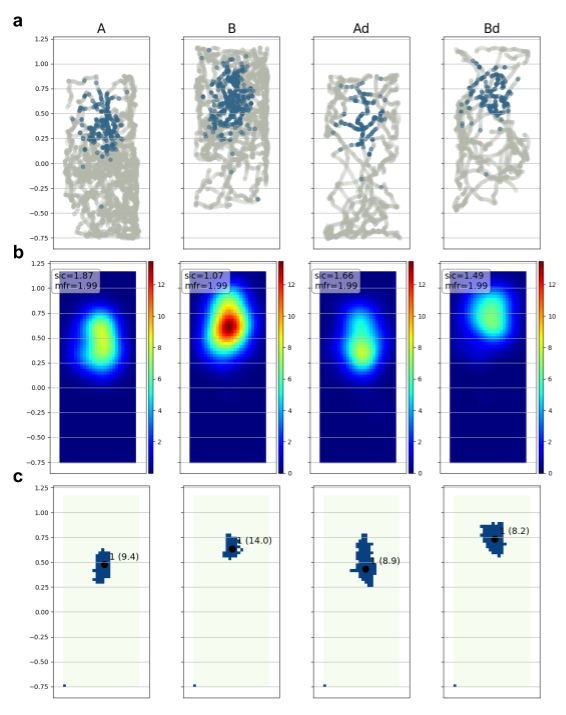
\includegraphics[width=100mm]{figures/F35_place_fields.png}}
\caption[Place field detection]{
Detection of place fields. (a) Example spiking (blue) and arena occupancy (grey) plotted in the arena coordinates. (b) Example firing rate maps of a neuron in (a). (c) Place field patches and their center-of-masses computed using the bootstrapped procedure
}
\label{fig:F35_place_fields}
\end{figure}


\subsection{Place field shift detection}

For each cluster I use it's surface projection to calculate corresponding fields between experimental conditions (Figure 35c). By gradually shifting one projection relative to another in a range from 0 to 0.3 m (the shift of the arena or the virtual projection in all experiments) and computing the maximum of their overlap I determined the clusters which projections overlap the most (if a field in A does not overlap with any other field in B it means it remapped). After the fields are "paired" between conditions the vertical difference between the centers of their clusters (literally center-of-mass of their bootstrapped field centers) is computed as a shift of that particular field between given conditions (Figure 36).

\begin{figure}
\captionsetup{format=plain}
\makebox[\textwidth]{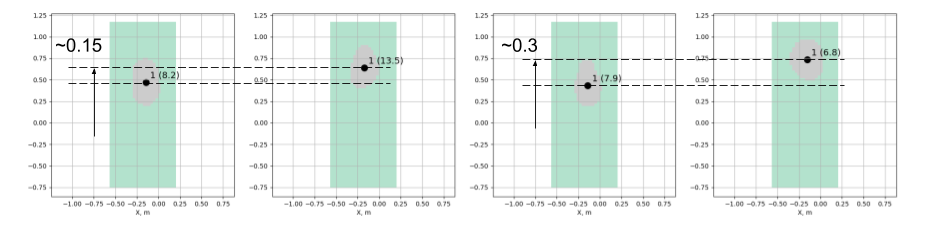
\includegraphics[width=150mm]{figures/F36_shift_detection.png}}
\caption[Field shift detection]{
Detecting place field shift. An example place field with patches in all experimental conditions. This example has only one place field, it has a shift along the Y-axis of 0.15m (light condition, left two plots) and a shift of 0.3m (dark, right two plots).
}
\label{fig:F36_shift_detection}
\end{figure}


\chapter{Discussion}
\label{ch:discussion}

Aimed at contributing to the research on the question of integration of allothetic and idiothetic information at the level of the hippocampal place cells, I used freely-moving virtual reality setup where I conducted several types of electrophysiological experiments with randomly foraging animals. To study the place cell spatial representation I designed vSHIFT, vGAIN and vTELEPORT experiments, each implementing a mismatch between the boundary-defined and the visual reference frames.

From the vSHIFT - coherent experiment we learn that most of the CA1 place cells are getting self-motion inputs. The analysis of the place field shift in the conflicting sensory conditions showed simultaneous encoding of both reference frames, balanced from mostly self-motion driven near the boundaries to the visually driven in the center of the arena. Analysis of the interplay between the visual and self-motion inputs in the vSHIFT experiment confirms better position calibration in the presence of the boundaries versus to the middle of the arena. It was found that, despite previous suggestions that CA1 cells responsive to visual and self-motion cues are anatomically separated (\cite{Fattahi2018}), an evidence that the same CA1 cell can integrate both types of self-motion and visual inputs on the single cell level. These CA1 cells can not only be visually or self-motion selective, but also represent a specific combination of the two types of inputs - forming distinct categories of place fields. Current experiments demonstrate that place cells having self-motion components in their place fields keep being driven by self-motion inputs only, if the visual component is not available. This suggests place cells could use weighted integration of allocentric and idiothetic sensory afferents for spatial encoding.

In the vGAIN experiment, sessions with animals recorded with the 1.2x gain condition showed the strong ability of the hippocampal cells to encode both visual and boundary-defined reference frames even during and after being in conflict between the proprioceptive and visual systems. The distribution of the place fields shifts shows a substantial amount of units having shifts of 0m (visually-driven fields) and 0.3m (boundary driven fields), similar to the regular physical or visual shift experiment. An outstanding amount of fields with the place field shift of 0.15m confirms the above hypothesis of an ability of the hippocampus to represent location as a combination of visual-landmark- and boundary-defined reference frames. Recordings in dark allowed to show that the induced visual- to self-motion conflict results in recalibration of the overall spatial representation, possibly via feedback projections from the hippocampus to the entorhinal cortical areas.

While we collected evidence from both vSHIFT and vGAIN 1.2x experiments that under small conflicts place cells tend to integrate both sensory inputs, the vGAIN 1.4x suggests that in a situation of a larger conflict one sensory modality is being abandoned. Moreover, in line with previous human and animal studies (\cite{Zhao2015}; \cite{Shettleworth2005}), we found that in larger conflicts involving vision path integration tend to be implemented based on non-visual (mostly self-motion, but can be also tactile and olfactory) sensory inputs only; cells mostly encode positions relative to the environmental boundaries, ignoring information coming from vision.


\section{Integration of the self-motion and visual information}
\label{sec:integration_sm_vision}

It is established that hippocampal cells can build spatial representations without self-motion inputs - mainly the grid cell inputs from the entorhinal cortex (\cite{Poucet2015}; \cite{Muessig2015}). Moreover, without the stable grid cell activity new place cells can be established in new environments (\cite{Brandon2014}). This leads to an assumption that both external sensory and internally-generated self-motion information come to the hippocampus as two different, potentially overlapping, parallel pathways - one integrating proprioceptive, vestibular and other idiothetic signals to represent self-motion, another providing a combination of the allocentric sensory signals instantaneously occurring at a particular location.

The data from current experiments demonstrates the reliance of place cells on these inputs via encoding position based either on self-motion, or on visual information, or on combination of both (see results). In contrast to the identified groups of neurons recorded in the body-fixed VR (\cite{Haas2019}), where a negligible subset of neurons shows integrative properties of both allothetic and idiothetic (proprioceptive) inputs, we found a large subset of hippocampal cells being selective based on both types of input. This suggests there is an interference between two input pathways, and involvement of some competitive learning mechanisms used by the hippocampal CA1 neurons to establish their firing preference based on one or another information stream, or a combination of them. This in turn, would suggest a much stronger contribution of self-motion-driven path integration to hippocampal spatial representation than what could be expected from head- or body-fixed VR experiments (\cite{Jayakumar2018}; \cite{Haas2019}; \cite{Chen2013}, \cite{Aronov2014}).

Also, it was long assumed that in absence of boundary-defined reference frame, additional allocentric (e.g. visual) information can “reset” the path integrator, which should move the place field centers such that they have 0m shift and belong to the “visual” group, to represent the position defined solely by the allocentric frame (\cite{Savelli2008}). Instead, our data shows that the information about the moved distance is somehow integrated in the pre-hippocampal brain circuits to represent the average between the distances defined by two different reference frames, and does not simply bind to one or another, at least at small conflicts (see results about removal of a visual reference frame).


\section{Representation of a combination of different reference frames}
\label{sec:integration_two_frames}

Clear effect of visual influence on multisensory boundary-and-visual cells shows that the pure boundary vector cell model (\cite{Barry2006}; \cite{Grieves2018}) or different periodic grid cells inputs (\cite{OKeefe2005}; \cite{Rolls2006}) is not highly probable. The recent work involving single-cell recordings, where place fields can be induced by precise time stimulation (\cite{Zhao2020}), demonstrates that co-firing, or general synaptic plasticity should be a mechanism for recruitment of particular CA1 cells to integrate visual, boundary or multimodal inputs and form a field of a certain type. Another work shows that dendritic plateau potentials, coming from the EC3 in conjunction with CA3, are sufficient to produce place field in CA1 pyramidal cells by means of strengthening synaptic inputs active around the time of plateau formation (\cite{Bittner2015}). Altogether this is a strong evidence for the crucial role of synaptic plasticity in integration of allothetic and idiothetic inputs. Below I would like to propose a few mechanisms how it could be involved in the process of coding an intermediate estimate of the positions, defined by two reference frames.


\subsection{Effect of a shift of a particular reference frame after learning and establishing a place field}

One possible explanation how the average between visual- and boundary-defined distances could be implemented by the hippocampal neurons would be to assume that pyramidal cells, having these fields, receive both inputs from the self-motion (distance from arena walls) and visual (distance to proximal virtual cues) streams. At the time of original field formation, the corresponding sensory and path integrator signals are coherently coming as inputs to the pyramidal neurons to form a stable place field, defined by mutual presence of information about the distance to the walls and information about visual landmarks. This could be done by strengthening the necessary synaptic connections between the appropriate sensory afferents and a particular post-synaptic neuron, encoding this place field. In the shifted condition, signals from the path integrator and a visual system might loose their coherence and appear to be shifted relative to each other in space (Figure 37), leading to the asynchrony in the incoming cell firing and to a shift of the place field center to a half distance between the original position and actual arena shift. If this is the case, this would lead to different place field characteristics between the original and the shifted conditions. If incoming signals are not coherent and have only partial overlap, this should decrease the place field peak firing rate in case of the additive synapses. Also the place field should appear to be larger, as one of the inputs starts to be active earlier (later).

\begin{figure}
\captionsetup{format=plain}
\makebox[\textwidth]{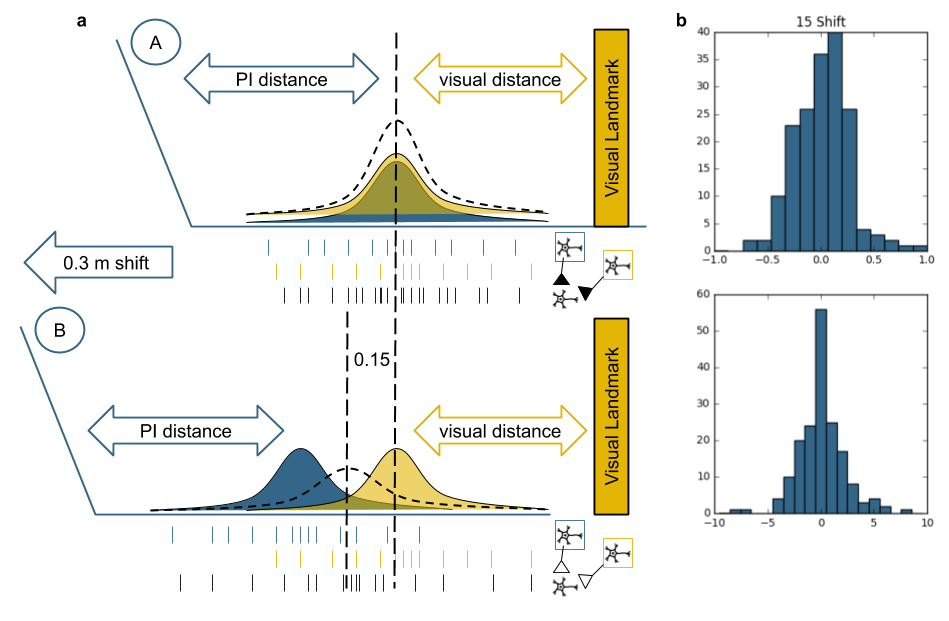
\includegraphics[width=150mm]{figures/F37_encoding_average.png}}
\caption[Encoding average]{
Weighted integration of visual and self-motion inputs might lead to the average representation of the resulting position estimate. (a) Schematic of the inputs to the postsynaptic CA1 neuron. Visual (yellow) and self-motion (blue) afferent estimations are learned in a coherent representation by some CA1 neuron (top row). In a conflicting situation incoming inputs are not aligned which can lead to the averaging of the inputs if the cell is using weighted input integration. Applicable if the conflict is small (place fields overlap). (b) No change in mean firing rate (top plot) and field size (bottom plot) between original and shifted (conflicting) conditions for the group of cells showing average position encoding.
}
\label{fig:F37_encoding_average}
\end{figure}

I verified whether on average place fields in this middle group (0.15m place field shit +- 1 SD of 0.082m) change their firing characteristics between two conditions. Although some of the cells demonstrate exactly these effects (not shown), the total majority of the fields in this group keep their firing rate and field size stable between original and shifted conditions (see Figure 37b). This suggests that either the synaptic connections are multiplicative, or in general there is another mechanism how the average location between points in two reference frames can be represented. One of the opportunities for further investigations is to use the advantage of the VR system and record these groups of cells’ activity when first one and then the other inputs are completely removed.


\subsection{Change in input reliability together with Bayesian coding may explain categorization of CA1 cells by input preference}

According to the principles of optimal Bayesian coding (\cite{Pouget2003}) the weighted integration of sensory estimates should have weights proportional to the reliability of the estimate, in order to maximize the resulting estimate. Intuitively, the reliability of the position estimation relative to the boundaries is highest near the walls (supported by tactile contact) and lowest in the arena center. At the same time position estimation relative to both proximal and distal visual cues and landmarks is almost the same everywhere in the arena except at the actual arena walls, where the quality of the projection is low. If CA1 neurons use weighted integration, having these assumptions a Bayesian estimations integration model (like used in the seminal study by \cite{Ernst2002}) can explain the continuous distribution of place field shifts recorded in the vSHIFT experiments (Figure 38).

\begin{figure}
\captionsetup{format=plain}
\makebox[\textwidth]{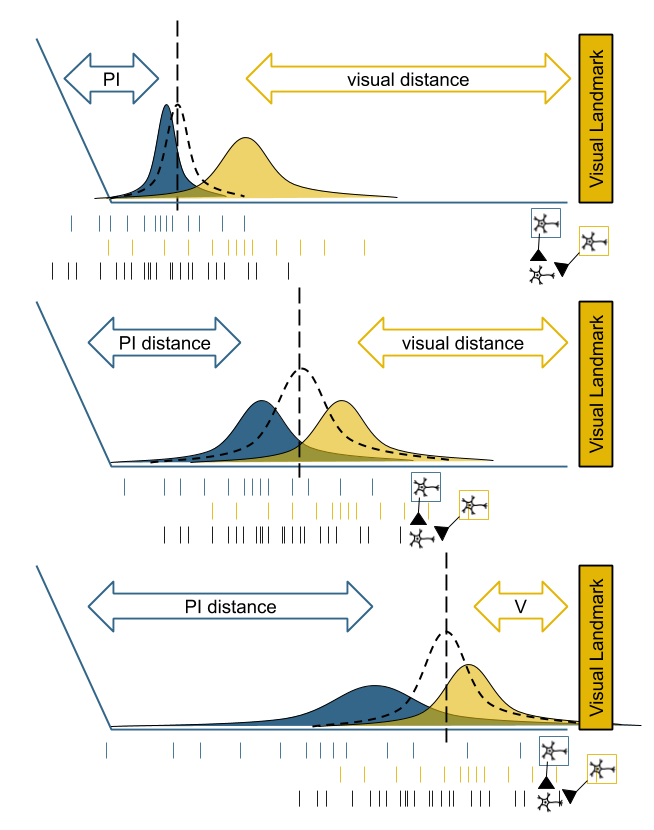
\includegraphics[width=100mm]{figures/F38_weighted_integration.png}}
\caption[Weighted integration]{
Conflicting presynaptic inputs in different places within the arena together with Bayesian coding can lead to formation of all categories of visually and self-motion driven place cells. (top) High reliability of the self-motion inputs near the boundaries results in formation of self-motion driven place cells. (middle) Relatively equal contribution of both types of sensory inputs leads to formation of cells encoding average between reference frames. (bottom) Higher reliability of the visual signals away from the boundaries results in formation of visually-driven place cells.
}
\label{fig:F38_weighted_integration}
\end{figure}

In particular, one can assume that indirect EC2 inputs to the hippocampus e.g. to the area CA3 might lead to the existence of two different continuous attractor networks, each encoding position relative to a different reference frame (\cite{Li2020}, \cite{Haas2019}). Then instead of classifying CA1 cells in different groups we hypothesize all cells use the same principles of sensory integration (near-like optimal), with the difference that some cells initially by chance are more strongly connected (e.g. via schaffer collaterals) with the neurons from the attractor encoding position based on self-motion, and some with the attractor encoding position based on visual inputs. This assumption can also explain why there is a balance in favor of vision in the middle of the arena, while there is a clean domination of the position encoding relative to the boundaries near arena walls (see results).


\subsection{Frequent arena shift results in encoding intermediate position by accumulation of synaptic plasticity effect}

Another option how a place field could shift to a half distance between estimates is when it is assumed that those self-motion and visual inputs, that have maximum cumulative probability of simultaneous firing among both original and shifted conditions, are integrated (Figure 39a). Assuming a cell has a stable visual input relative to a certain visual landmark, it could be that the chances of integrating the self-motion input that has maximum firing probability in both original and shifted are the highest, leading to a place field that shifts by a half distance of the arena shift (Figure 39a).

\begin{figure}
\captionsetup{format=plain}
\makebox[\textwidth]{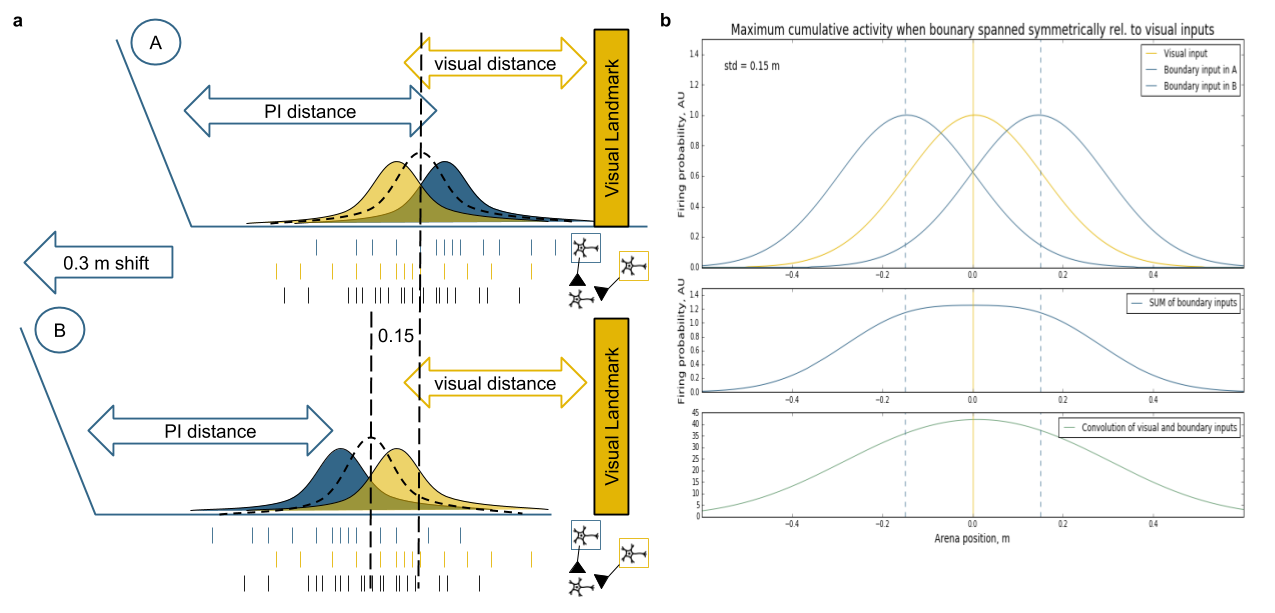
\includegraphics[width=150mm]{figures/F39_symmetric_encoding.png}}
\caption[Symmetric encoding]{
Symmetric positioning of self-motion inputs around visual input can lead to an average encoding. (a) When position relative to both reference frames is always in conflict, the higher probability of mutual spiking will happen to sensory afferents shifted 0.15m relative to each other in both conditions. (b) In cases of small conflicts the convolution of the putative visual and self-motion place afferents is highest when they are shifted 0.15m relative to each other like in (a).
}
\label{fig:F39_symmetric_encoding}
\end{figure}

Assuming all inputs do have regular gaussian spiking probability, this could be confirmed by computing the convolution between the stable visual input and both self-motion driven inputs in both conditions, located 0.3m apart from each other. If place field sizes relative to the longitudinal arena shift are large enough, the maximum convolution will be when the visual input is located symmetrically between self-motion inputs (in our case an average field size of 0.4m, Figure 39b) Even if the two original and shifted conditions never appear at the same time, some potential accumulation of the total mutual spiking of these visual and symmetrically located self-motion inputs and a postsynaptic neuron can lead to an increased connection by hebbian plasticity, resulting in this half-distance situation.


\subsection{Behavior of multisensory cells can be explained by dynamic loops in the hippocampal-entorhinal network}

However, the actual mechanisms could be more complicated. A recent modelling work of a entorhinal-hippocampal system, assuming necessary involvement of recurrent connections from the CA1 to the EC region (\cite{Li2020}), can explain the half-distance shift phenomena. The dynamic loop-based network model, tested against the multi-compartment experimental data (\cite{Carpenter2015}; \cite{Wernle2018}), demonstrates the same effect on the level of CA1 place cells when self-motion and visual cues are in conflict. Authors performed a simulation of the condition with gain between the vision and self-motion in a similar rectangular arena-like experiment, and found that the population of place cells shifts to the intermediate position between the self-motion and visual estimates. This effect is explained by the dynamic loop-like interaction between the visually-driven place cells and populations of grid cells, which are shifted by them towards the visually identified location. To verify this hypothesis a more precisely defined gain experiment can be designed and implemented.


\section{Aspects of using freely-moving virtual reality system}
\label{sec:aspects_of_vr}

The use of the freely-moving virtual reality system has its advantages but also potential drawbacks. As all conventional virtual reality systems, ratCAVE is an excellent instrument for visual manipulations and induction of a visual to movement mismatch, in a closed-loop with the computation of the animal position. The freely-moving condition is far more naturalistic compared to the head or body fixed conditions, where certain internal (vestibular, proprioceptive) and external (feeling of boundaries) information is not present. It also allows for easier and shorter training protocols (\cite{Ferreiro2020}) avoiding any animal fear states.

The existence of boundaries might be of a special importance as the boundary driven cells have significant impact on the place code (\cite{Okeefe1996}; \cite{Barry2006}; \cite{Savelli2008}). Environmental boundaries play a special role in the formation of a spatial map, without physical contact with the walls, as it is usually in conventional virtual reality systems, the map of space at the level of place cells might not be complete.

However, the same issue can be applied to the ratCAVE. The 3D virtual reality setup allows placing 3D virtual objects inside the arena, not just having visual proximal or unreachable distal landmarks on the walls. Although this makes the virtual environment more immersive, absence of the physical tactile contact with virtual objects might affect their representation in the brain, potentially reducing their significance for the spatial map. In particular, object vector cells (\cite{Hooydal2019}), which play an important role in spatial coding, might be affected. Favourably, current experimental results demonstrate strong influence of the visual cues on the hippocampal place cells, so the overall influence of visual virtual objects is doubtless - however the amount of the mismatch between visual object appearance and their tactile insensitivity is to be identified.


\section{Aspects of experimental design}
\label{sec:aspects_of_design}

I recorded several sessions of the shift and gain experiments with the same cohort of animals. Theoretically, this might bias the experimental data in a few ways.

First, after several sessions being in the same experimental protocol, animals can better learn the environment and understand that the projected visual reference frame is not required to get food rewards. This might influence the amount of visual place encoding down to complete ignorance of the virtual reference frame. To account for that, tests for the difference in the amount of visually or self-motion selective cells across days were done. They do not show any difference.

Second, some animals were used in both shift and gain experiment types. Hypothetically, the knowledge of one virtual environment may influence the behavior of cells in another condition - as both virtual shift and gain environments are the same, the knowledge of the environment in one condition (e.g. shift) might cause activation of the same cells in another condition (e.g. gain), which would not happen otherwise due to, for instance, ignorance of the visual flow because of the proprioceptive mismatch. To be sure to exclude this influence, experiments with separated cohorts of animals should be performed.


\section{Open questions}
\label{sec:open_questions}

It is still not clear at which stage the integration of the self-motion and external sensory information is done. One possibility for the multisensory neurons would be to integrate recurrent inputs from the same CA1 - CA3 circuit, basically working with the same visually- and boundary-defined cells in CA1. Another possibility would be to get direct self-motion and sensory inputs from the mEC / lEC. An opportunity to test these options would be to perturb entorhinal inputs to the hippocampus while recording the shift experiment and investigate the change of activity of the multisensory neurons.

Apart from that, data showing the integration of the inputs on the hippocampal level confirms the idea of a hippocampus as a general memory device - providing mechanisms to match and update neuronal firing patterns representing recurrently occuring episodes, that allows to implement stable place fields, like any memory sharpens and stabilizes with repeats. Further design of experimental protocols with gradual visual virtual cue manipulations could provide more insights into the mechanisms of pattern completion and pattern separation - investigating the stability of the recorded place fields, or a change in the place field firing depending on the changes in the virtual environment.


\chapter{Conclusion and outlook}

This master's thesis was originally motivated by the desire to automatically interpret data sets and generate hypotheses using prior knowledge. While working towards that goal, it was necessary to develop an entire computational infrastructure for BEL. That infrastructure was extended with reusable components to integrate prior knowledge from other sources in order to model biology at the finest granularity possible. Next, a framework for testing the validity and robustness of those knowledge assemblies was implemented and applied to the \ac{NeuroMMSig} knowledge base. Finally, algorithms for extracting meaningful subnetworks were applied to enable schema-free and multi-modal analysis using a heat diffusion algorithm. Using this workflow, it is now possible to interpret multi-modal data sets and generate hypotheses in a truly automated fashion.


\printbibliography

\backmatter

\chapter{List of publications}

\underline{First author:}

\textbf{Sobolev, A.}, Stoewer, A., Leonhardt, A., Rautenberg, P. L., Kellner, C. J., Garbers, C., \& Wachtler, T. (2014). Integrated platform and API for electrophysiological data. Frontiers in Neuroinformatics, 8(APR).
https://doi.org/10.3389/fninf.2014.00032

\textbf{Sobolev, A.}, Stoewer, A., Leonhardt, A., Rautenberg, P. L., Kellner, C. J., Garbers, C., \& Wachtler, T. (2014). Integrated platform and API for electrophysiological data. Frontiers in Neuroinformatics, 8(APR).
https://doi.org/10.3389/fninf.2014.00032

\underline{co-author:}

Ferreiro, D. N., Amaro, D., Schmidtke, D., \textbf{Sobolev, A.}, Gundi, P., Belliveau, L., Sirota, A., Grothe, B., \& Pecka, M. (2020). Sensory Island Task (SIT): A New Behavioral Paradigm to Study Sensory Perception and Neural Processing in Freely Moving Animals. Frontiers in Behavioral Neuroscience, 14.
https://doi.org/10.3389/fnbeh.2020.576154

Zehl, L., Jaillet, F., Stoewer, A., Grewe, J., \textbf{Sobolev, A.}, Wachtler, T., Brochier, T. G., Riehle, A., Denker, M., \& Grün, S. (2016). Handling metadata in a neurophysiology laboratory. Frontiers in Neuroinformatics, 10(JUL).
https://doi.org/10.3389/fninf.2016.00026

Garcia, S., Guarino, D., Jaillet, F., Jennings, T., Pröpper, R., Rautenberg, P. L., Rodgers, C. C., \textbf{Sobolev, A.}, Wachtler, T., Yger, P., \& Davison, A. P. (2014). Neo: An object model for handling electrophysiology data in multiple formats. Frontiers in Neuroinformatics, 8(FEB).
https://doi.org/10.3389/fninf.2014.00010

Rautenberg, P. L., \textbf{Sobolev, A.}, Herz, A. V. M., \& Wachtler, T. (2011). A database system for electrophysiological data. In Lecture Notes in Computer Science (including subseries Lecture Notes in Artificial Intelligence and Lecture Notes in Bioinformatics): Vol. 6990 LNCS.
https://doi.org/10.1007/978-3-642-23740-9



\chapter{Affidavit}
Hiermit versichere ich an Eides statt, dass ich die vorliegende Dissertation selbstständig angefertigt habe, mich außer der angegebenen keiner weiteren Hilfsmittel bedient und alle Erkenntnisse, die aus dem Schrifttum ganz oder annähernd übernommen sind, als solche kenntlich gemacht und nach ihrer Herkunft unter Bezeichnung der Fundstelle einzeln nachgewiesen habe.

I hereby confirm that this dissertation is the result of my own work and that I have only used sources or materials listed and specified in the dissertation.


\vspace{0.3in}

\noindent Munich, \today

\vspace{1in}

\noindent Andrey Sobolev


\chapter{Author Contributions}
Andrey Sobolev, Dr. Kay Thurley, Dr. Dustin Fetterhoff, Prof. Dr. Christian Leibold and Prof. Dr. Anton Sirota contributed to this research study.

The project was established by Anton Sirota, Christian Leibold and Kay Thurley. The design of the experimental protocols and the virtual environment was done by Andrey Sobolev with the support of Anton Sirota. Animal handling was performed by Andrey Sobolev under the guidance of Kay Thurley. Printing and assembling implants as well as the surgical procedures were done by Andrey Sobolev. Dustin Fetterhoff contributed with animals from his project to the study. Data analysis was done by Andrey Sobolev under review of Anton Sirota and Christian Leibold.

We assert that aforementioned author contributions are correct and accurate:

\vspace{0.3in}

\noindent Munich, \today

\vspace{0.5in}

\noindent Andrey Sobolev

\vspace{0.5in}

\noindent Prof. Dr. Anton Sirota


\end{document}
